\documentclass{mini}
\usepackage[utf8]{inputenc}
\usepackage{fancyvrb}
\usepackage{amsmath}
\usepackage{subfig}
\newcommand{\degree}{\ensuremath{^\circ}}
\newcommand{\hilight}[1]{\colorbox{yellow}{#1}}
\linespread{1.5}
\newcommand{\CMAES}{\mbox{CMA-ES}}
\DeclareUnicodeCharacter{00A0}{~}

%------------------------------------------------------------------------------%
\title{Analiza możliwości wykorzystania w~algorytmie CMA-ES wiedzy o~ograniczeniach kostkowych}

\author{inż. Robert Jakubowski}
\supervisor{dr hab. inż. Jarosław Arabas prof. nzw. PW}
\type{magisters}
\monthyear{Maj 2016}
\date{\today}
\album{237545}
%------------------------------------------------------------------------------%
\begin{document}

\maketitle

\pagebreak
\thispagestyle{empty}

\openup -0.2em %make it fit on one page
\tableofcontents
\openup 0.2em %make it fit on one page

\thispagestyle{empty}
\raggedbottom
\pagebreak


\section{Streszczenie}

Praca bada wpływ różnych metod uwzględniania ograniczeń w algorytmie CMA-ES. Wyniki badań przeanalizowane są w celu sprawdzenia, czy można wykorzystać informacje o ograniczeniach kostkowych w tymże algorytmie.

We wstępie został przedstawiony przedmiot badań oraz cel pracy - sprawdzenie możliwości poprawy algorytmu CMA-ES.

Po wstępie opisano algorytm CMA-ES. Teoretyczna analiza tego algorytmu jest niezbędna do zrozumienie jego mechanizmów, a w konsekwencji do przeprowadzenia badań. Z tego samego względu opisano również techniki uwzględniania ograniczeń. W rozdziale poświęconym ograniczeniom zawarto nie tylko opisy poszczególnych metod, ale również pokazano w sposób empiryczny jak mogą wpływać na algorytmy. W tym celu użyto algorytmu błądzenia przypadkowego. Zaimplementowano ten algorytm z różnymi wariantami uwzględniania ograniczeń, a następnie przeprowadzono szereg testów badających między innymi rozkłady prawdopodobieństw oraz wartości oczekiwanych.

Następny rozdział opisuje sposoby, w jaki mogą być testowane algorytmy optymalizacji globalnej. Niezbędne do testowania są specjalnie przygorowane funkcje benchmarkowe, które badają skuteczność algorytmów. W tej części przedstawiono również test Wilcoxona, który wykorzystuje się do porównania wyników funkcji benchmarkowych.

Opisane metody testowania zostały użyte w  rozdziale, który przedstawia testy wykonane na algorytmie CMA-ES oraz jego modyfikacjach. Modyfikacje polegały wyłącznie na zmiane metod uwzględniania ograniczeń. Wyniki zostały zebrane i ze sobą porównane.

W ostatnim rozdziale zebrane są obserwacje poczynione w pracy. Rozdzaił ten, to również wskazanie możliwości poprawy algorytmu CMA-ES.

\pagebreak

\section{Wstęp}
Algorytmy ewolucyjne wykorzystuje się głównie w problemach z wieloma zmiennymi, np. w planowaniu procesów przemysłowych.\cite{zast} Klasyczne algorytmy ewolucyjne nie dostosowują się do charakterystyki optymalizowanej funkcji. W~większości z nich rozkład prawdopodobieństwa generowanych punktów nie zmienia się w trakcie symulacji algorytmu. Z~tego faktu wynika problem ustalenia parametrów początkowych, np. wariancji rozkładu prawdopodobieństwa. Ustalenie zbyt niskiej wartości wariancji może prowadzić do znalezienia jedynie pewnego optimum lokalnego, natomiast ustalenie zbyt dużej wartości wariancji sprawia, że trudno znaleźć algorytmowi optimum globalne.

Na przeciw problemowi ustalenia wariancji wychodzi algorytm CMA-ES. Już samo rozwinięcie akronimu CME-ES mówi o tym: Covariance Matrix Adaptation - Evolution Strategy (adaptacja macierzy kowariancji -~strategia ewolucyjna). Jest to algorytm oparty na technikach ewolucyjnych, aczkolwiek punkty losowane są na podstawie macierzy kowariancji (wielowymiarowe uogólnienie wariancji), która jest w każdej iteracji dostosowywana do aktualnej sytuacji przeszukiwań. Takie rozwiązanie sprawia, że dobór parametrów początkowych nie jest tak istotny jak w innych algorytmach ewolucyjnych.

CMA-ES jest algorytmem dość skomplikowanym w szczegółach - można się o tym przekonać czytając rozdział \ref{secalgcmaes}, który jest poświęcony teoretycznemu opisowi tegoż algorytmu. Mimo kilkunastu lat istnienia podejmowane są kolejne próby jego optymalizacji (\cite{magist}\cite{lcmaes}). Warto jednocześnie pamiętać, że w większości wariantów algorytmu CMA-ES trudno mówić o uniwersalnej optymalizacji. Zazwyczaj poprawa w pewnej grupie funkcji skutkuje pogorszeniem wyników w innym rodzaju funkcji.

Ta praca jest próbą optymalizacji algorytmu CMA-ES skoncentrowaną na ograniczeniach kostkowych. Ograniczenia napotykamy w wielu problemach - materiały mają wytrzymałość, komputery skończoną pamięć, a czasem ogranicza prędkość światła.

W aktualnej wersji algorytmu CMA-ES punkty, które znajdą się poza ograniczeniem, są na to ograniczenie rzutowane (o rzutowaniu można przeczytać w rozdziale \ref{secrzut}). Jest to tylko jedna z metod uwzględniania ograniczeń. Warto zauważyć, że zamiast rzutować punkt na ograniczenie, można go reinicjować, powtórnie losować, czy też przekształcić symetrycznie względem ograniczeń.

\subsection*{Cel pracy}
Celem pracy jest sprawdzenie, w jaki sposób można poprawić algorytm CMA-ES. Analiza będzie skupiała się na ograniczeniach kostkowych. Cel będzie realizowany poprzez teoretyczne roważania oraz przeprowadzenie testów.

\pagebreak

\section{Algorytm CMA-ES} \label{secalgcmaes}

Zgodnie z tym, co zostało ustalone we wstępie, algorytm CMA-ES należy do rodziny algorytmów ewolucyjnych. Cechą wyróżniającą ten algorytm jest specyficzny sposób generowania punktów. Można to zauważyć w poniższym pseudokodzie opisującym algorytm CMA-ES (równania są cytowaniami z \cite{cmaes_tutorial}):
\begin{Verbatim}
inicjalizuj zmienne
dopóki nie są spełnione warunki stopu:
	generuj punkty
\end{Verbatim}
\hspace{12ex} $x_k^{t+1} \sim m^t + \sigma^tN(0,C^t)$
\begin{Verbatim}
	oblicz wartości funkcji w wygenerowanych punktach
	posortuj punkty
\end{Verbatim}
\hspace{12ex} $f(x_{1:\lambda}^{t+1}) \leq f(x_{2:\lambda}^{t+1}) \leq ... \leq f(x_{\lambda:\lambda}^{t+1})$
\begin{Verbatim}
	przeprowadź selekcję punktów
	oblicz wartość oczekiwaną rozkładu
\end{Verbatim}
\hspace{12ex} $m^{t+1}=m^t+c_m\sum\limits_{i=1}^\mu w_i(x_{i:\lambda}^{t+1}-m^t)$
\begin{Verbatim}
	oblicz długość kroku
\end{Verbatim}
\hspace{12ex} $p_\sigma^{t+1}=(1-c_\sigma)p_\sigma^t+\sqrt{c_\sigma(2-c_\sigma)\mu_{eff}}{C^t}^{-\frac{1}{2}}\frac{m^{t+1}-m^t}{\sigma^t}$

\hspace{8,5ex} $\sigma^{t+1}=\sigma^t exp (\frac{c_\sigma}{d_\sigma}(\frac{\|p_\sigma^{t+1}\|}{E\|N(0,I)\|}-1))$
\begin{Verbatim}
	oblicz macierz kowariancji
\end{Verbatim}
\hspace{12ex} $p_c^{t+1} = (1-c_c)p_c^t+\sqrt{c_c(2-c_c)\mu_{eff}}\frac{m^{t+1}-m^t}{\sigma^t}$

\hspace{8,5ex} $C^{t+1} = (1-c_1-c_\mu\sum\limits_{j=1}^\lambda w_j)C^t+c_1p_c^{t+1}{(p_c^{t+1})}^T+c_\mu \sum\limits_{i=1}^\lambda w_iy_{i:\lambda}^{t+1}{(y_{i:\lambda}^{t+1})}^T$
\newline
gdzie:
\begin{itemize}[noitemsep]
\item $x_k^t$ - k-ty punkt iteracji numer t
\item $m^t$ - wartość oczekiwana rozkładu w iteracji t
\item $\sigma^t$ - długość kroku iteracji t
\item $N(p,C)$ - losowanie punktu z rozkładem normalnym o wartości oczekiwanej w punkcie p oraz macierzy kowariancji C
\item $C^t$ - macierz kowariancji iteracji t
\item $f(x)$ - wartość funkcji w punkcie x
\item $\lambda$ - wielkość populacji (ilość punktów x w jednej iteracji)
\item $c_m$ - współczynnik nauki wartości oczekiwanej
\item $\mu$ - liczba wybieranych punktów spośród wszystkich $\lambda$ punktów (patrz \ref{selekcjapunktow} Selekcja punktów)
\item $w_i$ - waga punktu $x_i$
\item $p_\sigma^t$ - sprzężona ścieżka ewolucji w iteracji t
\item $c_\sigma$ - współczynnik nauki długości kroku
\item $\mu_{eff}=\frac{1}{\sum\limits_{i=1}^\mu w_i^2}$
\item $d_\sigma \approx 1$ - stała tłumienia
\item $p_c^t$ - ścieżka ewolucji w iteracji t
\item $c_c$ - współczynnik nauki macierzy kowariancji
\item $c_1 \approx \frac{2}{n^2}$ 
\item $c_\mu \approx min(\frac{\mu_{eff}}{n^2}, 1-c_1)$
\item $y_{i:\lambda}^{t+1} = \frac{x_{i:\lambda}^{t+1}-m^t}{\sigma^t}$
\end{itemize}

Cały algorytm jest dość skomplikowany. Najważniejsze części są opisane poniżej w następującej kolejności: macierz kowariancji, wartość oczkiwana rozkładu, długość kroku, generowanie punktów, selekcja punktów.

\subsection{Macierz kowariancji} \label{macierz}
Punkty w algorytmie CMA-ES są generowanie poprzez losowanie na podstawie macierzy kowariancji. Oznacza to, że nie istnieje bezpośredni związek pomiędzy punktami kolejnych iteracji - w~klasycznych algorytmach ewolucyjnych zazwyczaj można było mówić o rodzicach wygenerowanego punktu. Punkty wpływają jednak na macierz kowariancji, a pośrednio przez nią na kolejną generację punktów. Odbywa się to w następujący sposób: z populacji punktów wybiera się $\mu$ punktów (zazwyczaj połowę), która zwraca lepsze wartości funkcji celu. Następnie przypisuje się im wagi - w zależności od tego, jak dobry jest punkt. Na postawie tych danych wyznaczana jest empiryczna macierz kowariancji.

\subsection{Wartość oczekiwana rozkładu} \label{wartoscoczekiwana}
Punkty generowane są na podstawie rozkładu określonego macierzą kowariancji. Sama macierz nie mówi jednak nic o wartości oczekiwanej. Wymaga to oddzielnego wyznaczenia tej wartości.

Podobnie jak w przypadku macierzy kowariancji, wybiera się $\mu$ punktów. Dla tych punktów wyznaczane są wektory przesunięć względem wartości oczekiwanej (każdy wektor jest skalowany przez wagę punktu). Wektory te sumujemy otrzymując pewien wektor wynikowy, który następnie jeszcze skalujemy przez współczynnik nauki. O tak otrzymany wektor przesuwamy dotychczasową wartość oczekiwaną.

\subsection{Długość kroku}
Generowanie punktów z macierzy kowariancji pozwala na skalowanie tego rozkładu poprzez dodanie jednego parametru. Ten parametr jest nazywany długością kroku. W~algorytmie CMA-ES długość kroku obliczana jest na podstawie kierunku przemieszczania się wartości oczekiwanej rozkładu. Długość kroku zwiększa się, gdy wartość oczekiwana przemieszcza się w tym samym kierunku. Skraca natomiast, gdy kierunek jest zmienny.

\subsection{Generowanie punktów}
Punkty są generowane poprzez wylosowanie wektora liczb na postawie macierzy kowariancji. Wylosowany wektor jest skalowany przez długość kroku, a na koniec jest przesuwany o wektor równy wartości oczekiwanej rozkładu.

\subsection{Selekcja punktów} \label{selekcjapunktow}
Selekcja punktów, to wybór $\mu$ punktów spośród całej populacji. Wybierane są te punkty, które mają lepszą wartość funkcji. Wartość funkcji wpływa również na przypisywane punktom wagi, o których wspomniano wcześniej.

\pagebreak

\section{Techniki uwzględniania ograniczeń}
Niektóre problemy optymalizacyjne posiadają ograniczenia. Szukając rozwiązania należy zapewnić, że będzie ono dopuszczalne. Bazując na \cite{wyklady} techniki uwzględniania ograniczeń można podzielić ze względu na wykorzystanie:
\begin{itemize}[noitemsep]
\item definicji przestrzeni przeszukiwań - zapewnienie, że podczas krzyżowań, mutacji i innych zmian punktów, żaden z punktów nie wypadnie poza przestrzeń przeszukiwań,
\item modyfikacji funkcji celu - zmienienie funkcji celu tak, aby funkcja celu dla punktów spoza ograniczeń zwracały gorsze wyniki,
\item transformacji rozwiązań - punkty, które są poza ograniczeniami zostają zamieniane na punkty, które znajdują się w ograniczeniach.
\end{itemize}

Każda z tych technik posiada wiele wariantów. Przeanalizowanie wszystkich mogłoby być bardzo czasochłonne. W związku z tym w tej pracy skupiono się na transformacji rozwiązań.

\subsection{Transformacje rozwiązań} \label{transformacje}
Istnieje wiele technik transformacji rozwiązań. W~kolejnych podrozdziałach znajdują się metody transformacji, które były badane na potrzeby tej pracy. Każda z technik jest opisana słownie oraz pseudokodem. Opis słowny zawiera wyjaśnienie, co się dzieje z punktem, który znalazł się poza ograniczeniem. W~pseudokodzie zastosowano następujące oznaczenia:
\begin{itemize}[noitemsep]
\item $x$ - punkt, który poddajemy naprawie
\item $x'$ - rodzic punktu $x$; z punktu $x'$ z zadanym rozkładem został wygenerowany punkt $x$
\item $x(i)$ - wartość $i$-tej współrzędnej punktu $x$
\item $lb$ - ograniczenie dolne
\item $ub$ - ograniczenie górne
\end{itemize}

\subsubsection{Metoda klasyczna}
Nowy punkt zostaje odrzucony i wraca do poprzedniej pozycji.

\begin{Verbatim}[baselinestretch=1.1]
	x = x'
\end{Verbatim}


\subsubsection{Rzutowanie}
\label{secrzut}
Punkt jest transformowany do najbliższego punktu, który spełnia ograniczenia. Oznacza to, że dla każdej współrzędnej sprawdzany jest warunek zawierania się w ograniczeniach. Wartości współrzędnych, dla których nie jest on spełniony, zmieniane są na wartości ograniczeń (odpowiednio dolne lub górne), które są najbliżej.

\begin{Verbatim}[baselinestretch=1.1]
	dla każdej współrzędnej i
		jeżeli lb(i) > x(i)
			x(i) = lb(i)
		jeżeli ub(i) < x(i)
			x(i) = ub(i)
\end{Verbatim}

\subsubsection{Reinicjacja} \label{reinicjacja}
Punkt jest przenoszony do pozycji początkowej.

\begin{Verbatim}[baselinestretch=1.1]
	x = x0
\end{Verbatim}

\subsubsection{Próbkowanie}
Punkt jest powtórnie generowany do momentu, aż spełni ograniczenie kostkowe.

\begin{Verbatim}[baselinestretch=1.1]
	dopóki !w_ograniczeniach(x)
		x = losuj(x')
\end{Verbatim}

\subsubsection{Zawijanie}
Dla każdej współrzędnej sprawdzane są warunki ograniczeń. W przypadku współrzędnych, na których punkt jest poza ograniczeniem, różnica pomiędzy ograniczeniem a wartością współrzędnej punktu jest zapamiętywana. Tę różnicę odkładamy na przeciwległym ograniczeniu po stronie, która jest wewnątrz ograniczeń. W tym miejscu znajduje się nowa wartość współrzędnej punktu. Z perspektywy punktu nie ma ograniczeń, a przestrzeń przeszukiwań po każdym wymiarze jest jakby "zawinięta".

\begin{Verbatim}[baselinestretch=1.1]
	dla każdej współrzędnej i
		jeżeli lb(i) > x(i)
			x(i) = ub(i) - (lb(i) - x(i))
		jeżeli ub(i) < x(i)
			x(i) = lb(i) + (x(i) - ub(i))
\end{Verbatim}

\subsubsection{Odbicie}
Dla każdej współrzędnej sprawdzane są warunki ograniczeń. W przypadku współrzędnych, na których punkt jest poza ograniczeniem, wartość punktu tej współrzędnej jest symetrycznie odbita względem ograniczenia, którego warunek został złamany.

\begin{Verbatim}[baselinestretch=1.1]
	dla każdej współrzędnej i
		jeżeli lb(i) > x(i)
			x(i) = x(i) + 2 * (lb(i) - x(i))
		jeżeli ub(i) < x(i)
			x(i) = x(i) - 2 * (x(i) - ub(i))
\end{Verbatim}

\subsection{Błądzenie przypadkowe} \label{bladzenie}

Można się spodziewać, że algorytm CMA-ES dla funkcji stałej będzie zachowywał się analogicznie do błądzenia przypadkowego. Takie założenie skłoniło autora, żeby zbadać błądzenie przypadkowe z ograniczeniami. Błądzenie przypadkowe jest algorytmem prostszym niż CMA-ES, więc umożliwia szybsze testowanie i wyciąganie wniosków.

Niech $ X_1, X_2, ... $ będą niezależnymi n-wymiarowymi zmiennymi losowymi o wartości oczekiwanej równej $ [0]^n $. Błądzeniem przypadkowym nazywamy sekwencję punktów $S_1$, $S_2$, ..., takich że:

\begin{equation}
S_1 = X_1, S_i=S_{i-1}+X_i
\end{equation}

Zmienne losowe mogą być realizowane w różny sposób. Mogą to być wektory o~rozkładzie normalnym, jednostajnym lub innym.

\subsection{Metoda przeprowadzania testów}
Celem testów jest zaobserwowanie, jaki wpływ na symulację ma metoda uwzględniania ograniczeń. Do tak postawionego celu można podejśc na różne sposby. Wybrano 2 cechy, które miały zrealizować postawiony cel:
\begin{enumerate}
\item Wartość oczekiwana generowanego punktu (razem z poprawą).
\item Rozkład prawdopodobieństwa generowanych punktów.
\end{enumerate}

Sposoby testowania obu cech są opisane w kolejnych podrozdziałach.

\subsubsection{Wartość oczekiwana generowanego punktu}
Wartością oczekiwaną liczby $X_i$ w błądzeniu przypadkowym jest 0. Implikuje to fakt, że wartością oczekiwaną $S_i$ jest $S_{i-1}$. Ustalenie ograniczeń kostkowych powoduje, że nadal losujemy liczbę $X_i$, której wartość oczekiwana jest równa 0. Dodajemy jednak metody naprawy. W związku z tym wartością oczekiwaną $S_i$ nie zawsze jest $S_{i-1}$.

Dla każdego punktu $p$ przestrzeni przeszukiwań można przypisać wektor $\overrightarrow{d}$. Początek $\overrightarrow{d}$ znajduje się w $p$. Załóżmy teraz, że $p$ jest punktem $S_i$ pewnego błądzenia przypadkowego z ograniczeniami. Koniec wektora $\overrightarrow{d}$ znajduje się w wartości oczekiwanej punktu $S_{i+1}$.

Wykres, który będzie zawierał wektory $\overrightarrow{d}$, pozwoli na określenie charakterystyki przemieszczania się punktów w poszczególnych częściach przestrzeni przeszukiwań.

\subsubsection*{Implementacja}
Do wizualizacji wybrano symulację, w której punkty posiadają 2 wymiary. Pozwala to na przejrzystą wizualizację wektorów dla każdego z punktów. Pokazuje też zachowanie wektorów w rogach - punktach, które są blisko kilku ograniczeń.

Dla każdego z 2 wymiarów wybrano kilkanaście, równoodległych punktów. W skład tych punktów wchodziły też punkty znajdujące się na ograniczeniach. Następnie stworzono 2 pętle po tych punktach (jedna zagnieżdżona w drugiej). W ten sposób uzyskano regularnie rozłożone punkty w dwóch wymiarach.

Dla każdego z tych punktów przeprowadzono następujące obliczenia. 1000 razy uruchomiono symulację jednego kroku algorytmu błądzenia przypadkowego (z rozkładem normalnym) z odpowiednią naprawą. Otrzymano tysiąc punktów, z których następnie obliczono średnią arytmetyczną. Tak uzyskany punkt potraktowano jako wartość oczekiwaną i wyrysowano wektor $\overrightarrow{d}$.

\subsubsection{Rozkład prawdopodobieństwa generowanych punktów}
Punkty w błądzeniu przypadkowym poruszają się chaotycznie. Ta losowość jest częściowo uporządkowana na ograniczeniach. W zależności od metody naprawy, punkty zachowują się inaczej, a rozkład prawdopodobieństwa jest zniekształcony. Autor postanowił przyjrzeć się jak wygląda rozkład prawdopodobieństwa wystąpienia punktu z~perspektywy całej symulacji.

Dla każdej metody naprawy opisanej w \ref{transformacje} jednokrotnie uruchomiono algorytm błądzenia przypadkowego jednego punktu. Oddzielnie symulowano również błądzenie z rozkładem normalnym oraz jednostajnym na przedziale $[-0.5; 0.5]$ (przedział co najmniej kilkukrotnie krótszy od ograniczeń kostkowych). Po każdej iteracji nowo wygenerowany punkt zapisywano w tablicy. Z tak przygotowanej tablicy generowano histogram.

\subsubsection*{Implementacja}
Dla każdej z metod naprawy przygotowano oddzielny skrypt. Pseudokod skryptu zamieszczono poniżej.
\begin{Verbatim}[baselinestretch=1.1]
	x - błądzący punkt
	punkty - tablica wszystkich położeń punktu x
	iteracje - liczba iteracji podana jako parametr
	i = 0
	dopóki i < iteracje
		d = wektor wylosowany z zadanym rozkładem
		x = x + d
		jeżeli x jest poza ograniczeniem
			popraw x
		dodaj x do tablicy punkty
		i = i + 1
\end{Verbatim}

\subsection{Wyniki testów}
Wykresy zamieszczone w tym podrozdziale są 2 rodzajów. Są to wykresy wektorów $\overrightarrow{d}$ wartości oczekiwanych oraz histogramamy wystąpień punktu.

Histogramy były tworzone poprzez symulację skryptów z liczbą iteracji wynoszącą \mbox{2-100} milionów. Szerokość przedziałów jest różna i była dobierana tak, aby jak najlepiej przedstawić interesujące fakty. Wszystkie wykresy, które pokazdują wyniki błądzenia przypadkowego w dwóch wymiarach zostały przetworzone w następujący sposób: otrzymane wyniki symulacji powielono poprzez symetrzyczne odbicie ich względem osi X, osi Y oraz początku układu współrzędnych. Wykonano ten zabieg, aby zwiększyć dokładność wyników. Nie wpływają one na badania, ponieważ punkty 0 są środkami ograniczeń obu osi, a z perspektywy algorytmu nie ma znaczenia, w której ćwiartce znajduje się aktualnie punkt.

\subsubsection*{Metoda klasyczna}
Wektory wartości oczewkianych, które są blisko ograniczeń są skierowane od ograniczenia. Histogramy z kolei pokazują, że punkty z większym prawdopodobieństwem występują przy ograniczeniach. Takie zachowanie wynika z tego, że potomkowie punktów blisko granicy mogą "wypaść" poza ograniczenie. Po naprawie dziecko będzie tym samym punktem.

\begin{figure}[H]
\centering
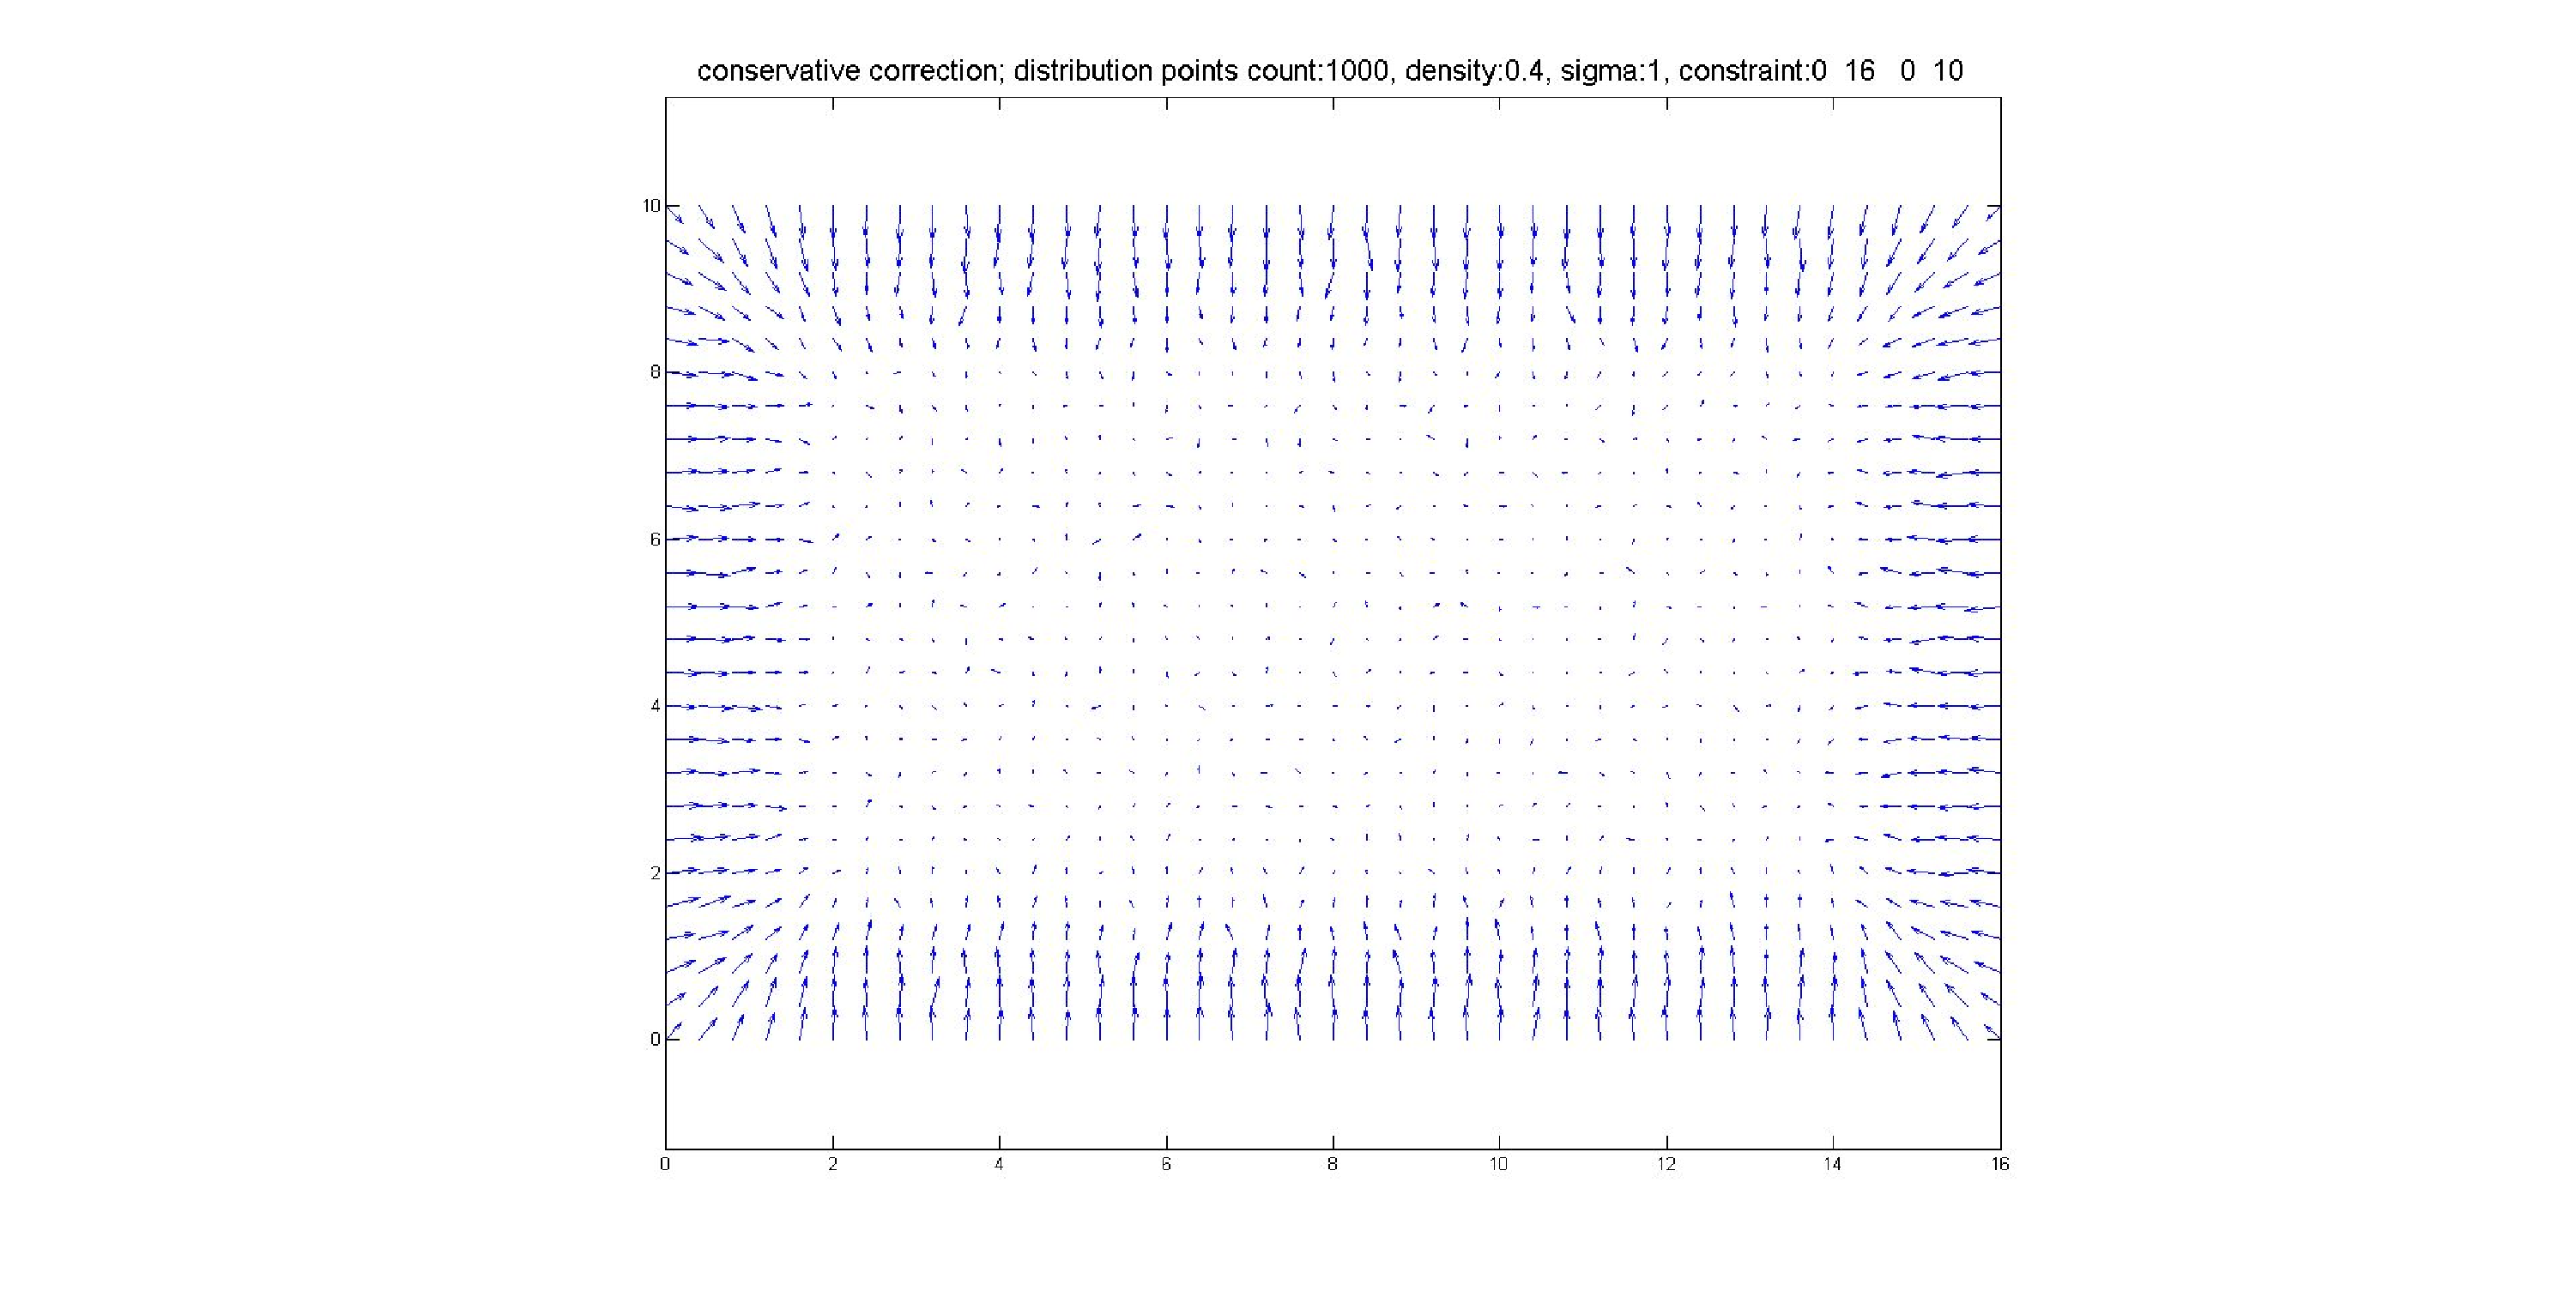
\includegraphics[width=\textwidth]{conservative2dprzesuniecie}
\caption{Wartość oczekiwana punktu}
\end{figure}

\begin{figure}[H]
\centering
\subfloat[Generowanie z rozkładem normalnym]{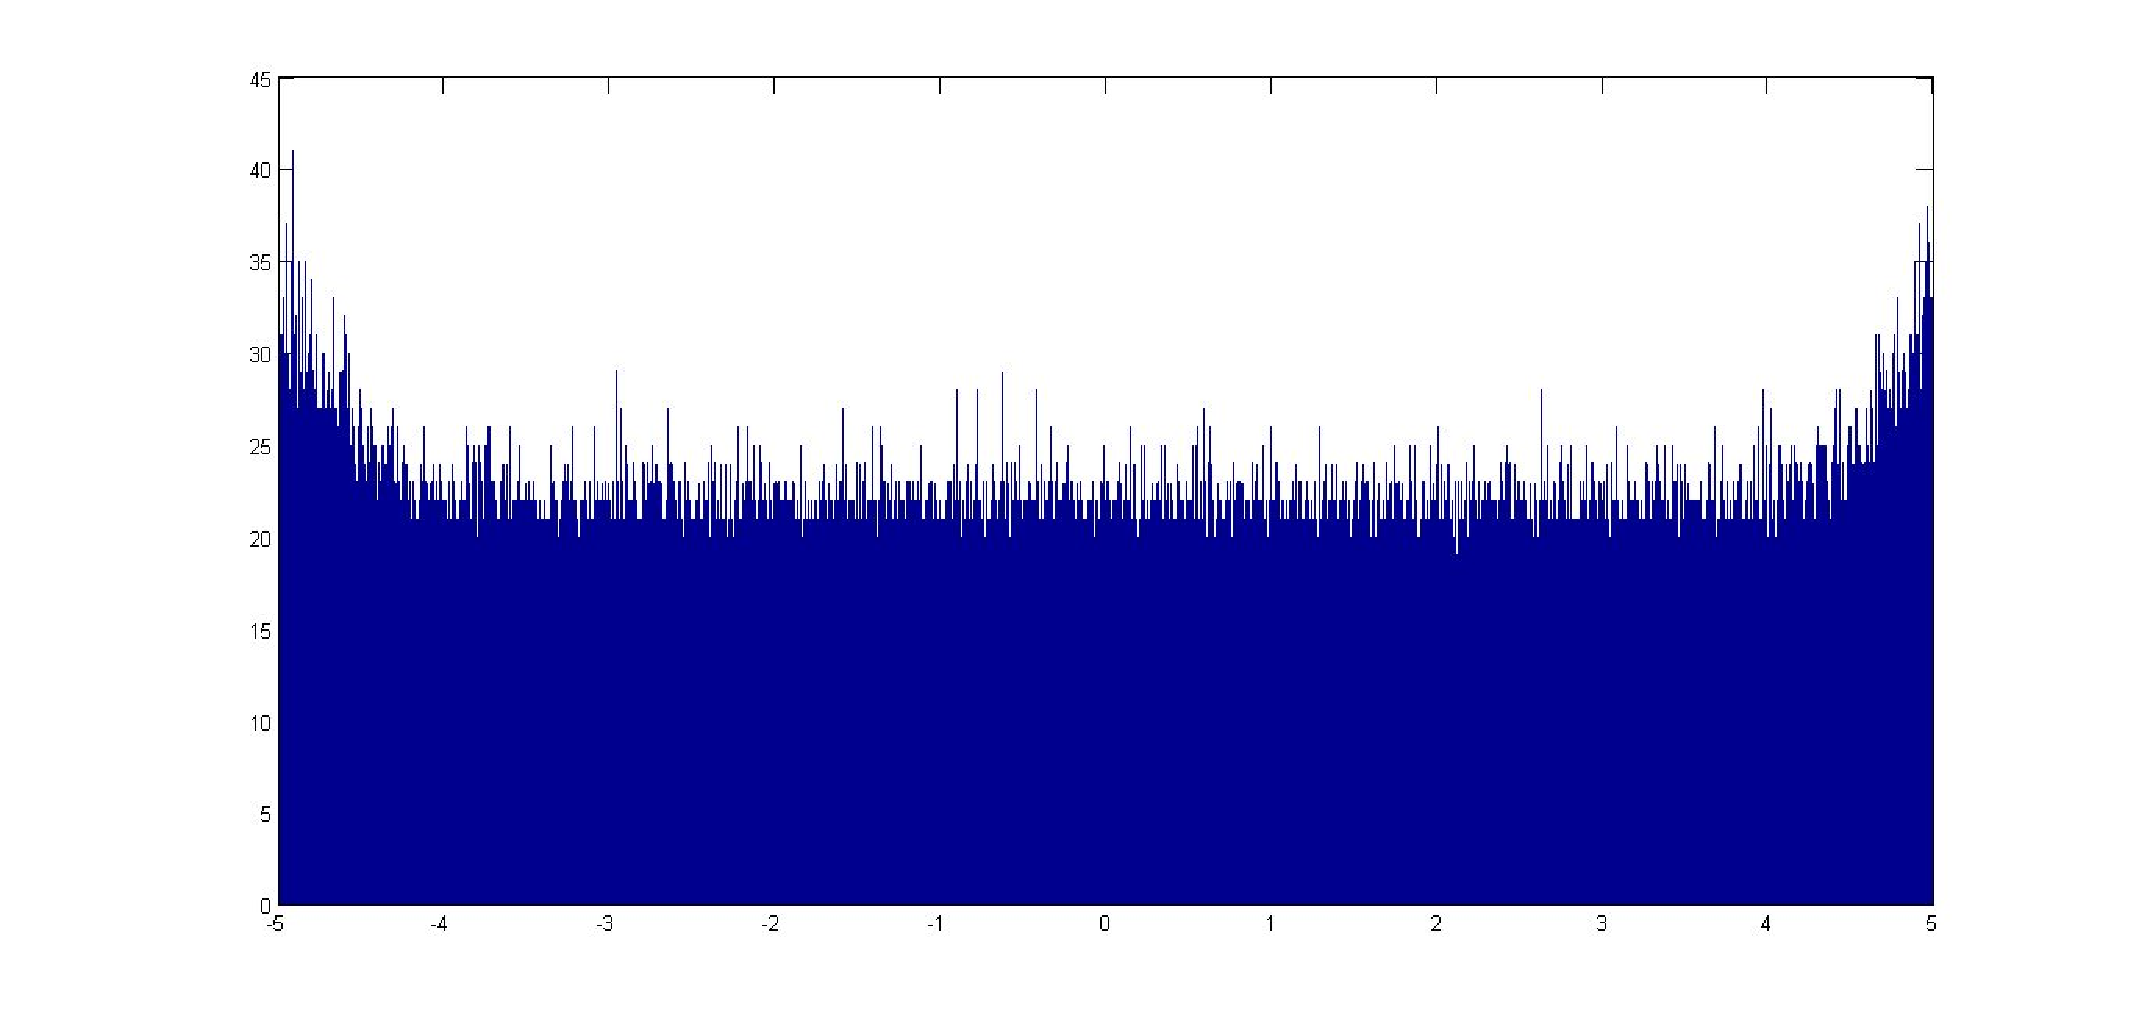
\includegraphics[width=0.45\textwidth]{c_n_20M_1__5_5_2}}
\quad
\subfloat[Generowanie z rozkładem jednostajnym]{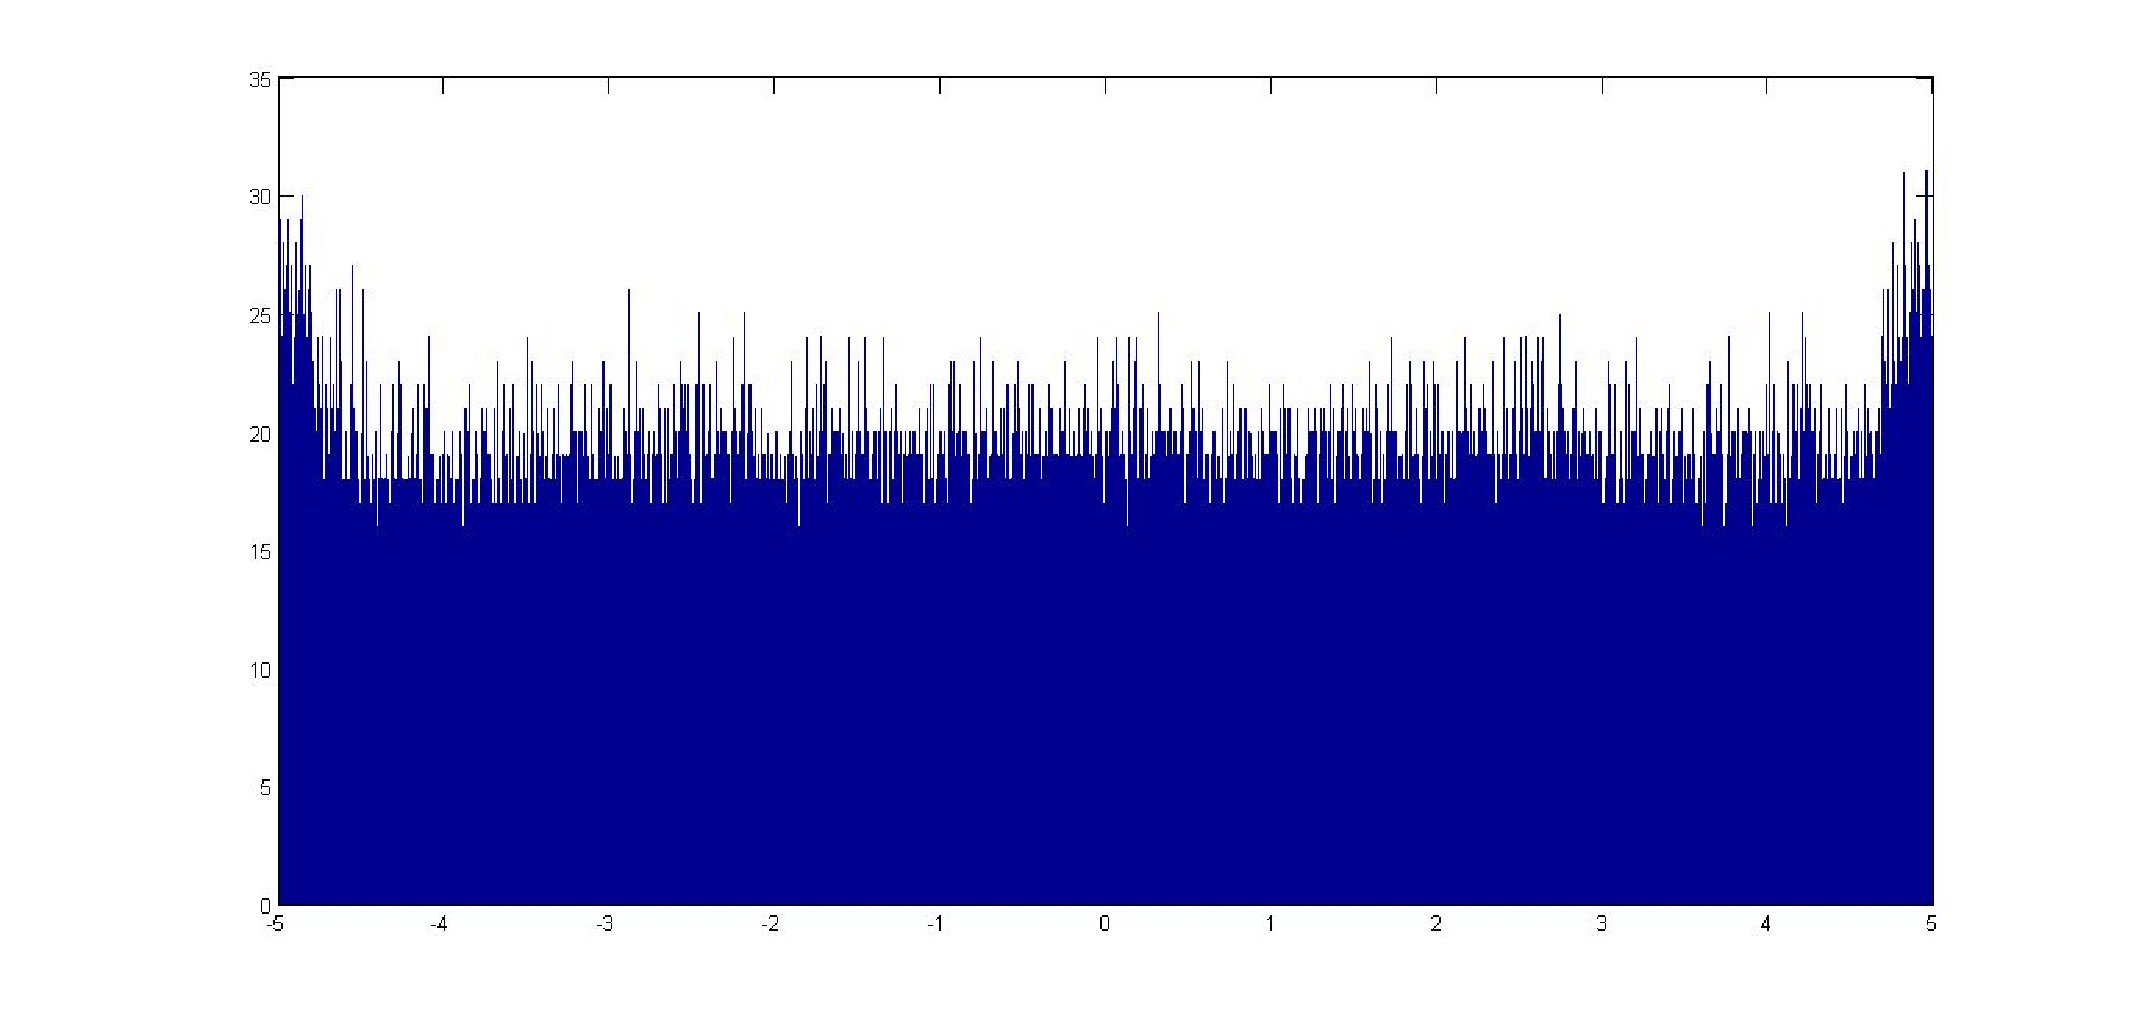
\includegraphics[width=0.45\textwidth]{c_j_2M_1__5_5}}
\caption{Rozkład prawdopodobieństwa punktów; 1 wymiar}
\end{figure}

\begin{figure}[H]
\centering
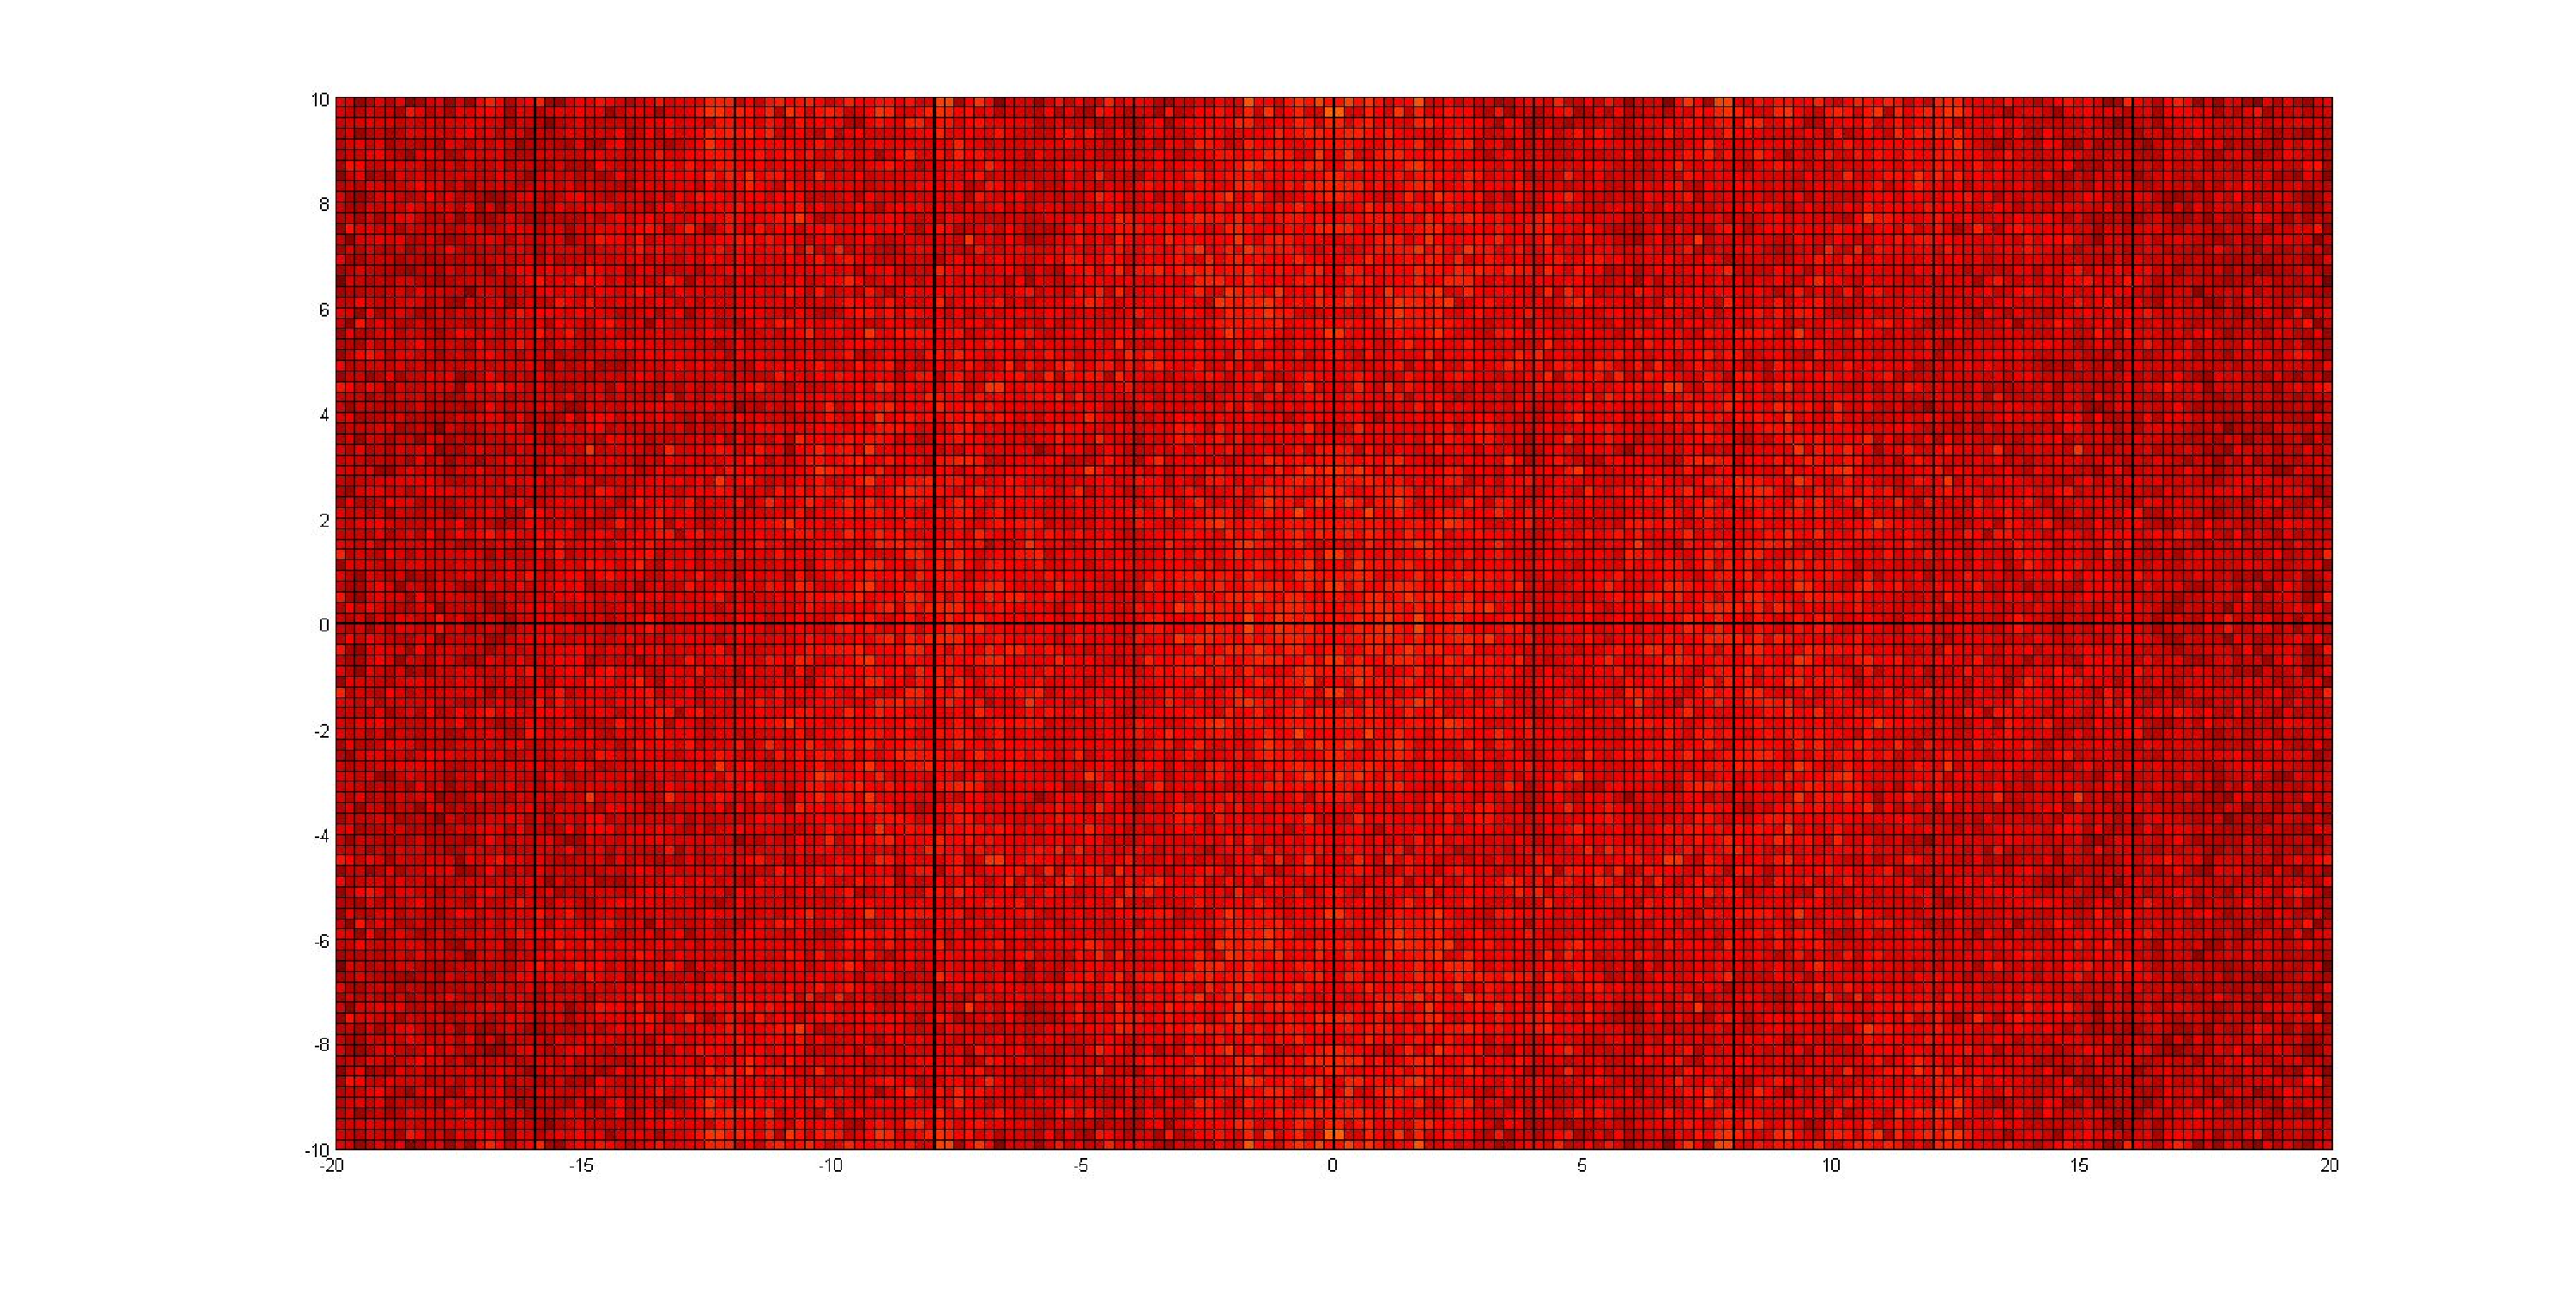
\includegraphics[width=\textwidth]{c_n_10M_2__20_20__10_10_4}
\caption{Rozkład prawdopodobieństwa punktów; 2 wymiary; generowanie z rozkładem normalnym}
\end{figure}

\subsubsection*{Rzutowanie}
Zgodnie z przewidywaniami największe prawdopodobieństwo wystąpienia punktu jest na ograniczeniu, co bardzo dobrze obrazuje rysunek \ref{bladzenie:rzutowanie2d}. Na rysunkach \ref{bladzenie:rzutowanie1dn} i \ref{bladzenie:rzutowanie1dj} zakres osi~Y został zmniejszony do odpowiednio $[30000;60000]$ oraz $[70000;140000]$, aby uwypuklić interesujące efekty. W związku z tym, wartości przedziałów brzegowych nie są widoczne - były o kilka rzędów wielkości większe od pozostałych wartości.

Warto zwrócić uwagę na niespodziewane zjawisko - wartości przedziałów blisko ograniczeń są mniejsze, niż pozostałe. Oznacza to, że punkty w tych przedziałach występują z mniejszym prawdopodobieństwem, niż pozostałe. Wydawać by się mogło, że powinno być inaczej, ponieważ podczas symulacji punkty często są rzutowane na ograniczenie. Dodatkowo, w rozkładzie jednostajnym widać, że istnieją przedziały, w~których punkty występują z~większym prawdopodobieństwem. Autorowi nie udało się formalnie uzasadnić tego zjawiska. Intuicja prowadzi do hipotezy, że punkty, które znalazły się poza ograniczeniem, bez naprawy po kilku iteracjach zapełniałyby "dołek". Naprawa natomiast sprawia, że cała dalsza symulacja zostaje niejako przesunięta. W~ten sposób powstaje "górka" w~rozkładzie jednostajnym. Brak górki w rozkładzie normalnym można tłumaczyć charakterystyką samego rozkładu - spadek prawdopodobieństwa wraz z oddalaniem się od wartości oczekiwanej.

\begin{figure}[H]
\centering
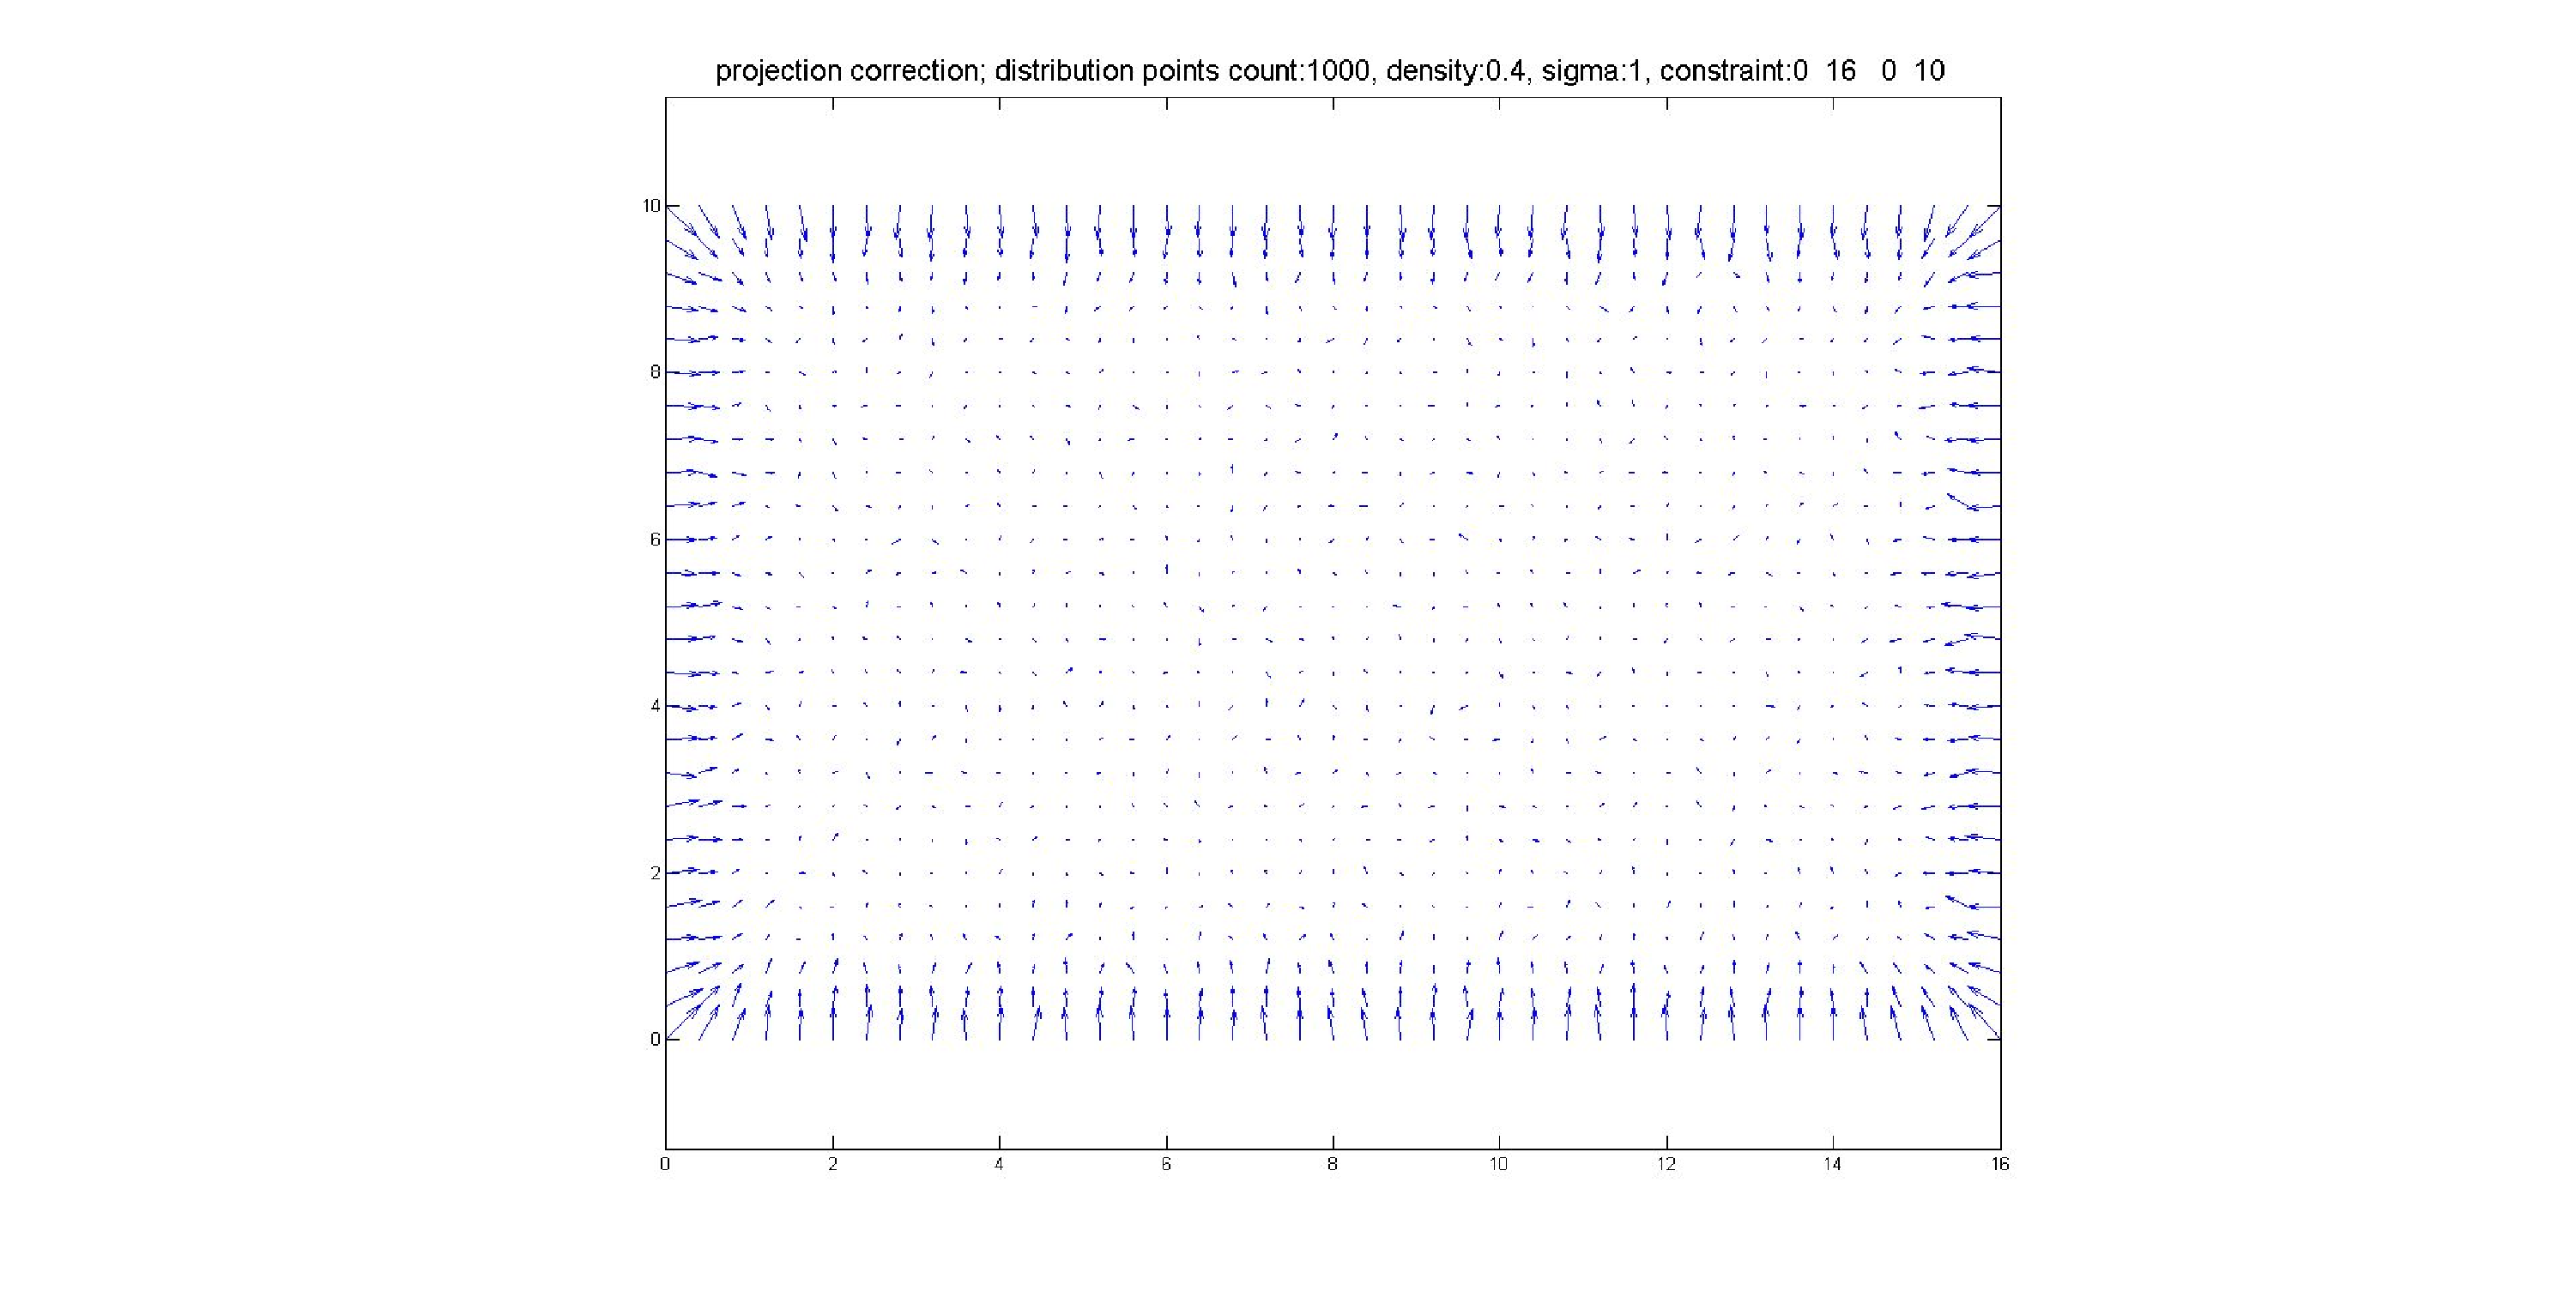
\includegraphics[width=\textwidth]{projection2dprzesuniecie}
\caption{Wartość oczekiwana punktu}
\end{figure}

\begin{figure}[H]
\centering
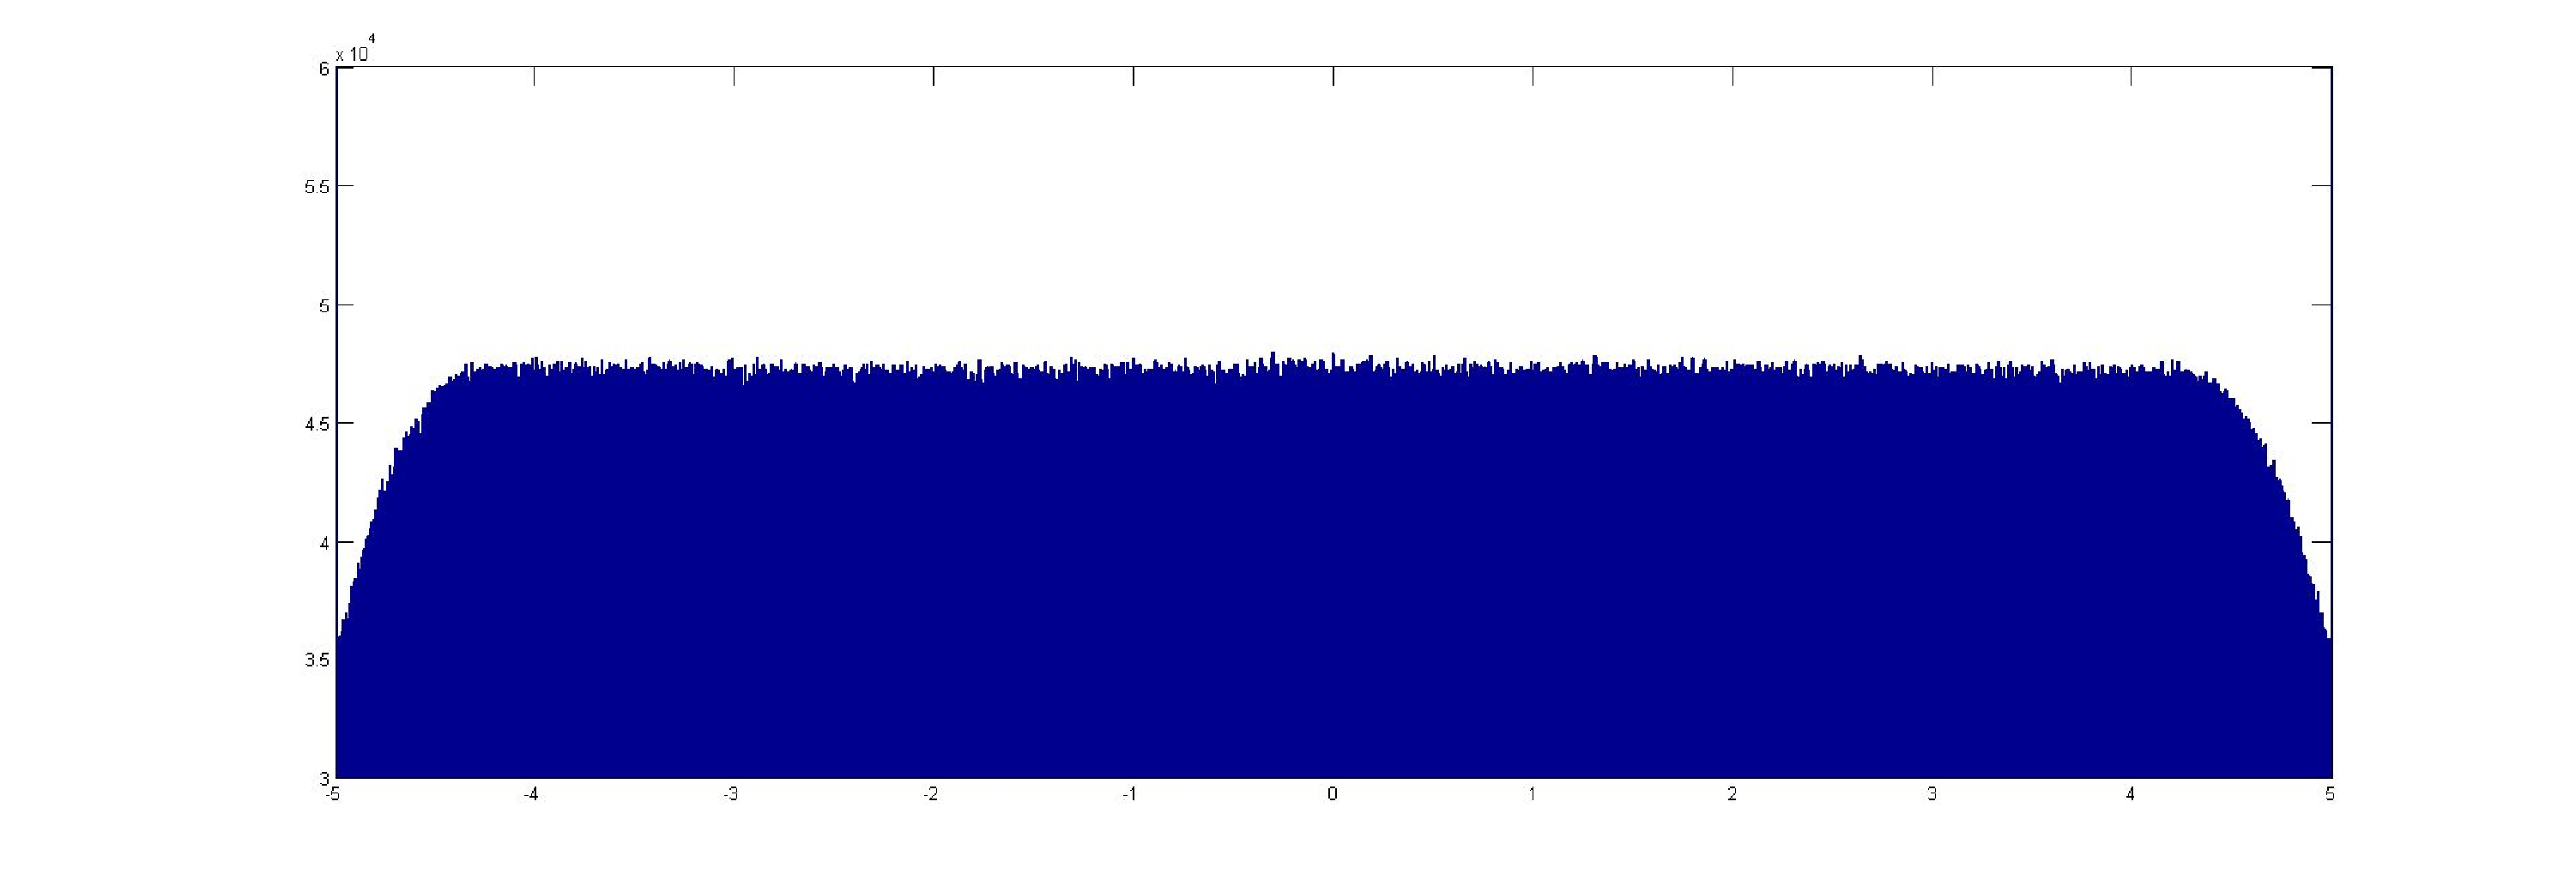
\includegraphics[width=\textwidth]{p_n_50M_1__5_5}
\caption{Rozkład prawdopodobieństwa punktów; 1 wymiar; generowanie z rozkładem normalnym}
\label{bladzenie:rzutowanie1dn}
\end{figure}

\begin{figure}[H]
\centering
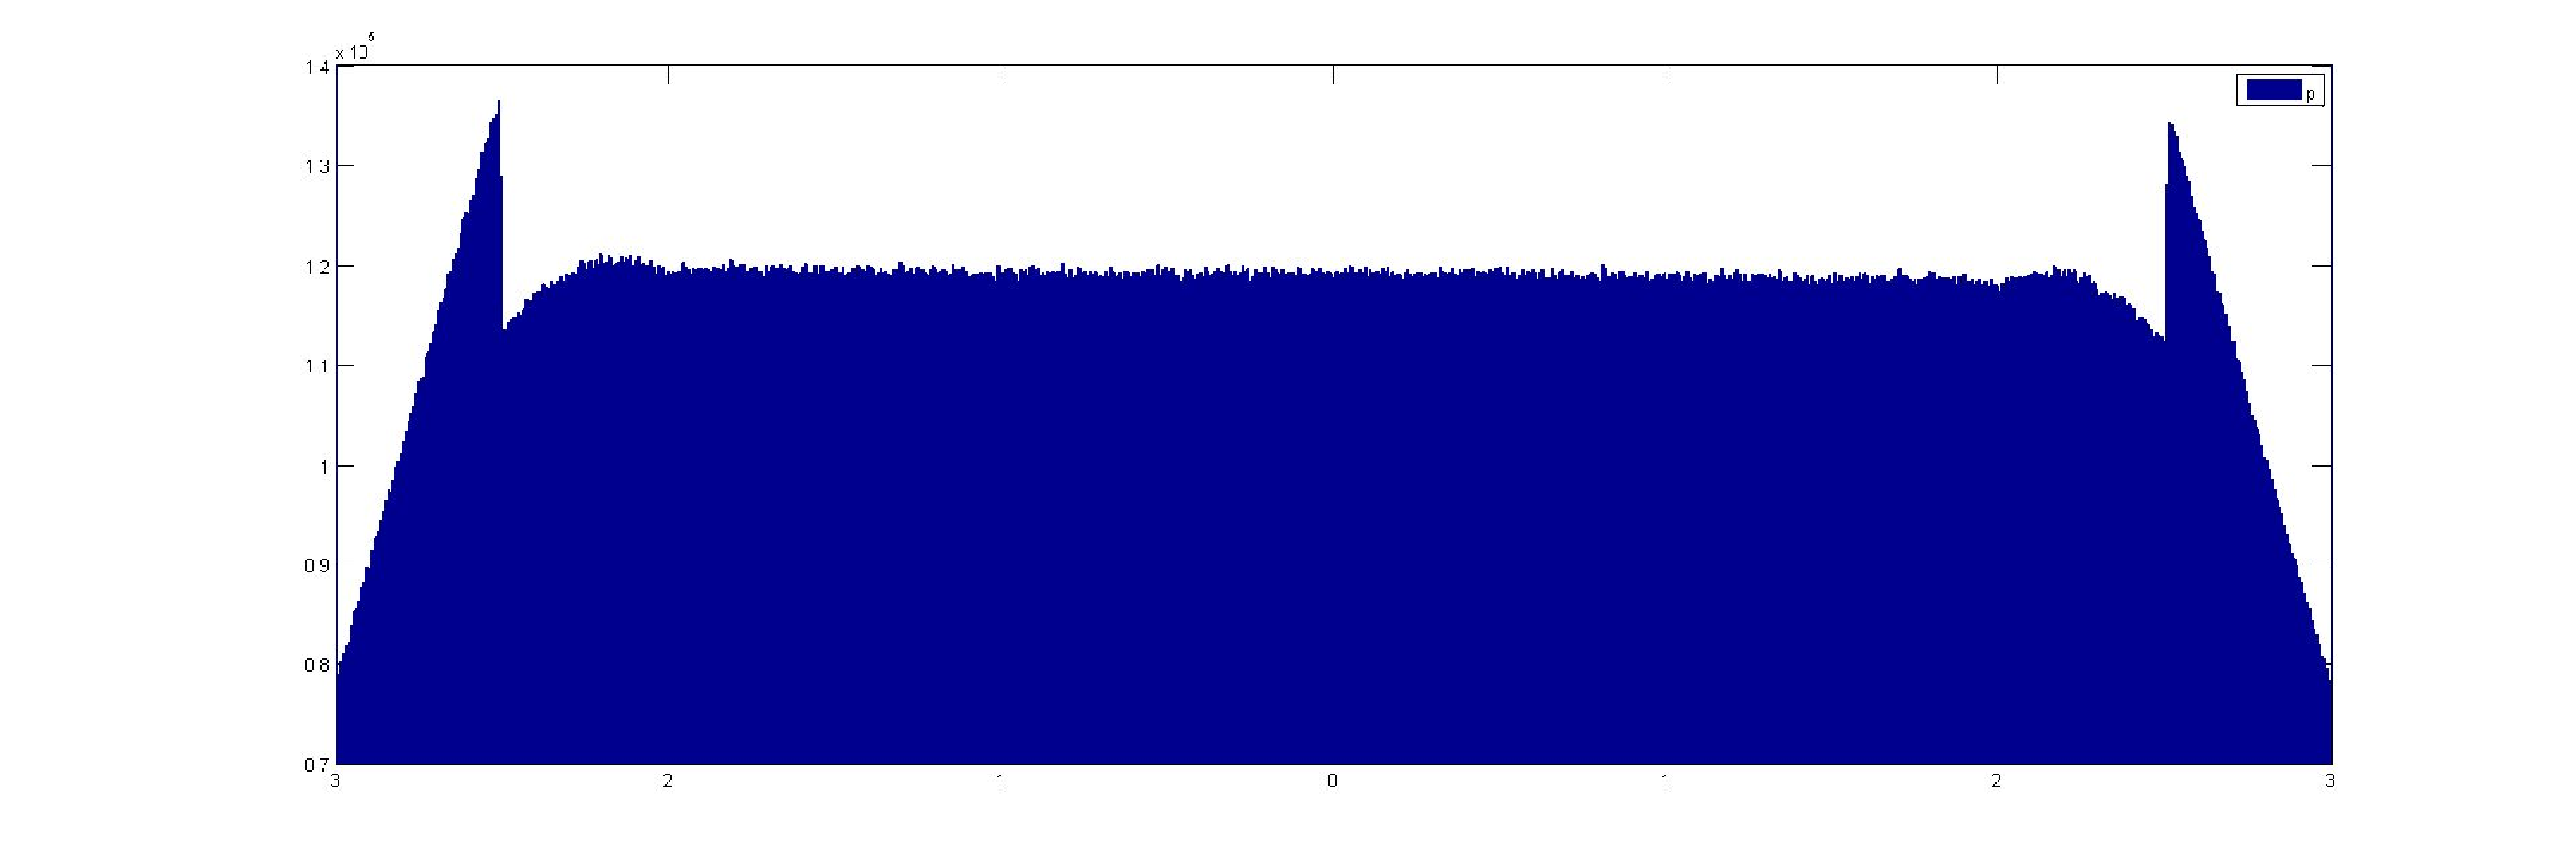
\includegraphics[width=\textwidth]{p_j_100M_1__3_3}
\caption{Rozkład prawdopodobieństwa punktów; 1 wymiar; generowanie z rozkładem jednostajnym}
\label{bladzenie:rzutowanie1dj}
\end{figure}

\begin{figure}[H]
\centering
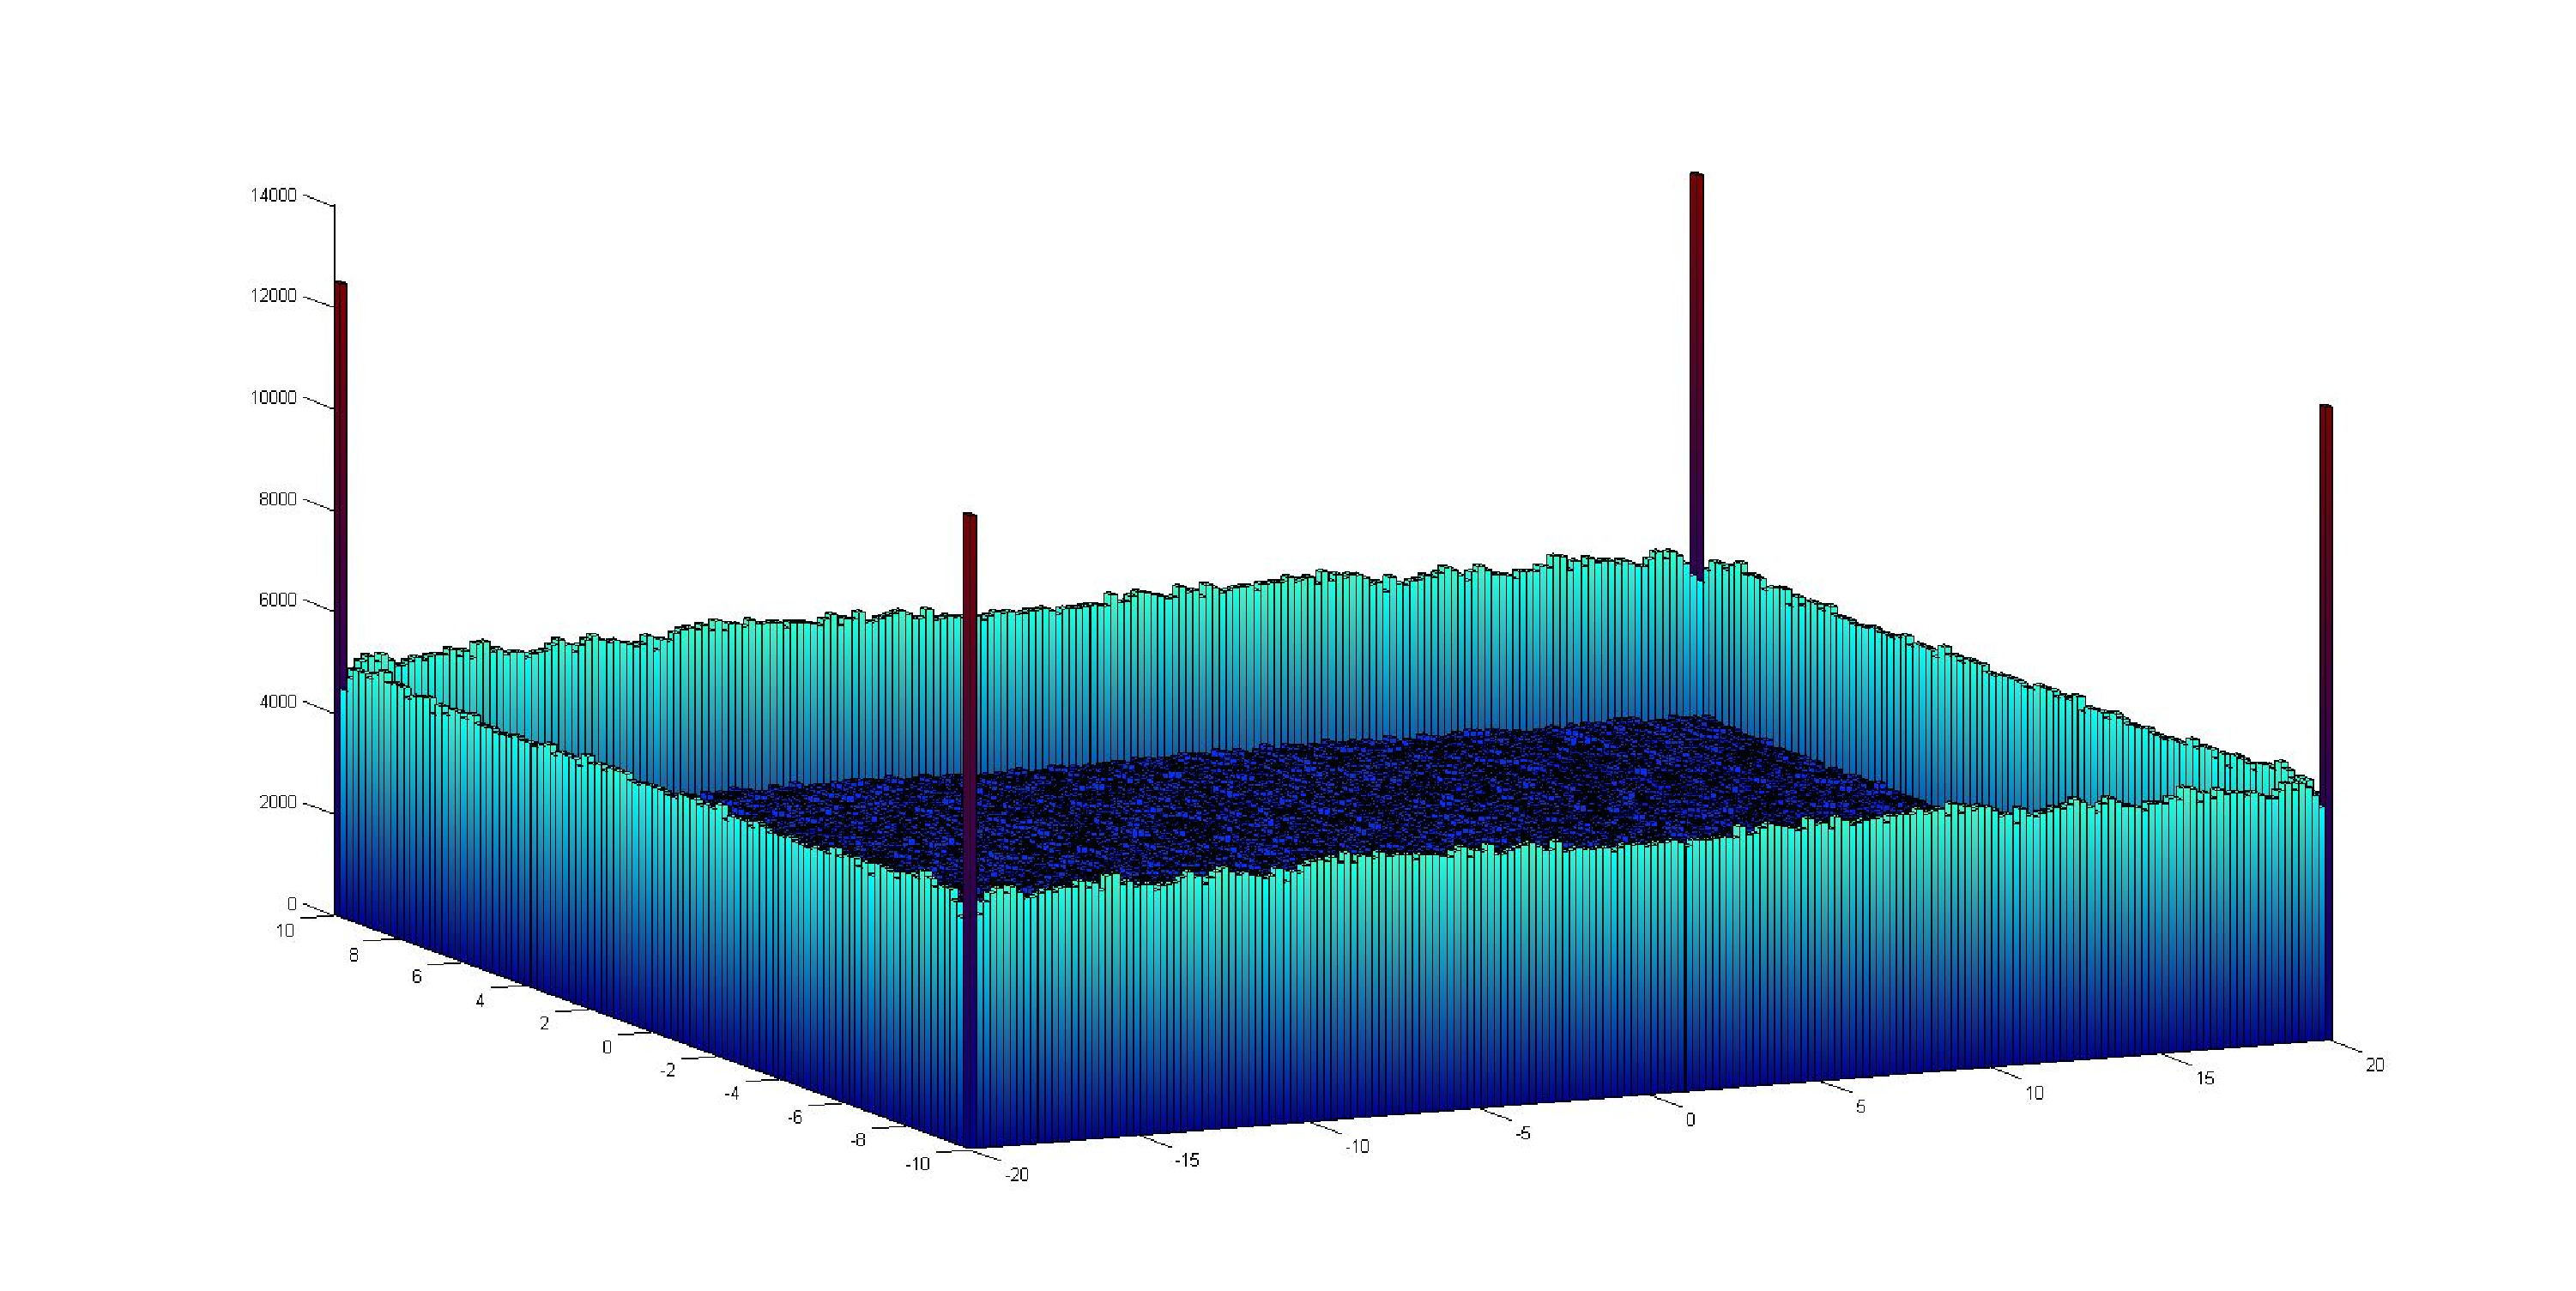
\includegraphics[width=\textwidth]{p_n_10M_2__20_20__10_10_4_2}
\caption{Rozkład prawdopodobieństwa punktów; 2 wymiary; generowanie z rozkładem normalnym}
\label{bladzenie:rzutowanie2d}
\end{figure}

\subsubsection*{Reinicjacja}
Wykres wartości oczekiwanych jest mało czytelny, ponieważ wartości przesunięć są duże. Ma w tym udział reinicjacja, która przesuwa część punktów na środek przestrzeni przeszukiwań.

Histogramy nie ukazują nic nadzwyczajnego, ponieważ łatwo zauważyć pik związany z reinicjacją oraz wartości histogramu malejące wraz ze zbliżaniem się do ograniczeń. Warto jednak zwrócić uwagę na 2 fakty.

Pierwsze spostrzeżenie, to kształt histogramu. Zarówno dla rozkładu jednostajnego, jak i normalnego w jednym wymiarze jest on stożkowy. Łuk można zauważyć tylko blisko punktu środkowego, w pozostałej części spadek jest liniowy. Brakuje charakterystycznego, gaussowskiego przegięcia. Sytuacja jest ciekawsza, gdy występuje więcej wymiarów. Widać wówczas przegięcie (Rysunek \ref{bladzenie:reinicjacja2ds}). Dokładniejsze badania pokazały, że przegięcie nie występuje tylko na jednym wymiarze - tym, który jest relatywnie najkrótszy. Celowo jest użyte słowo relatywnie, ponieważ z~perspektywy błądzenia przypadkowego i~rozkładu normalnego trzeba brać pod uwagę parametr $\sigma$ - odchylenie standardowe. Wymiary o małym $\sigma$ będą relatywnie dłuższe od tych z dużym $\sigma$, ponieważ błądzenie będzie wykonywało mniejsze kroki.

Na rysunku \ref{bladzenie:reinicjacja1dj} można dostrzec też dwa uskoki, które związane są z pikiem w punkcie~$0$ oraz charakterystyką rozkładu jednostajnego.

\begin{figure}[H]
\centering
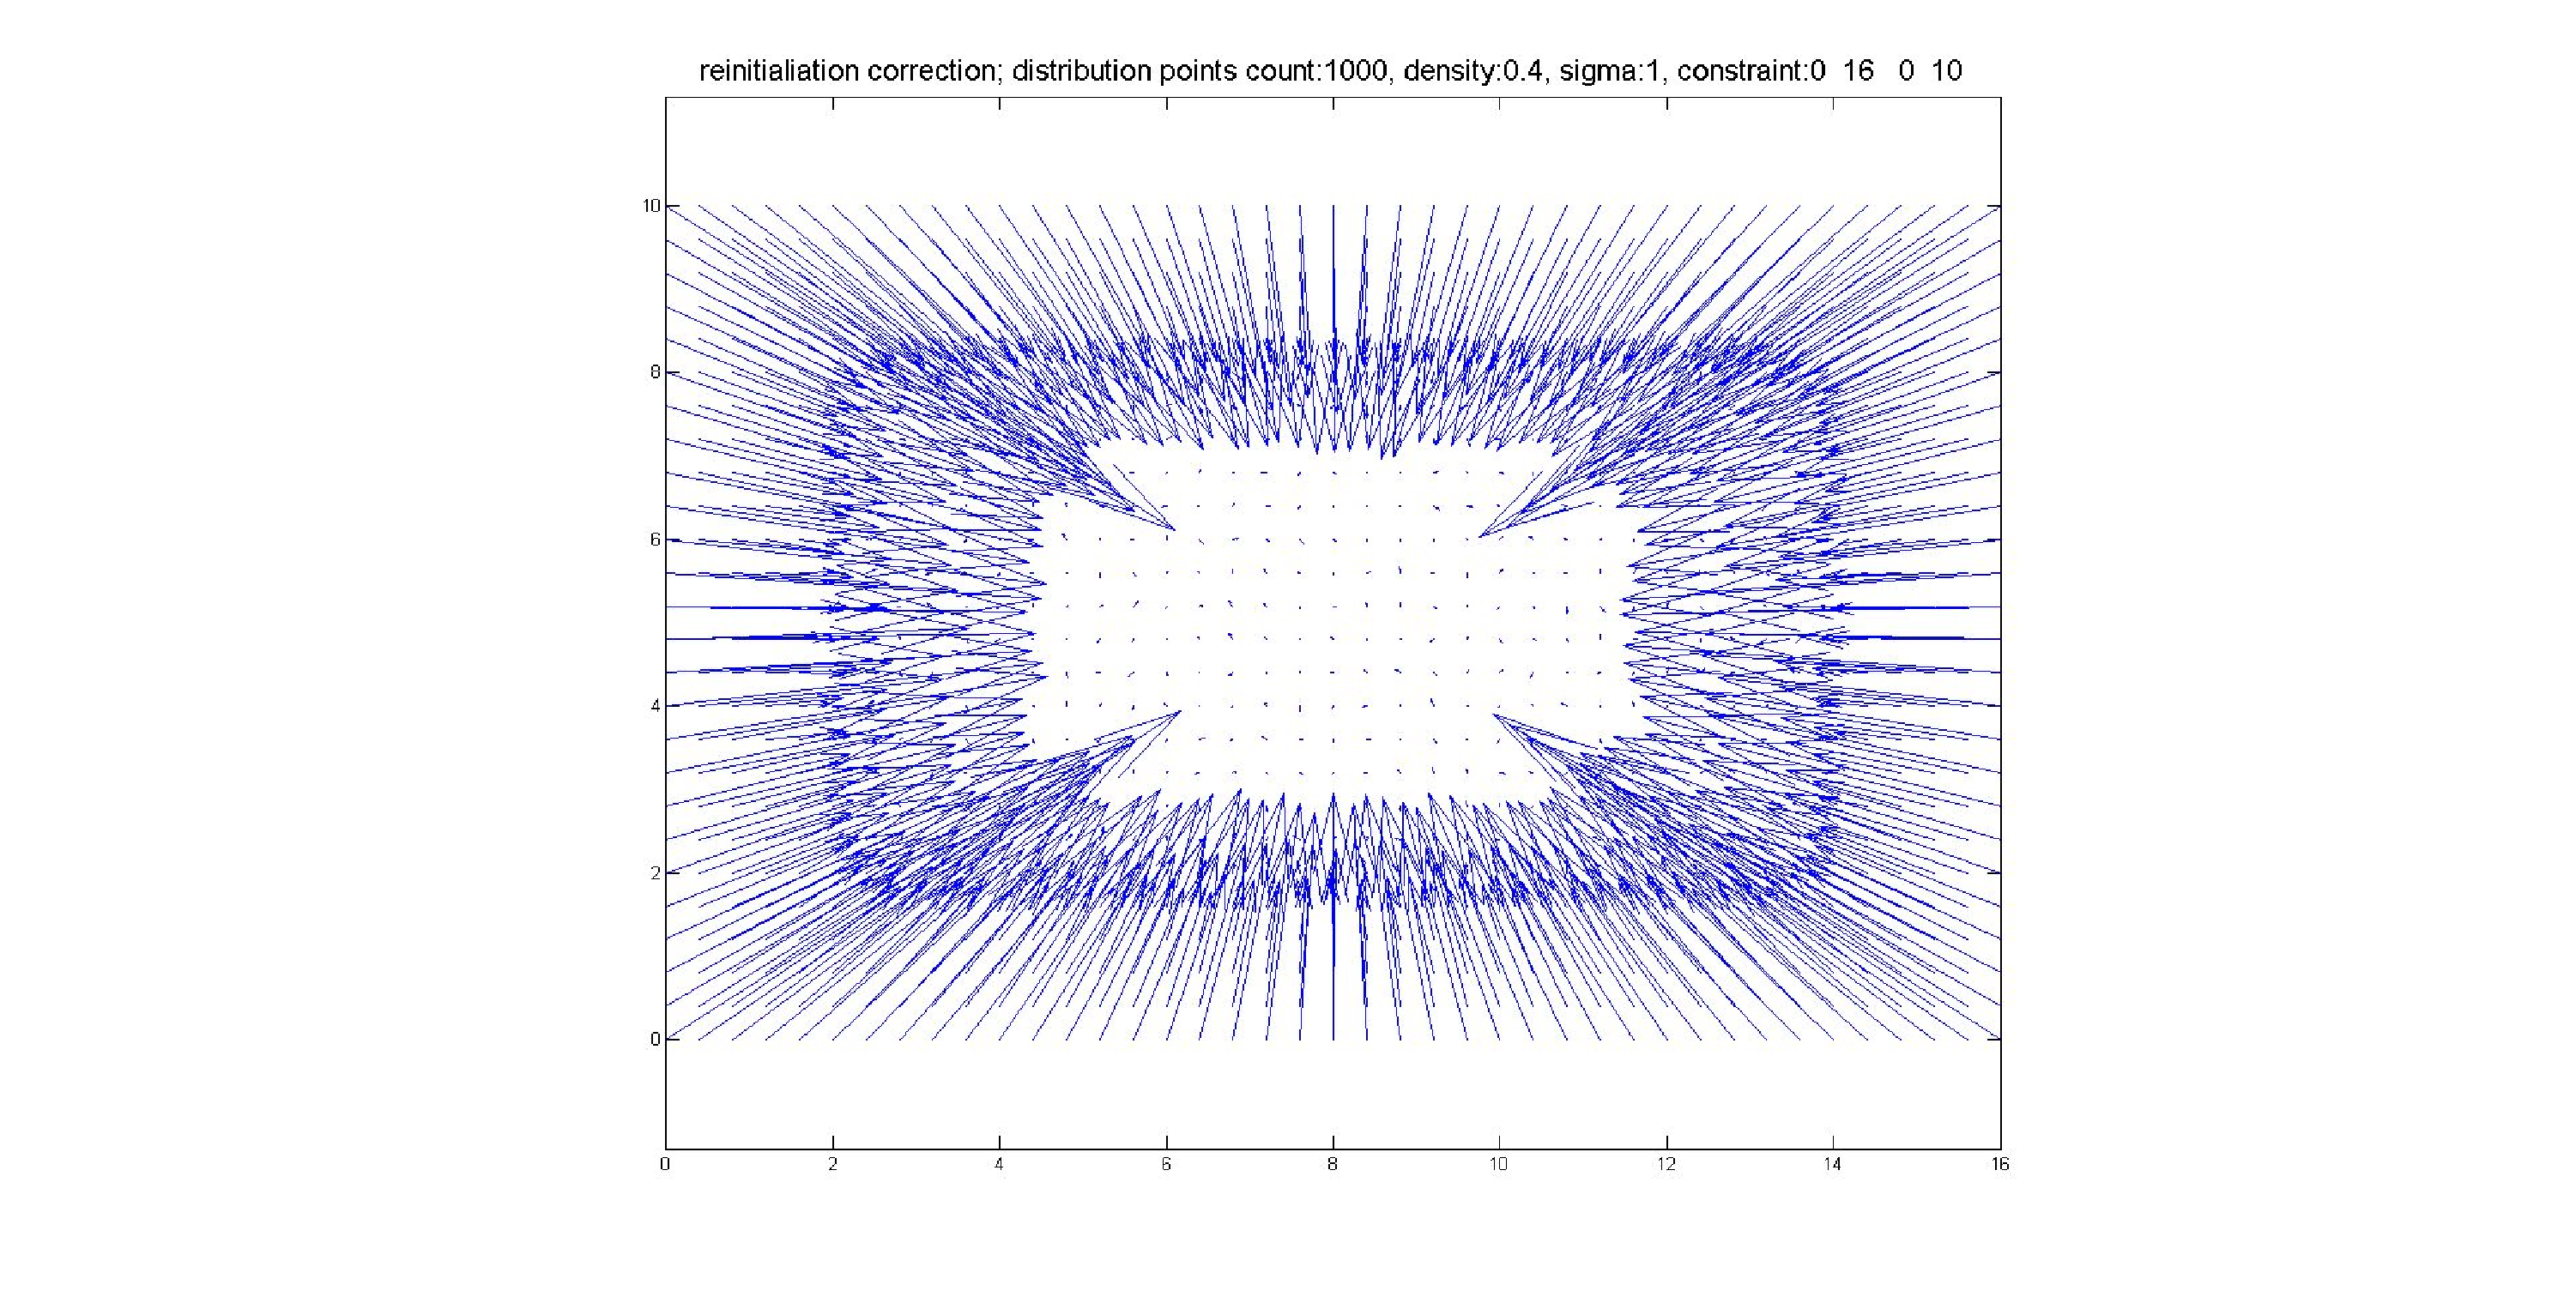
\includegraphics[width=\textwidth]{reinitialization2dprzesuniecie}
\caption{Wartość oczekiwana punktu}
\end{figure}

\begin{figure}[H]
\centering
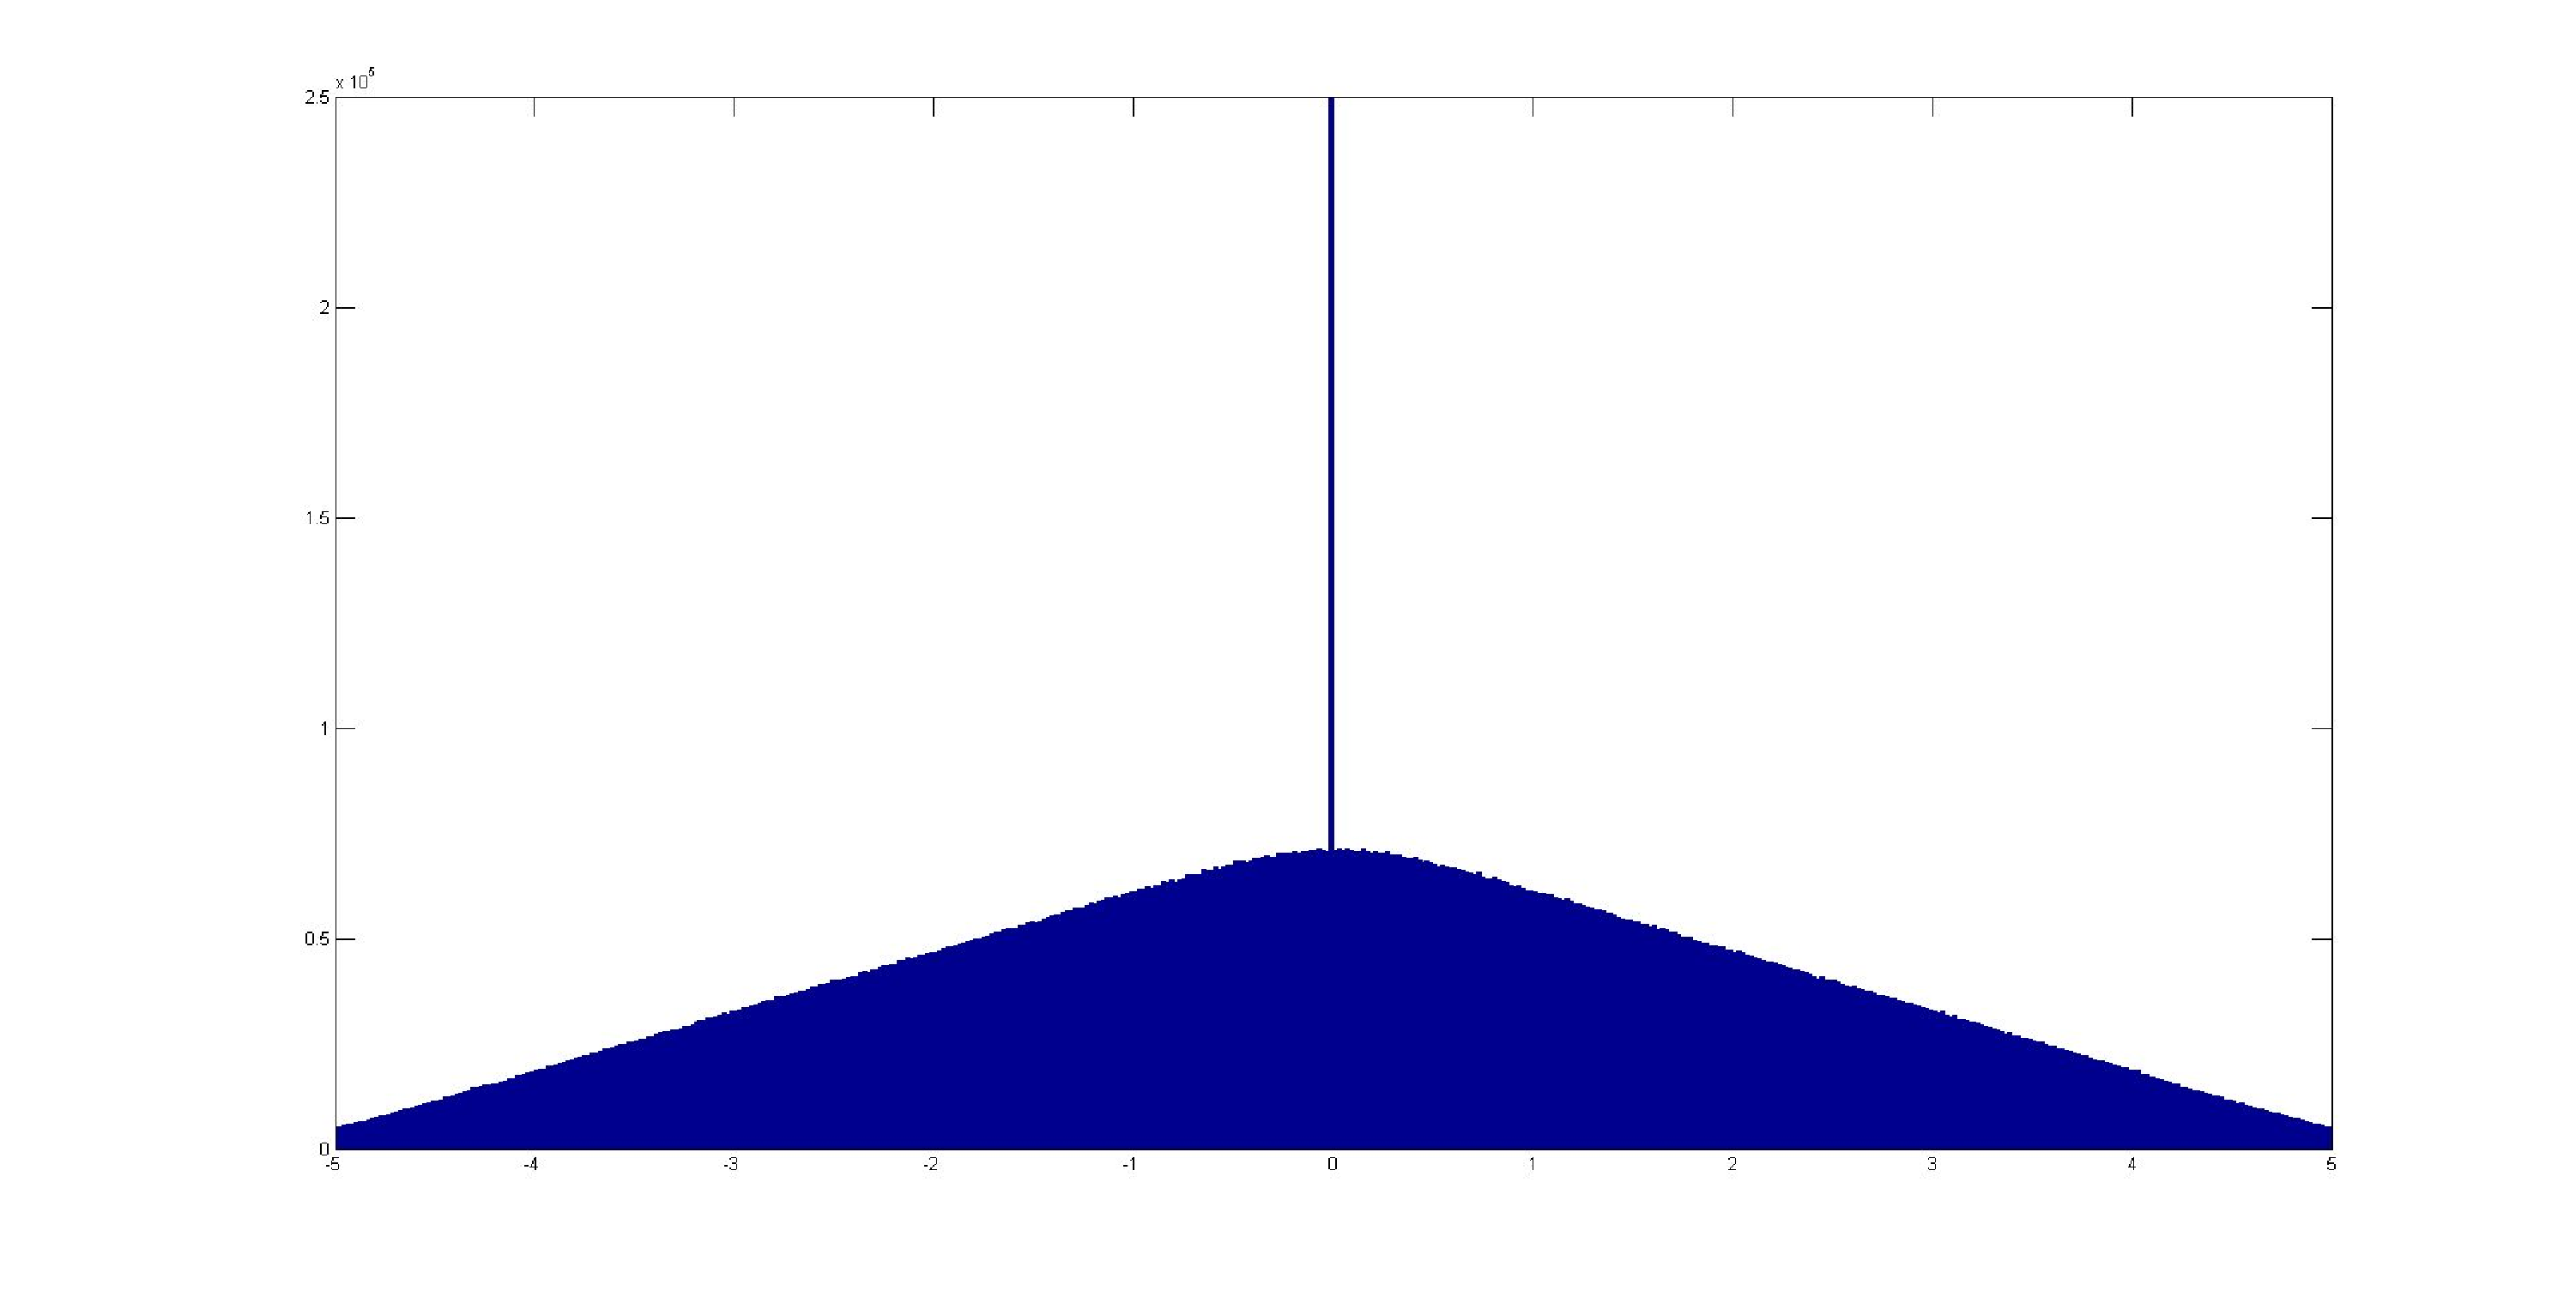
\includegraphics[width=\textwidth]{ri_n_20M_1__5_5}
\caption{Rozkład prawdopodobieństwa punktów; 1 wymiar; generowanie z rozkładem normalnym}
\end{figure}

\begin{figure}[H]
\centering
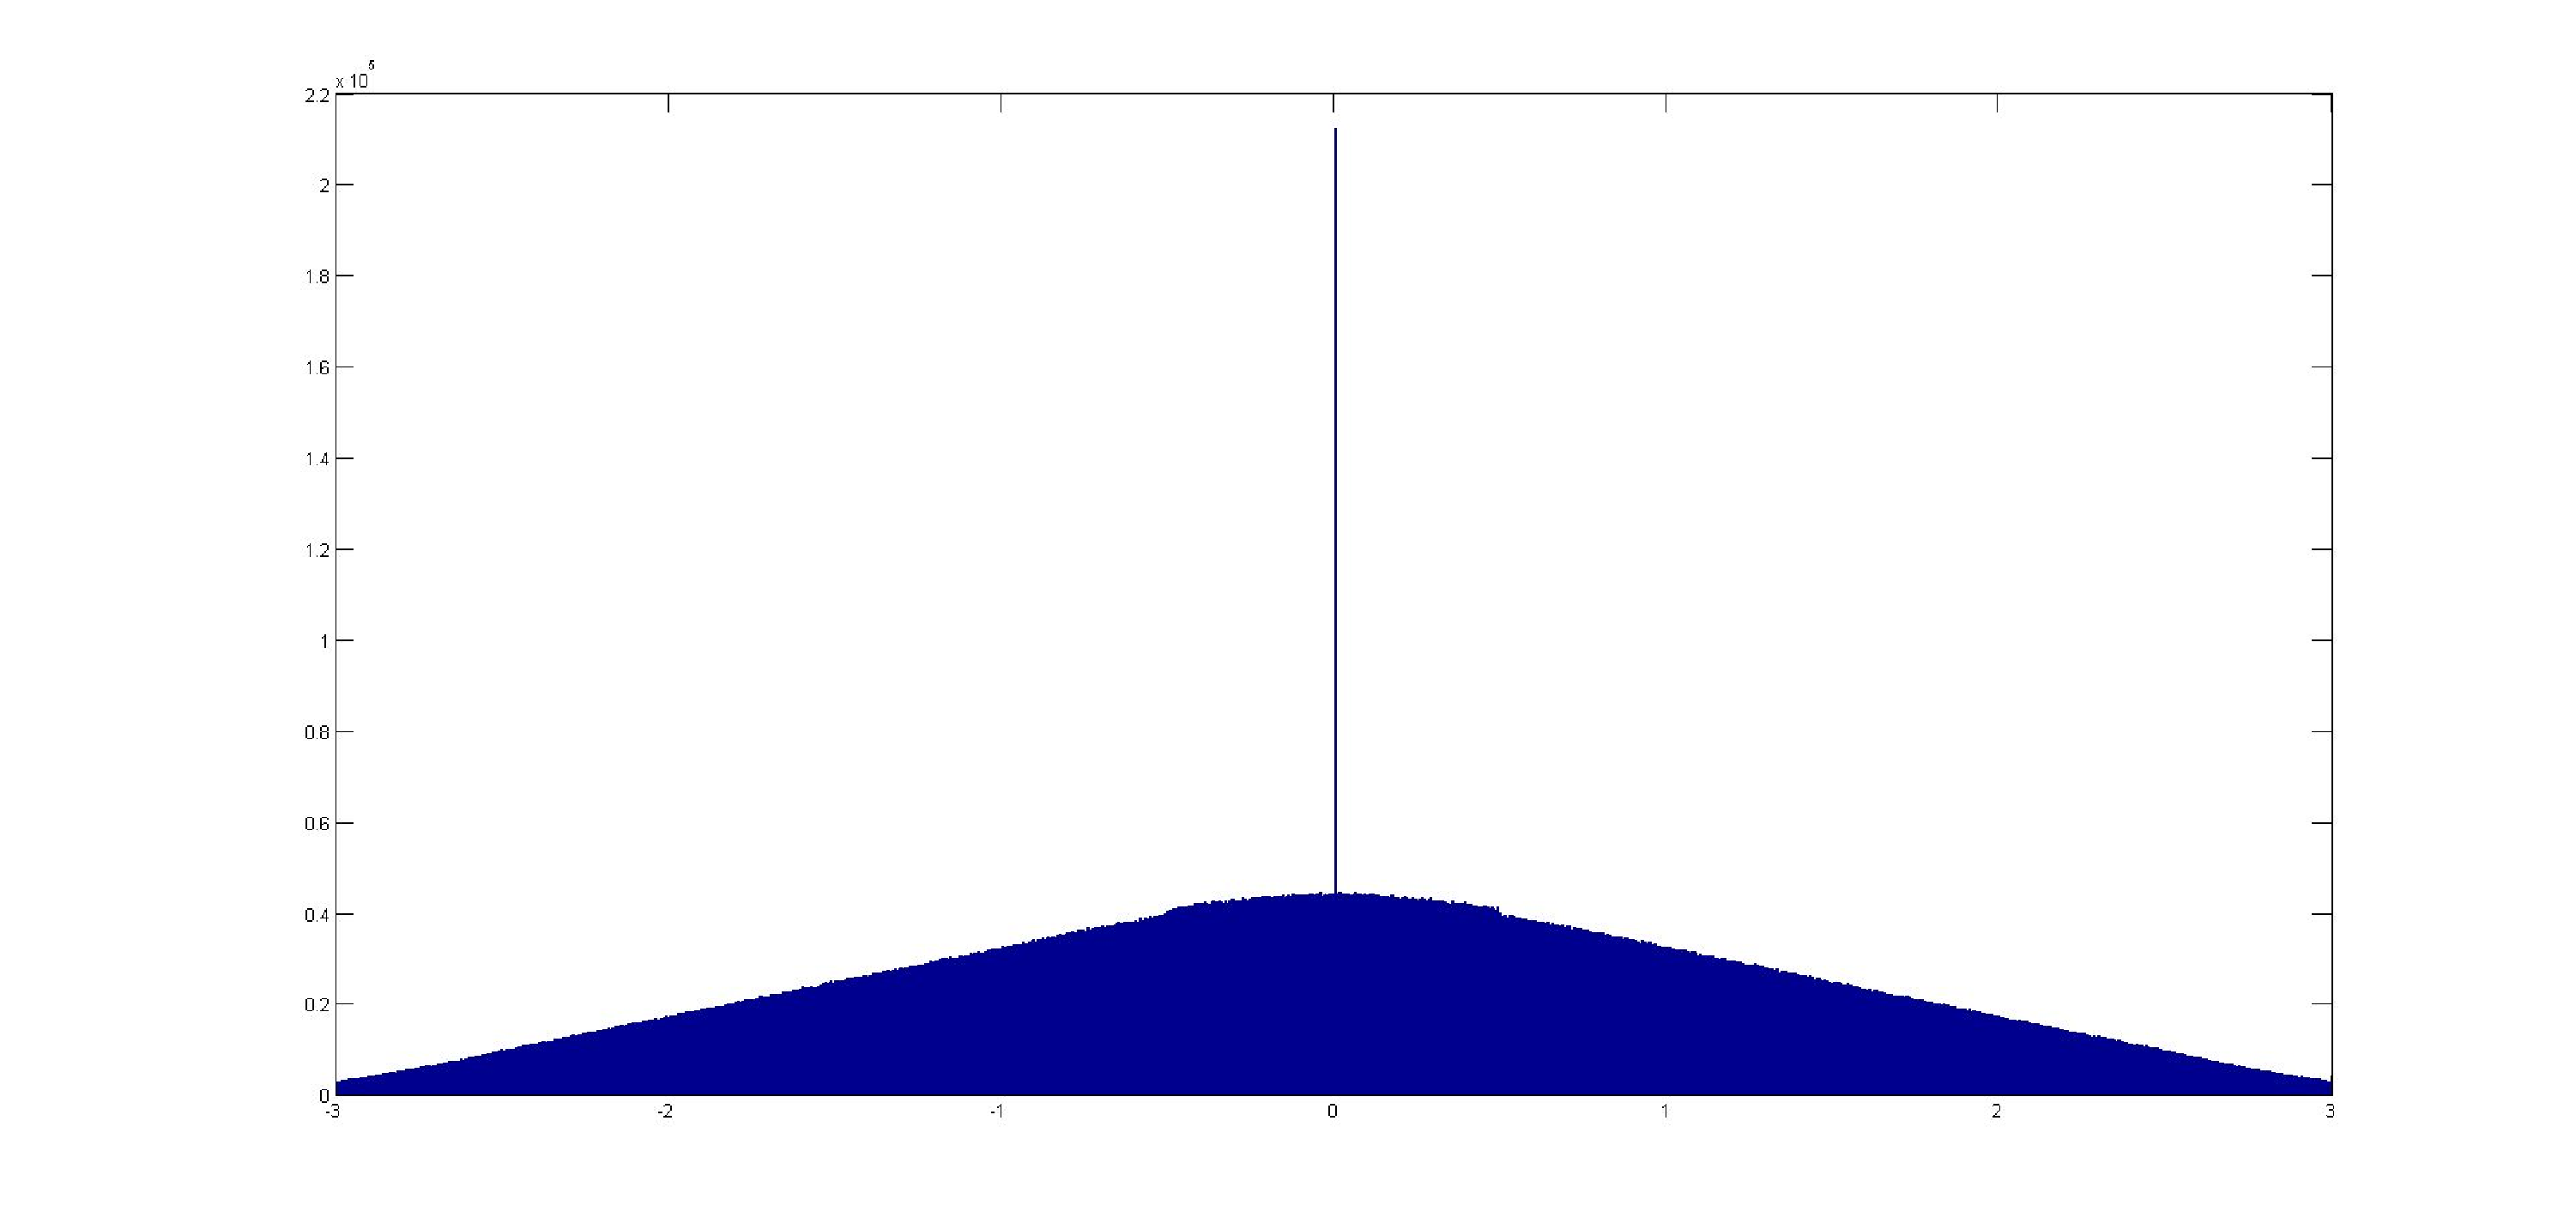
\includegraphics[width=\textwidth]{ri_j_20M_1__3_3}
\caption{Rozkład prawdopodobieństwa punktów; 1 wymiar; generowanie z rozkładem jednostajnym}
\label{bladzenie:reinicjacja1dj}
\end{figure}

\begin{figure}[H]
\centering
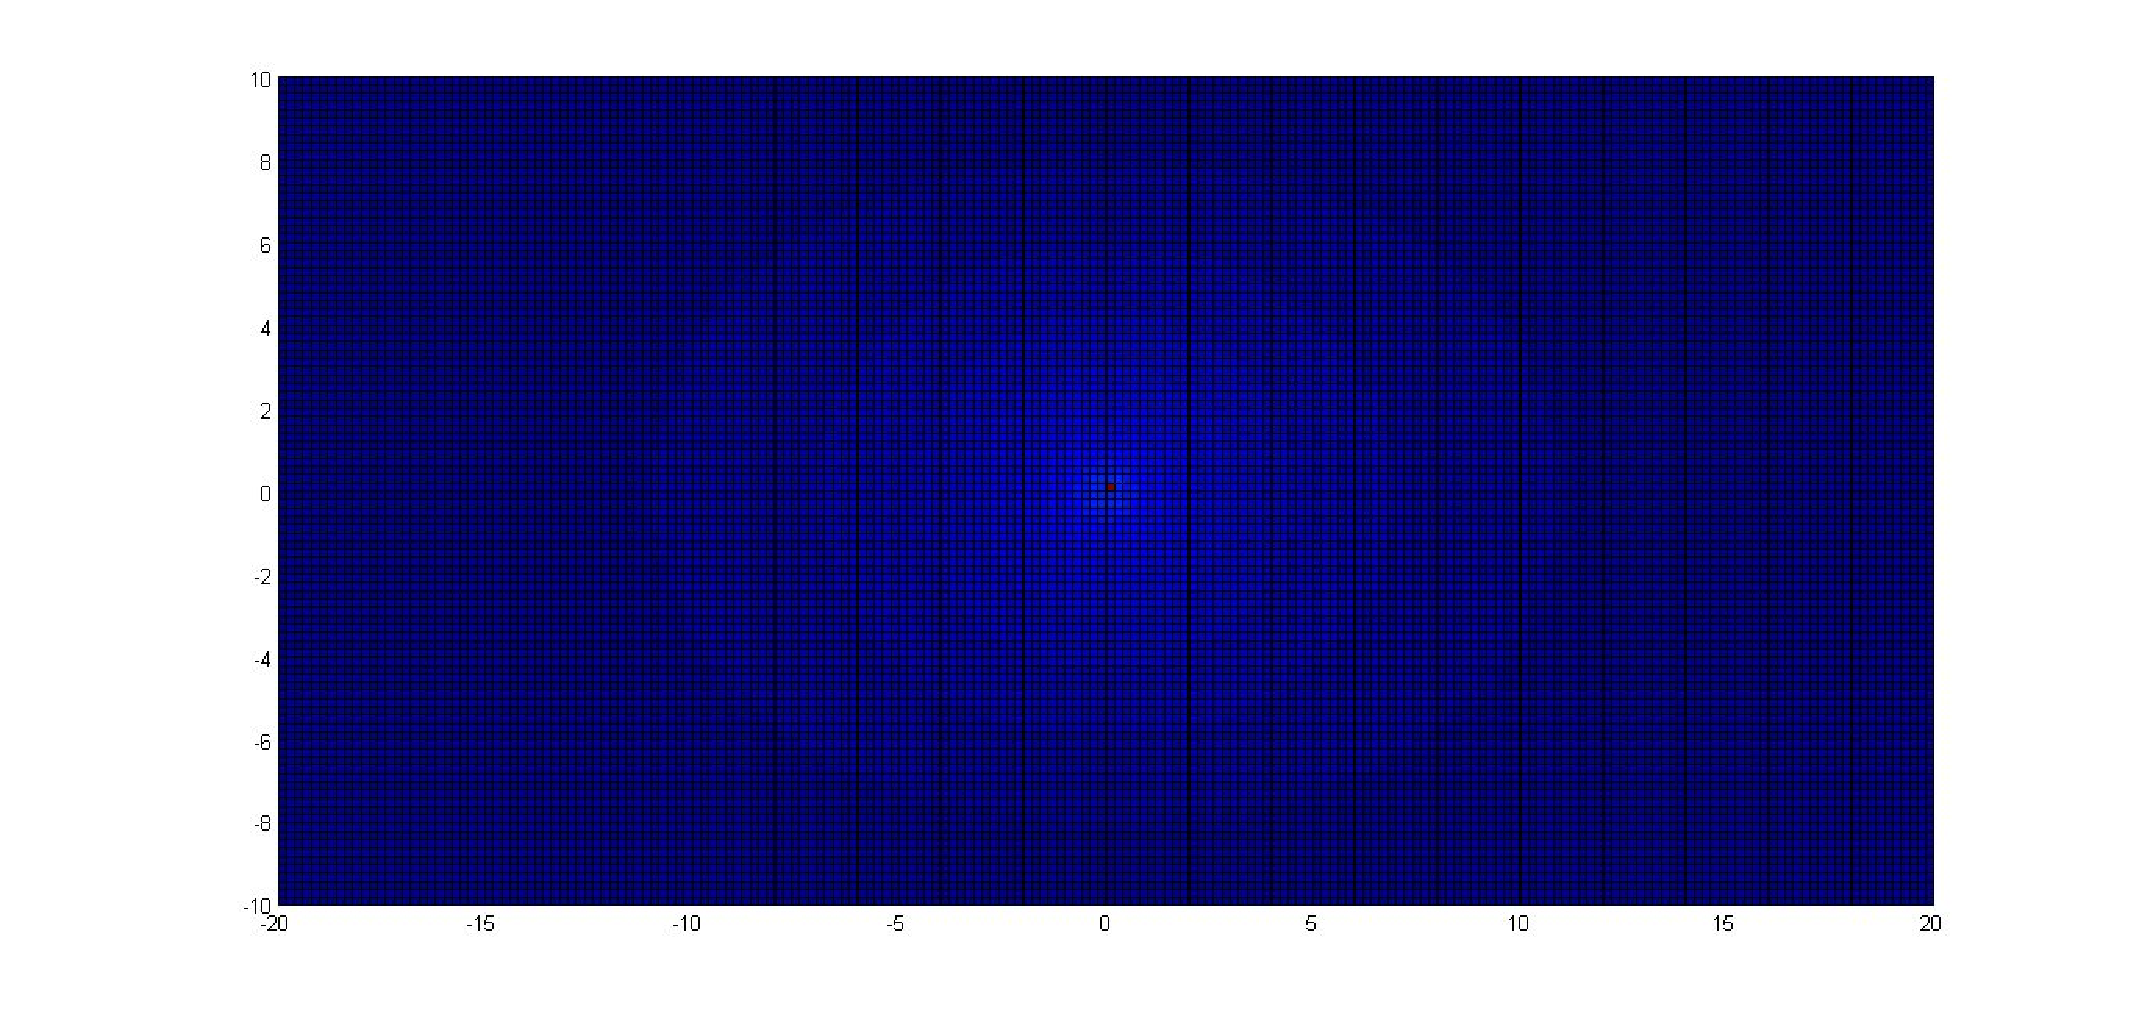
\includegraphics[width=\textwidth]{ri_n_10M_2__20_20__10_10_4}
\caption{Rozkład prawdopodobieństwa punktów; 2 wymiary; generowanie z rozkładem normalnym}
\end{figure}

\begin{figure}[H]
\centering
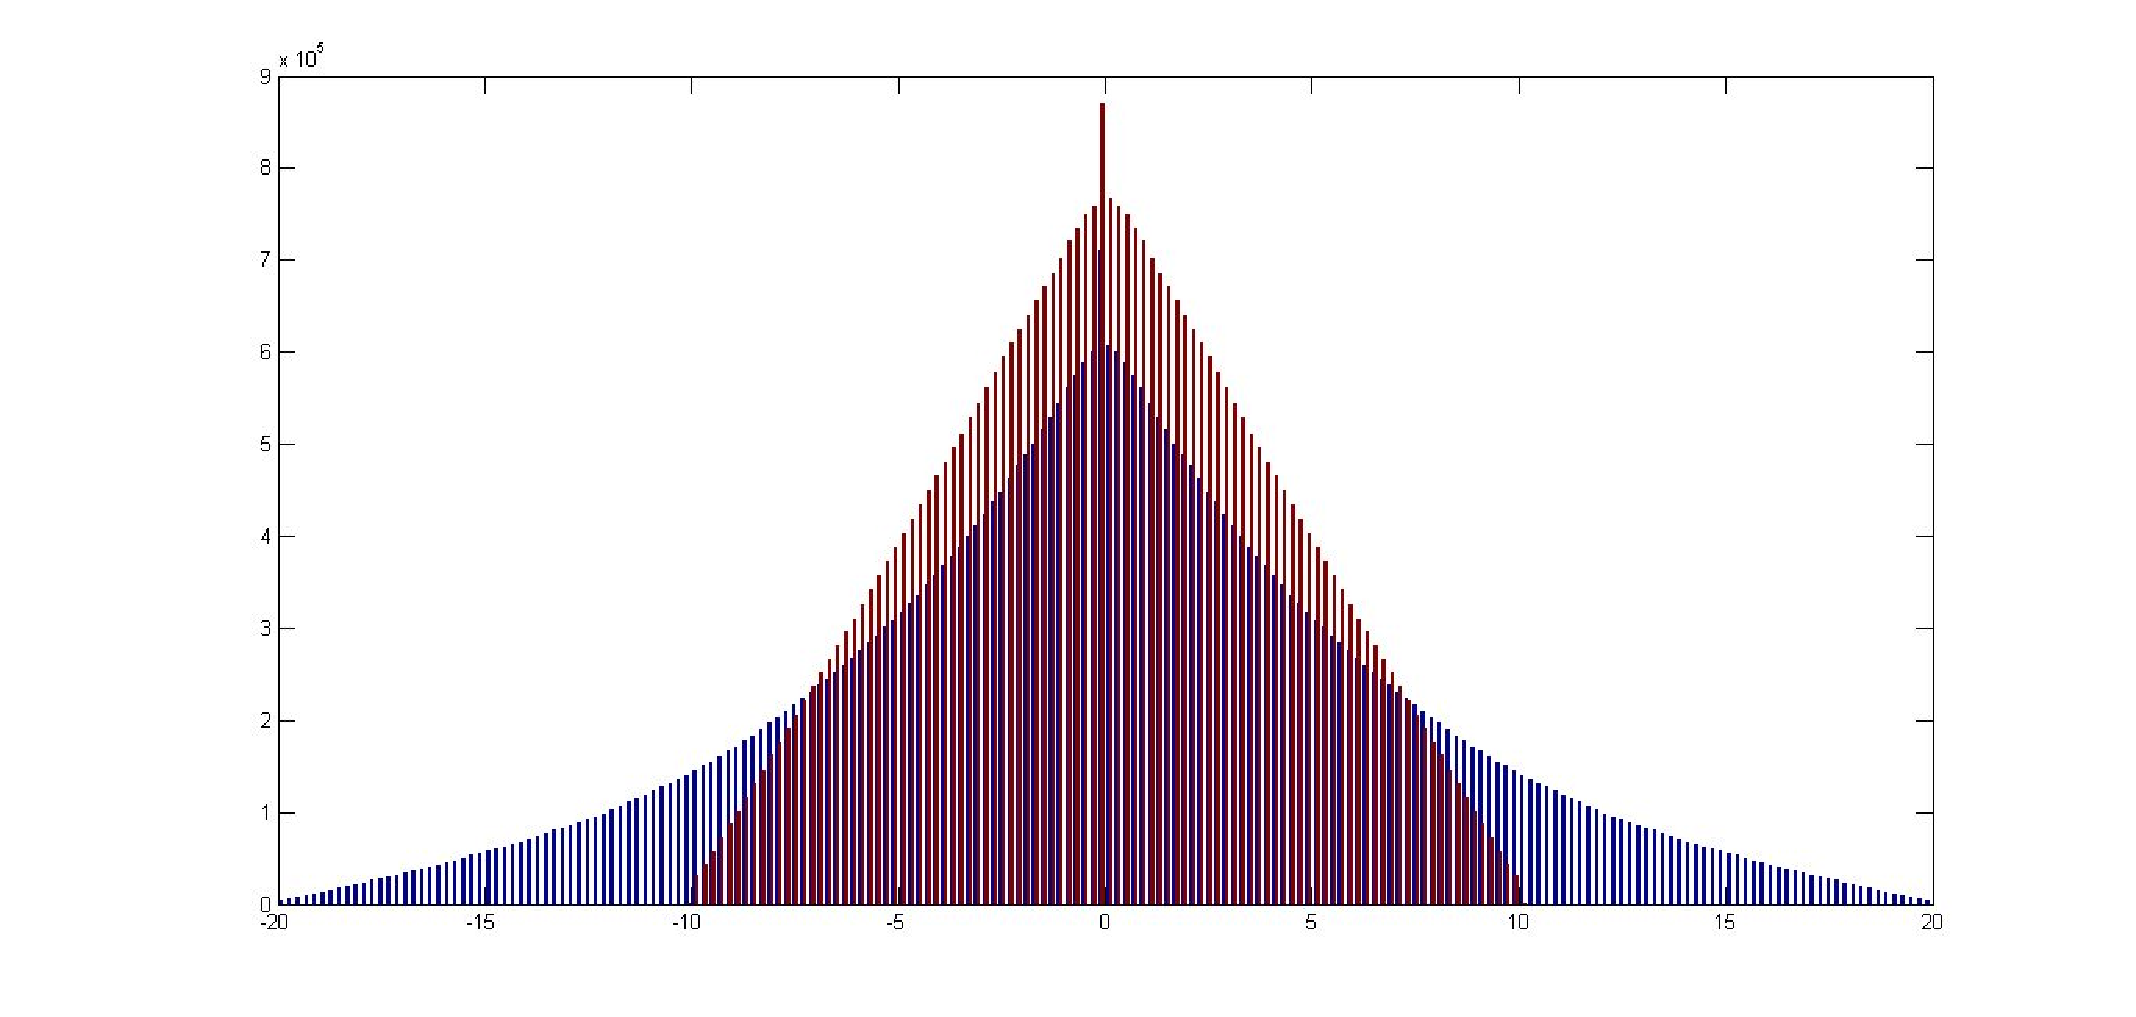
\includegraphics[width=\textwidth]{ri_n_10M_2__20_20__10_10_4_1D}
\caption{Rozkład prawdopodobieństwa punktów; 2 wymiary; generowanie z rozkładem normalnym; oddzielne histogramy dla obu wymiarów}
\label{bladzenie:reinicjacja2ds}
\end{figure}

\subsubsection*{Próbkowanie}
Ten rozkład charakteryzuje się spadkiem wartości prawdopodobieństwa wraz ze zbliżaniem się do ograniczenia. Punkty, które wypadłyby poza ograniczenia oraz ich potomkowie są przesuwane w kierunku środka przedziału.

\begin{figure}[H]
\centering
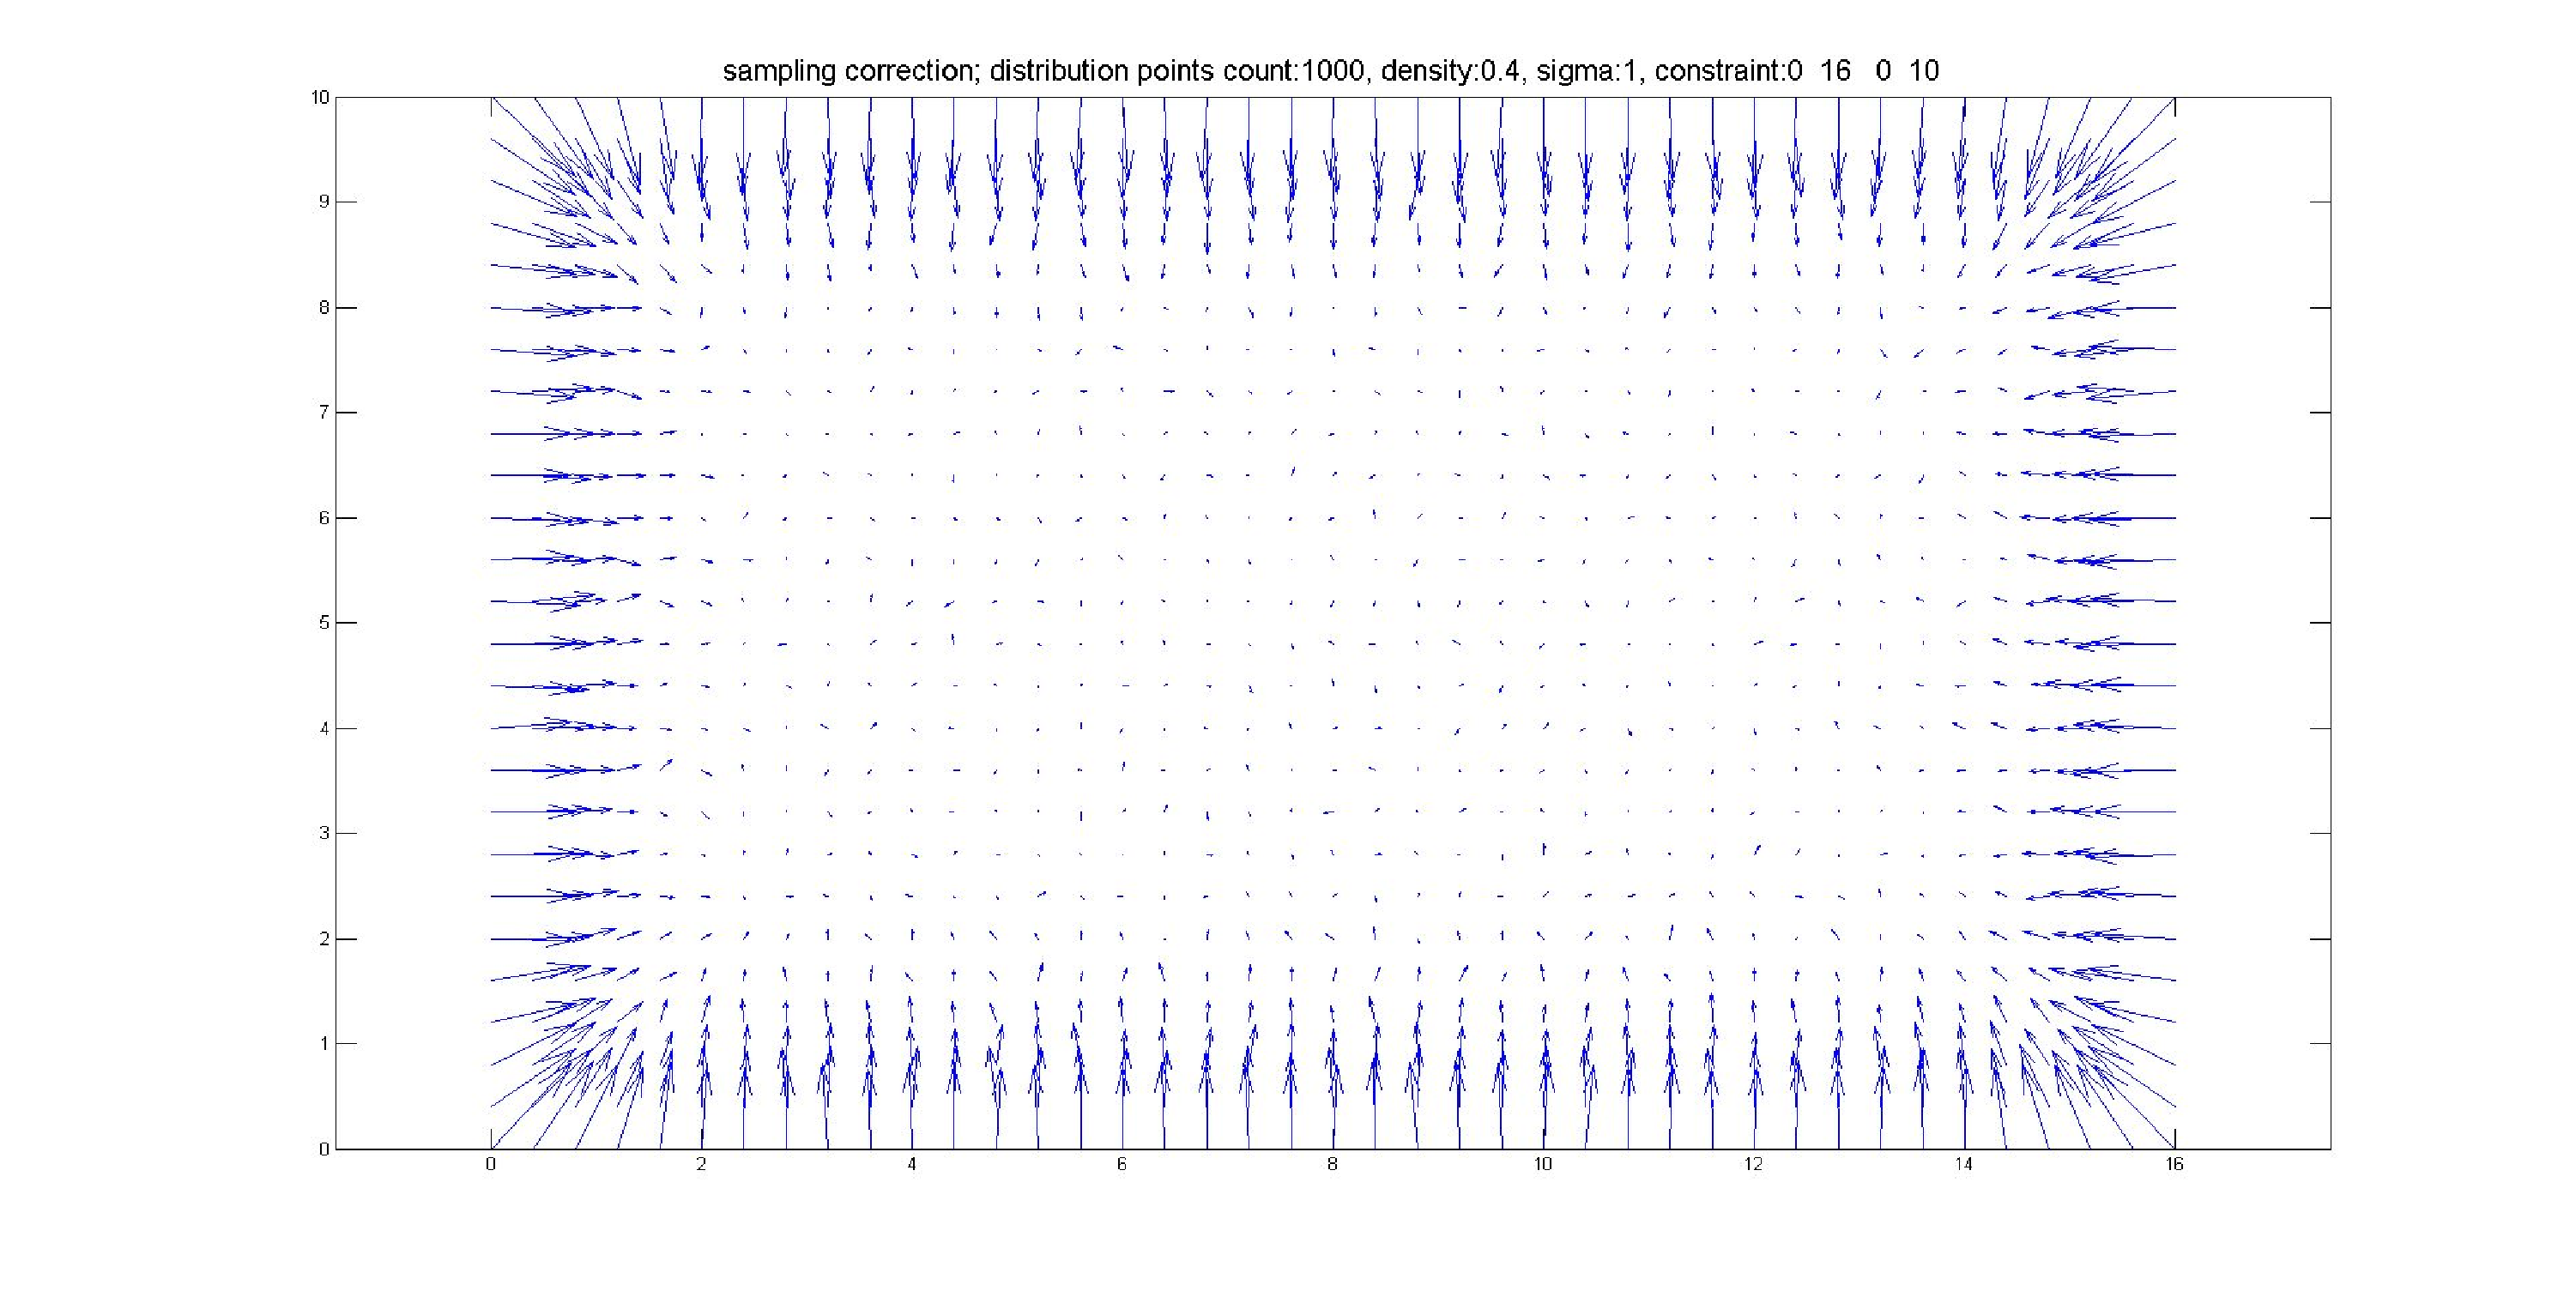
\includegraphics[width=\textwidth]{sampling2dprzesuniecie}
\caption{Wartość oczekiwana punktu}
\end{figure}

\begin{figure}[H]
\centering
\subfloat[Generowanie z rozkładem normalnym]{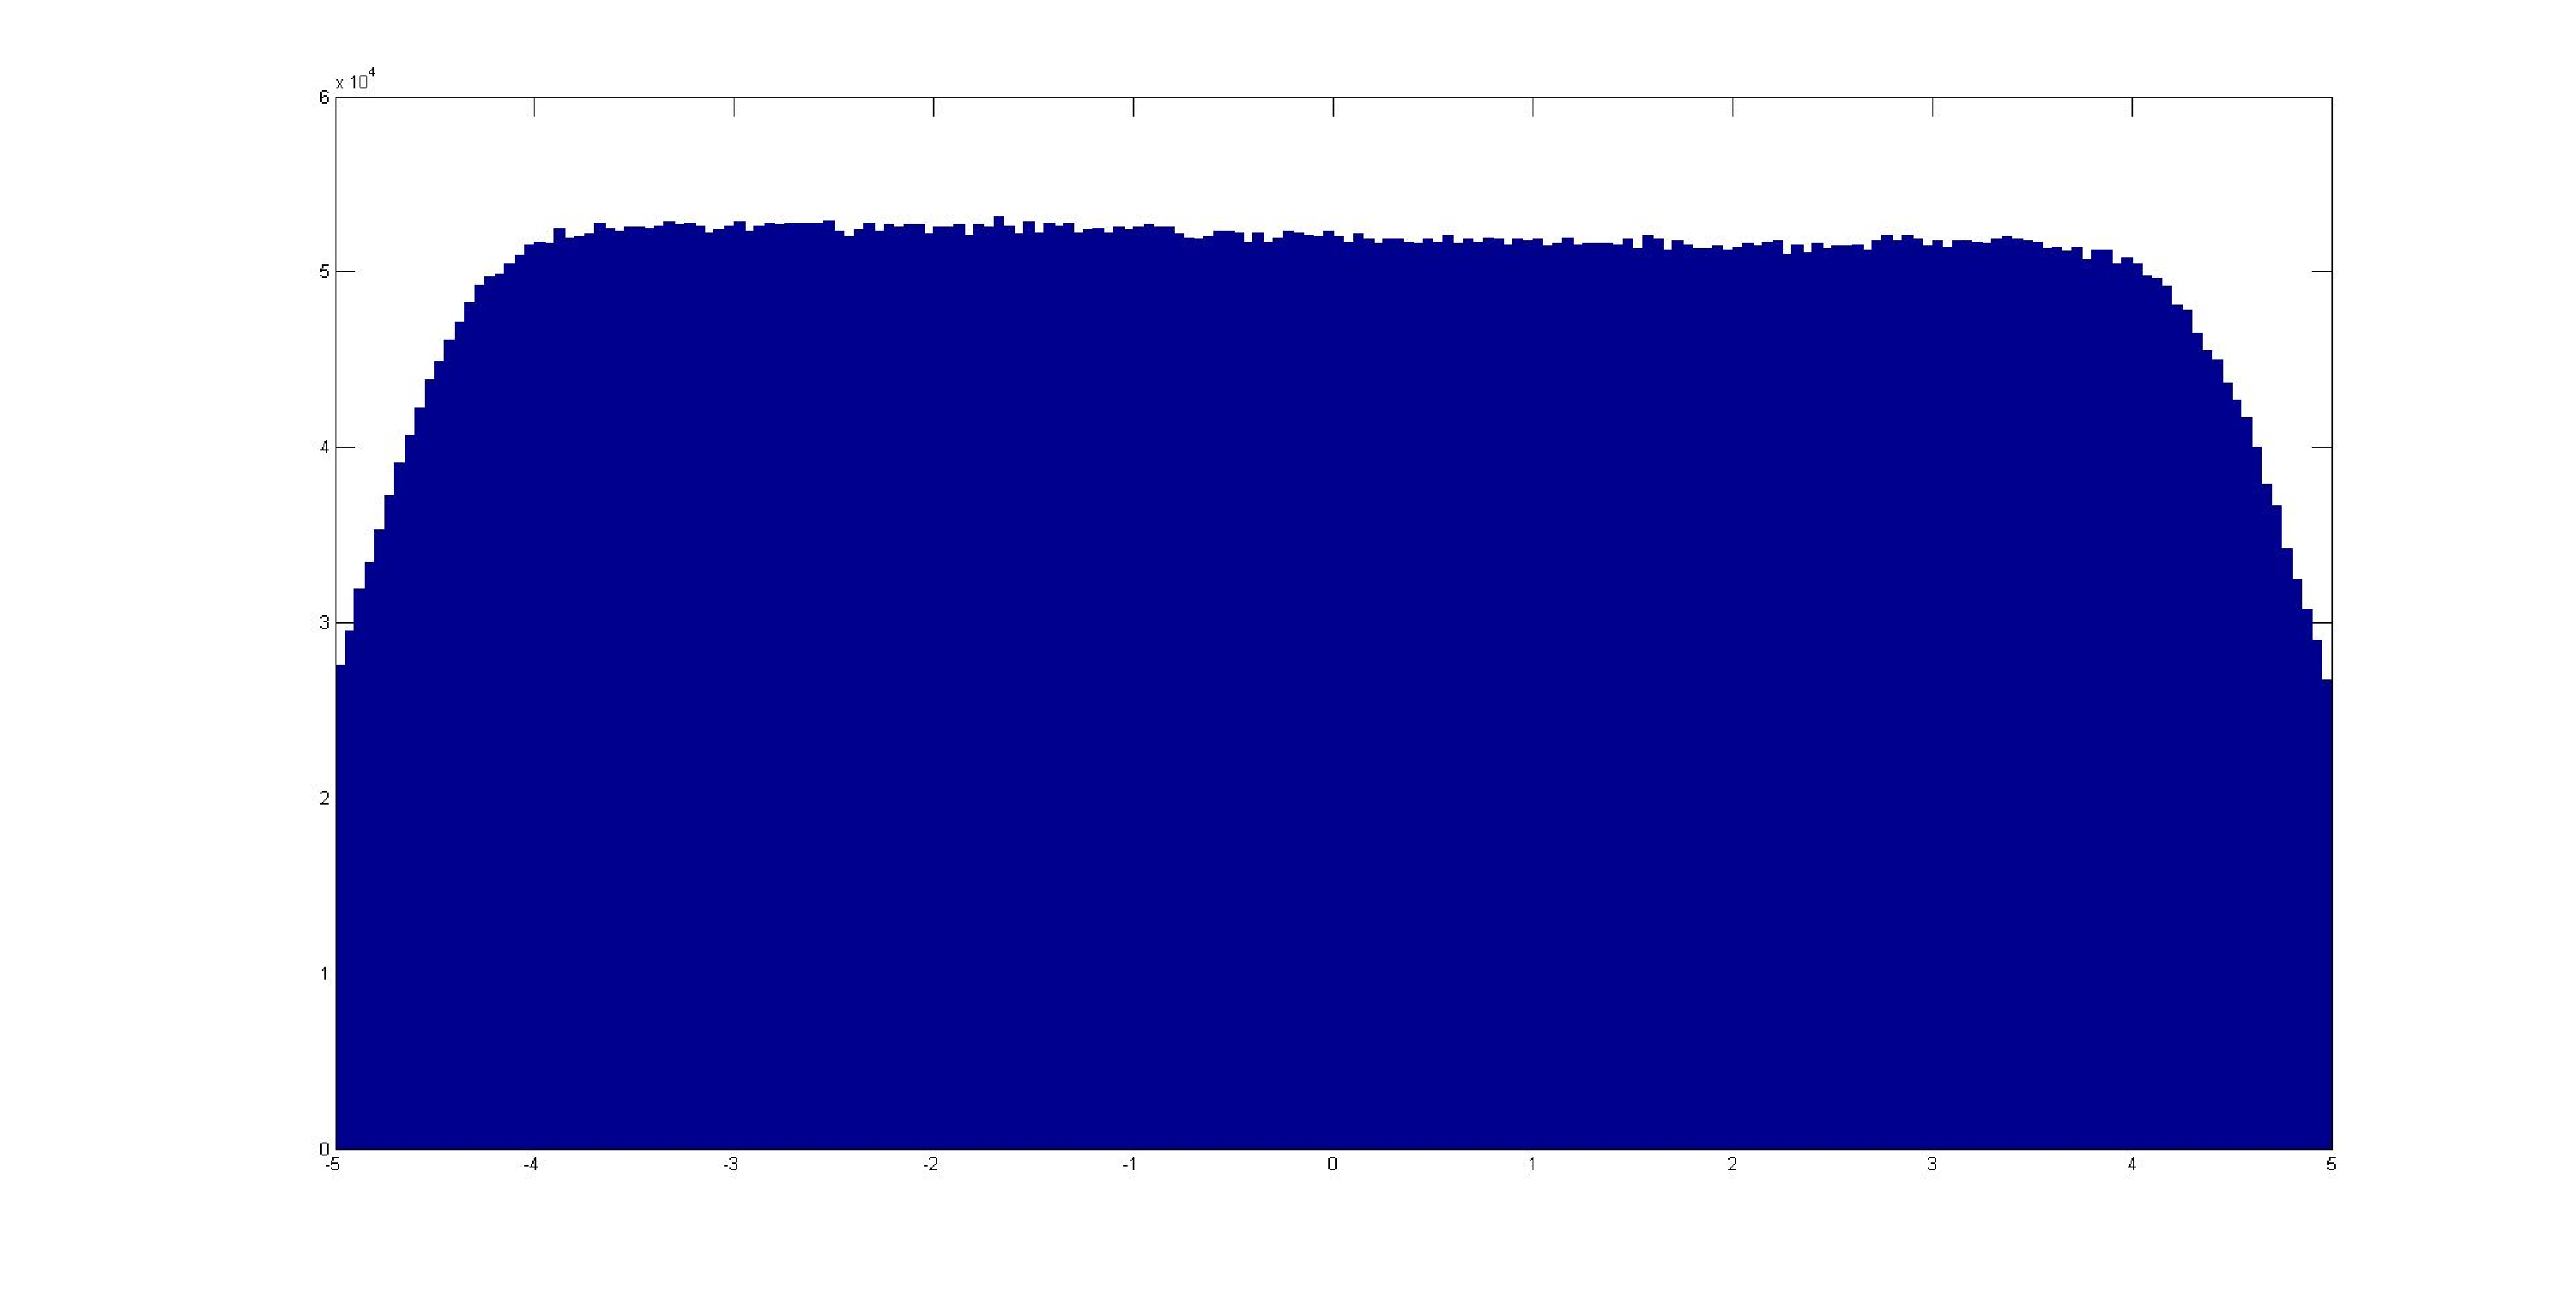
\includegraphics[width=0.45\textwidth]{s_n_10M_1__5_5}}
\quad
\subfloat[Generowanie z rozkładem jednostajnym]{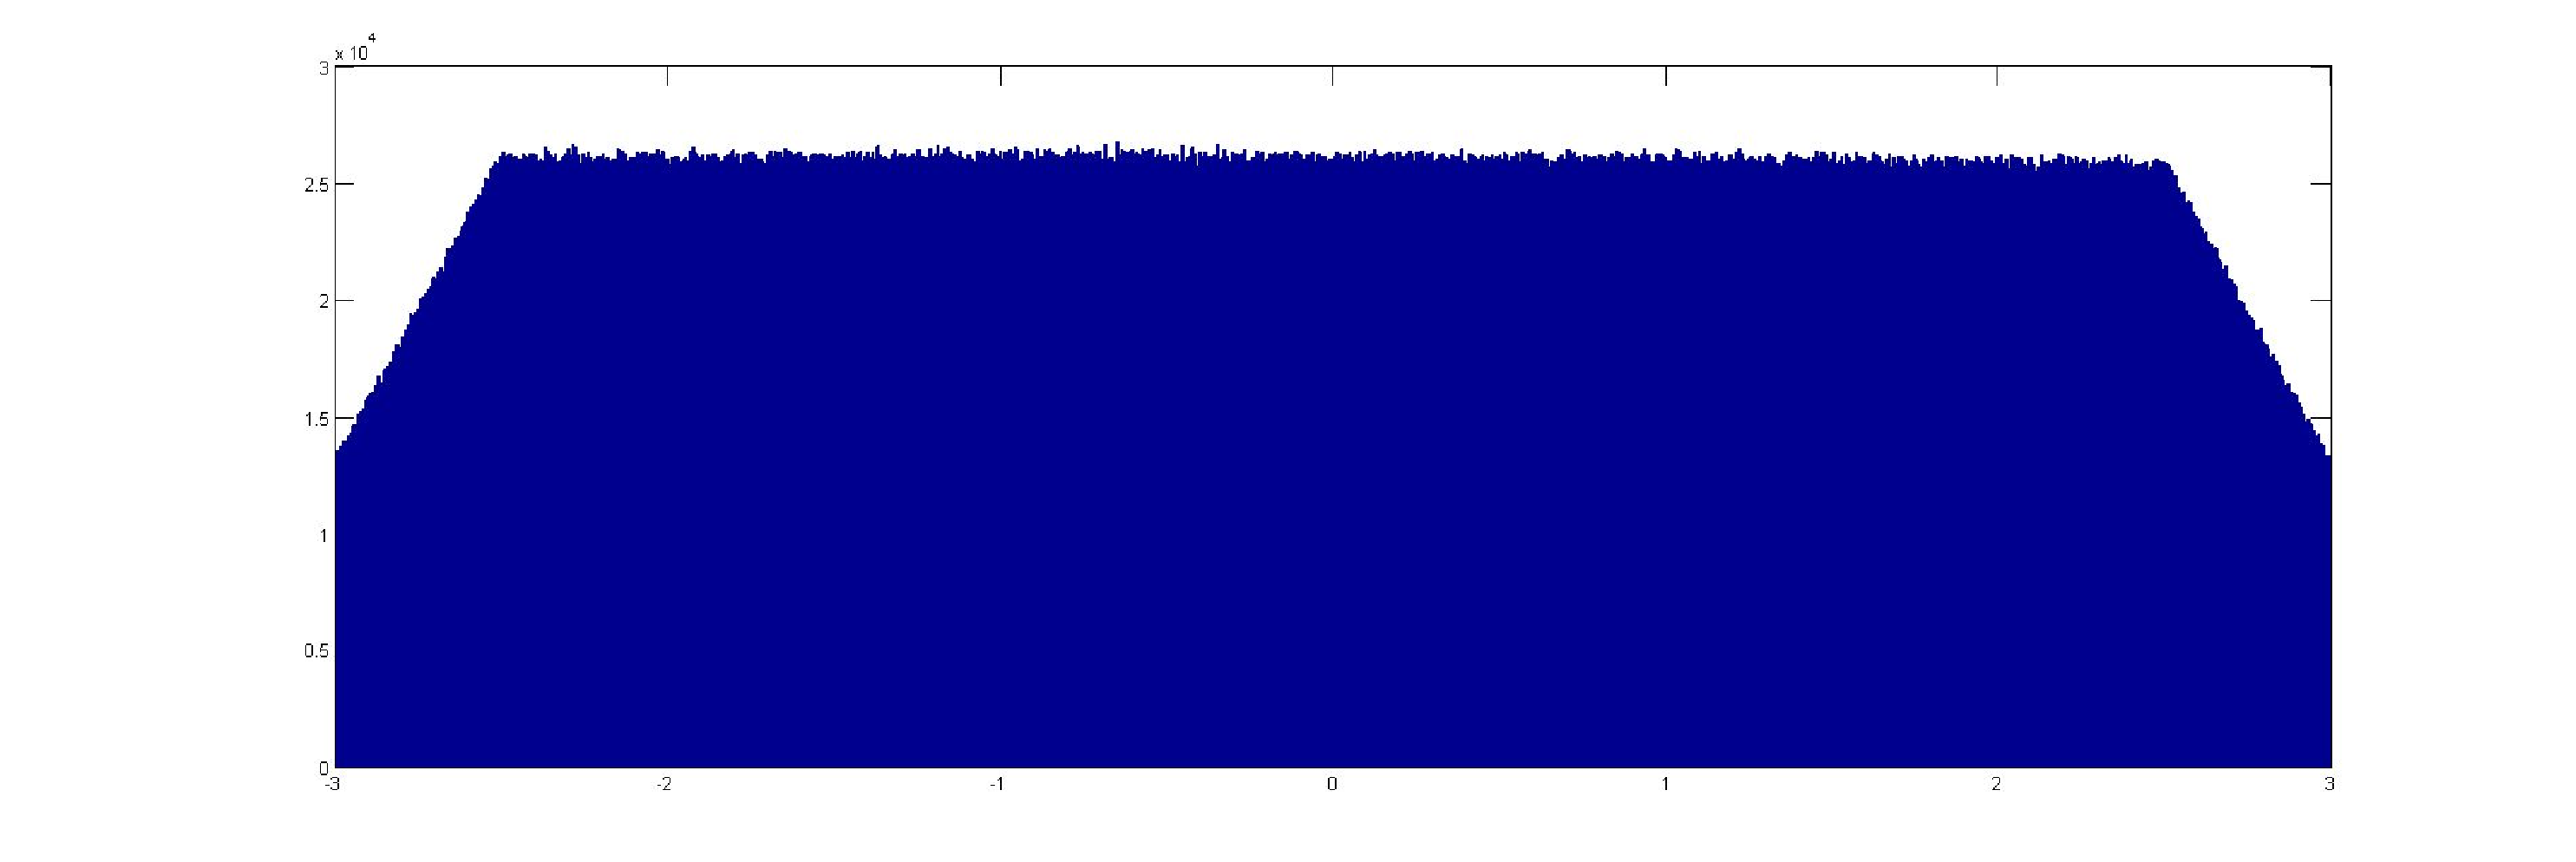
\includegraphics[width=0.45\textwidth]{s_j_20M_1__3_3}}
\caption{Rozkład prawdopodobieństwa punktów; 1 wymiar}
\end{figure}

\begin{figure}[H]
\centering
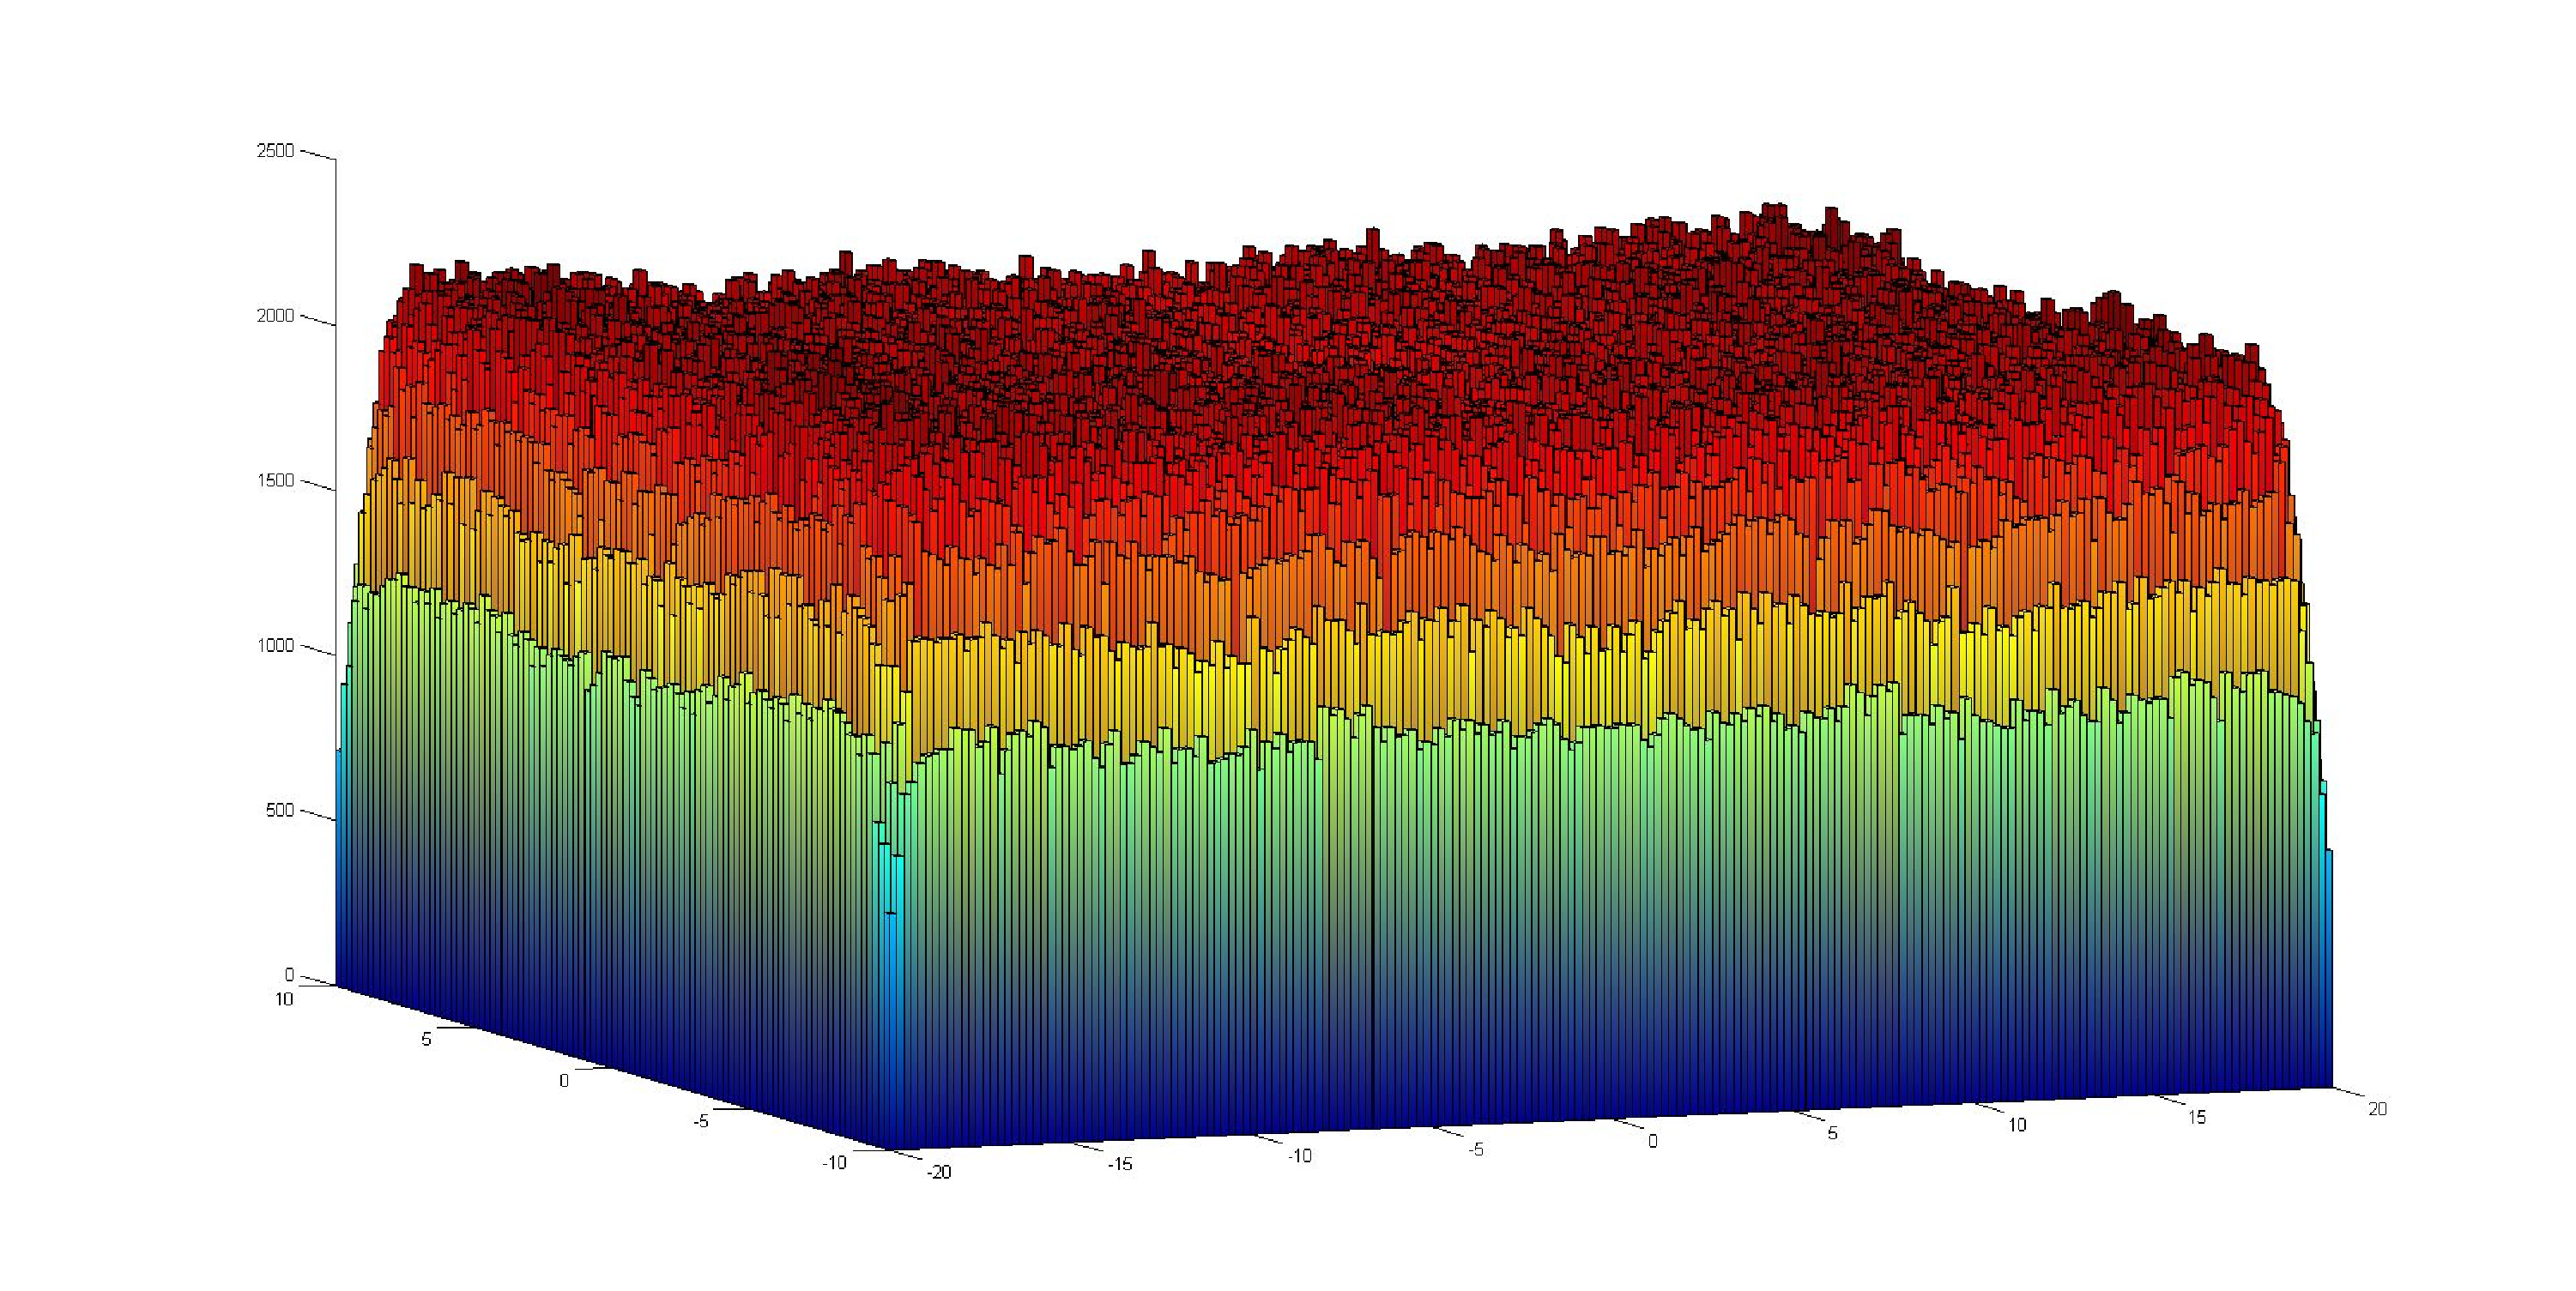
\includegraphics[width=\textwidth]{s_n_10M_2__20_20__10_10_4_2}
\caption{Rozkład prawdopodobieństwa punktów; 2 wymiary; generowanie z rozkładem normalnym}
\end{figure}

\subsubsection*{Zawijanie}
Wykres przesunięć wartości oczekiwanych jest bardzo nieczytelny. Jest to implikacji dużych przesunięć punktów - te, które znajdą się poza ograniczeniem, wędrują na drugą stronę wykresu.

Uzasadniając wykresy histogramów warto wyobrazić sobie, że symulacja przeprowadzana jest bez ograniczeń, a następnie wykres z wynikami przecinany jest w równych odstępach wzdłuż każdej osi. Na koniec tak pocięte części łączone są w jeden wykres. Takie zachowanie symuluje zawijanie. W związku z tym nie dziwi fakt, że histogramy przedstawiają rozkład jednostajny z szumem.

\begin{figure}[H]
\centering
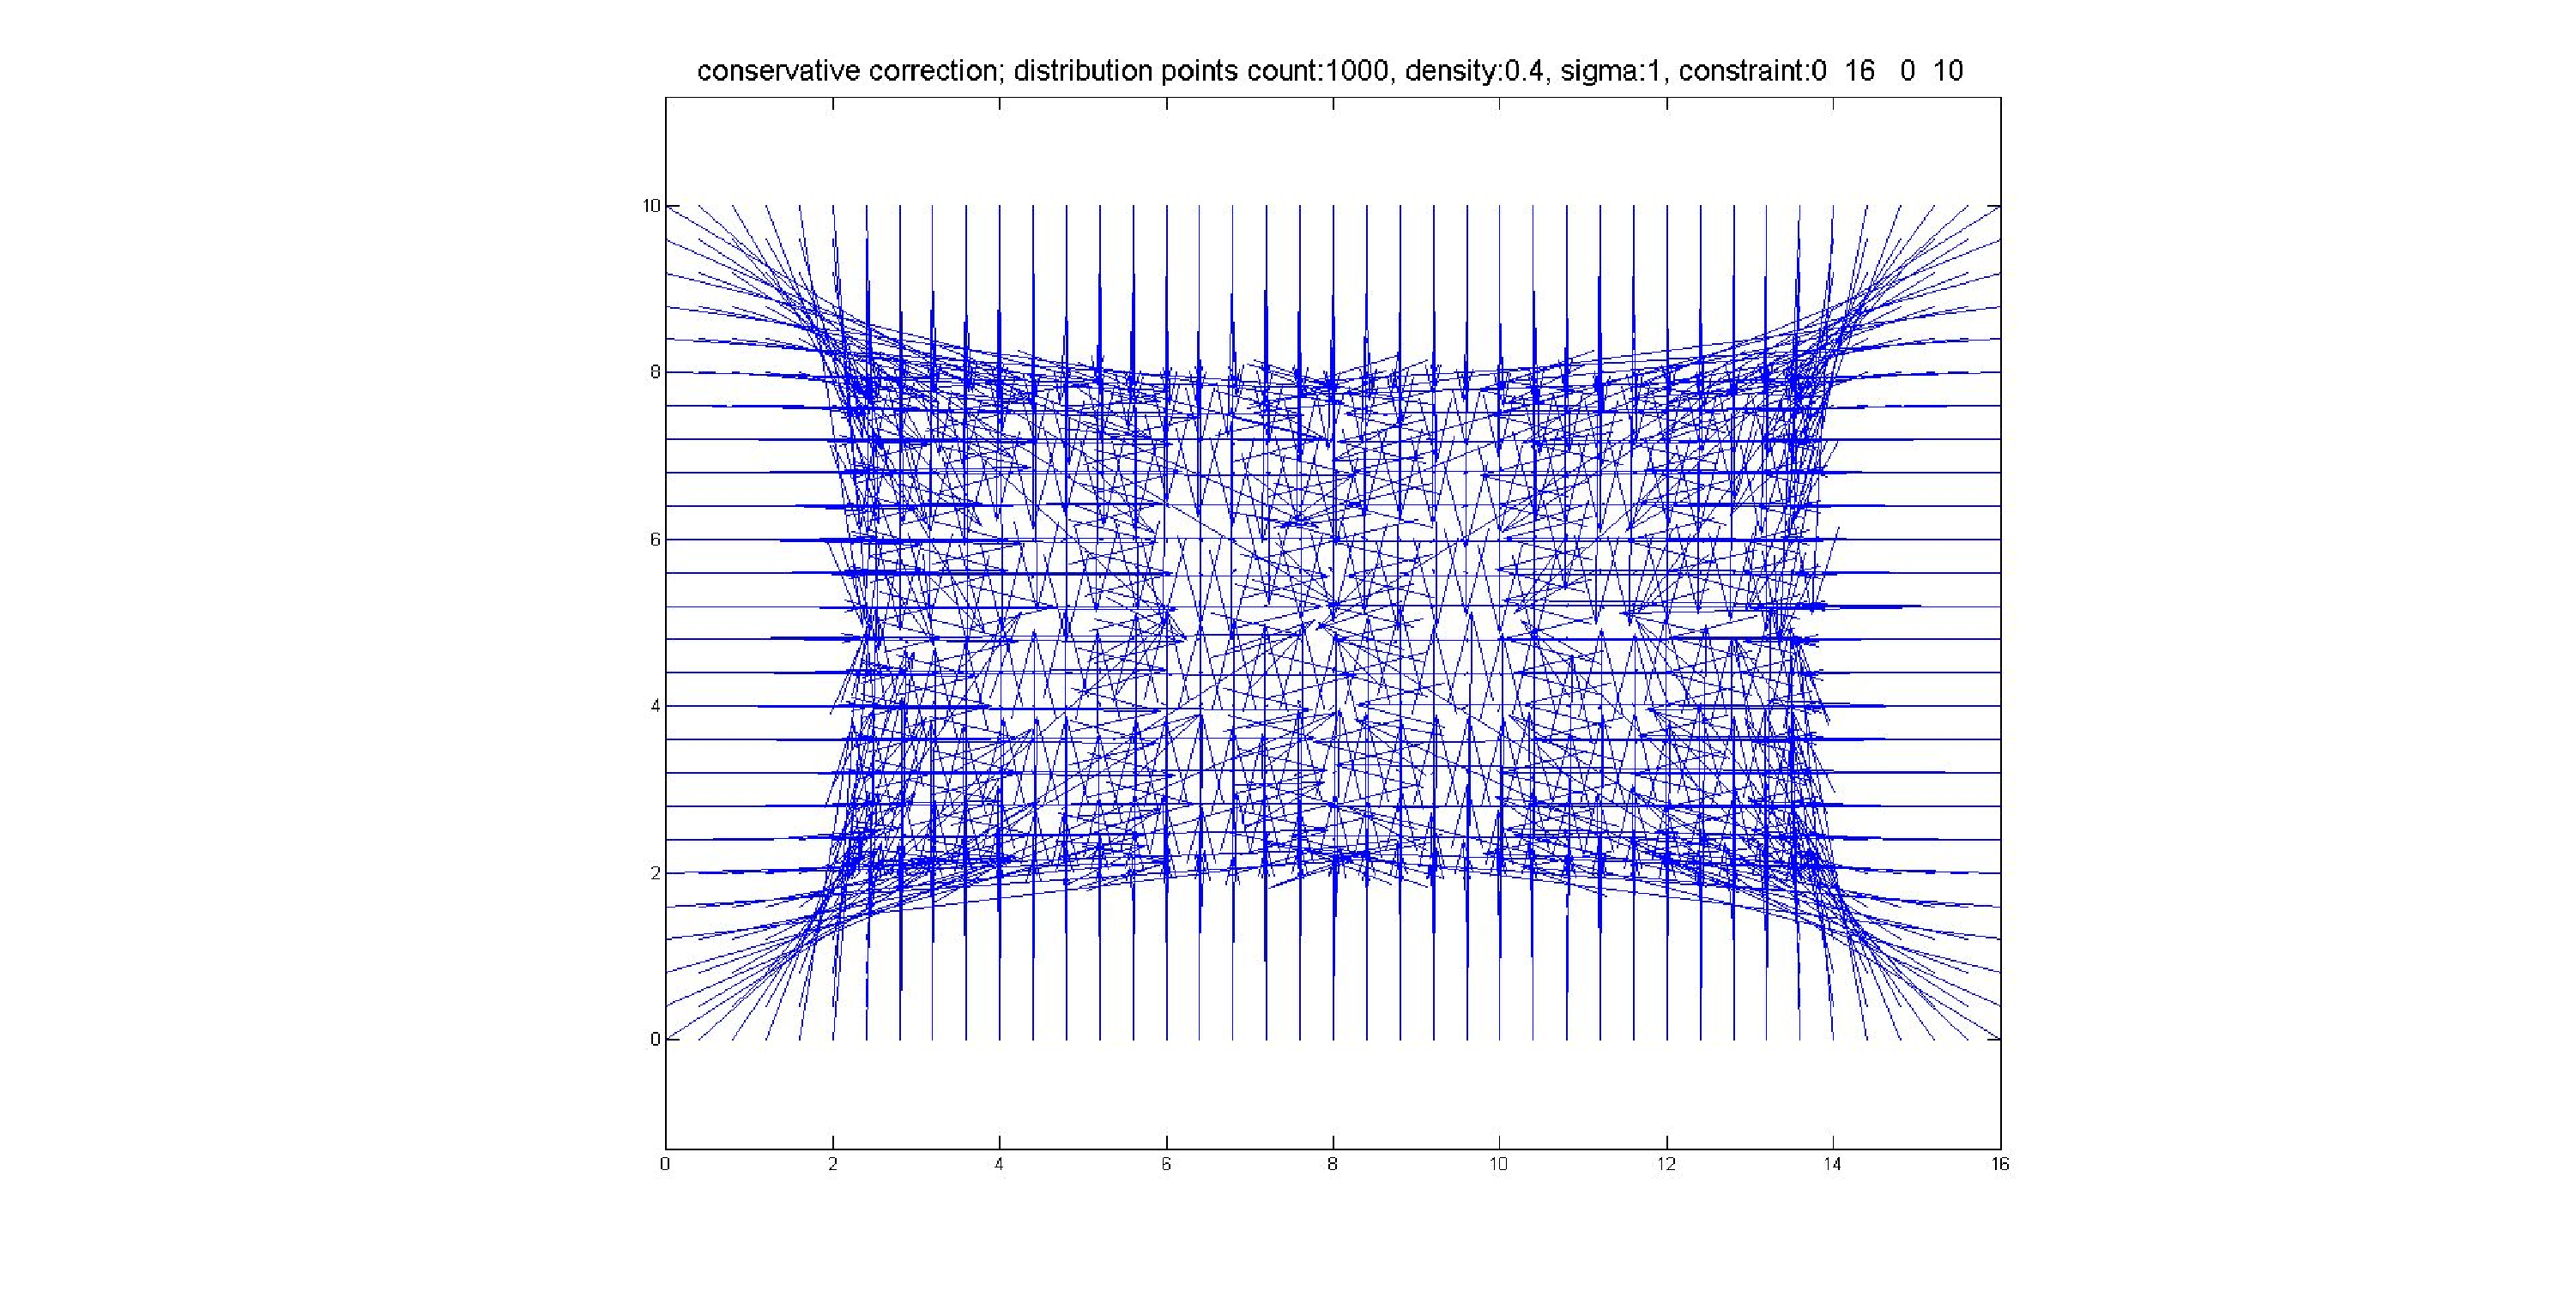
\includegraphics[width=\textwidth]{wrapping2dprzesuniecie}
\caption{Wartość oczekiwana punktu}
\end{figure}

\begin{figure}[H]
\centering
\subfloat[1 wymiar; generowanie z rozkładem normalnym]{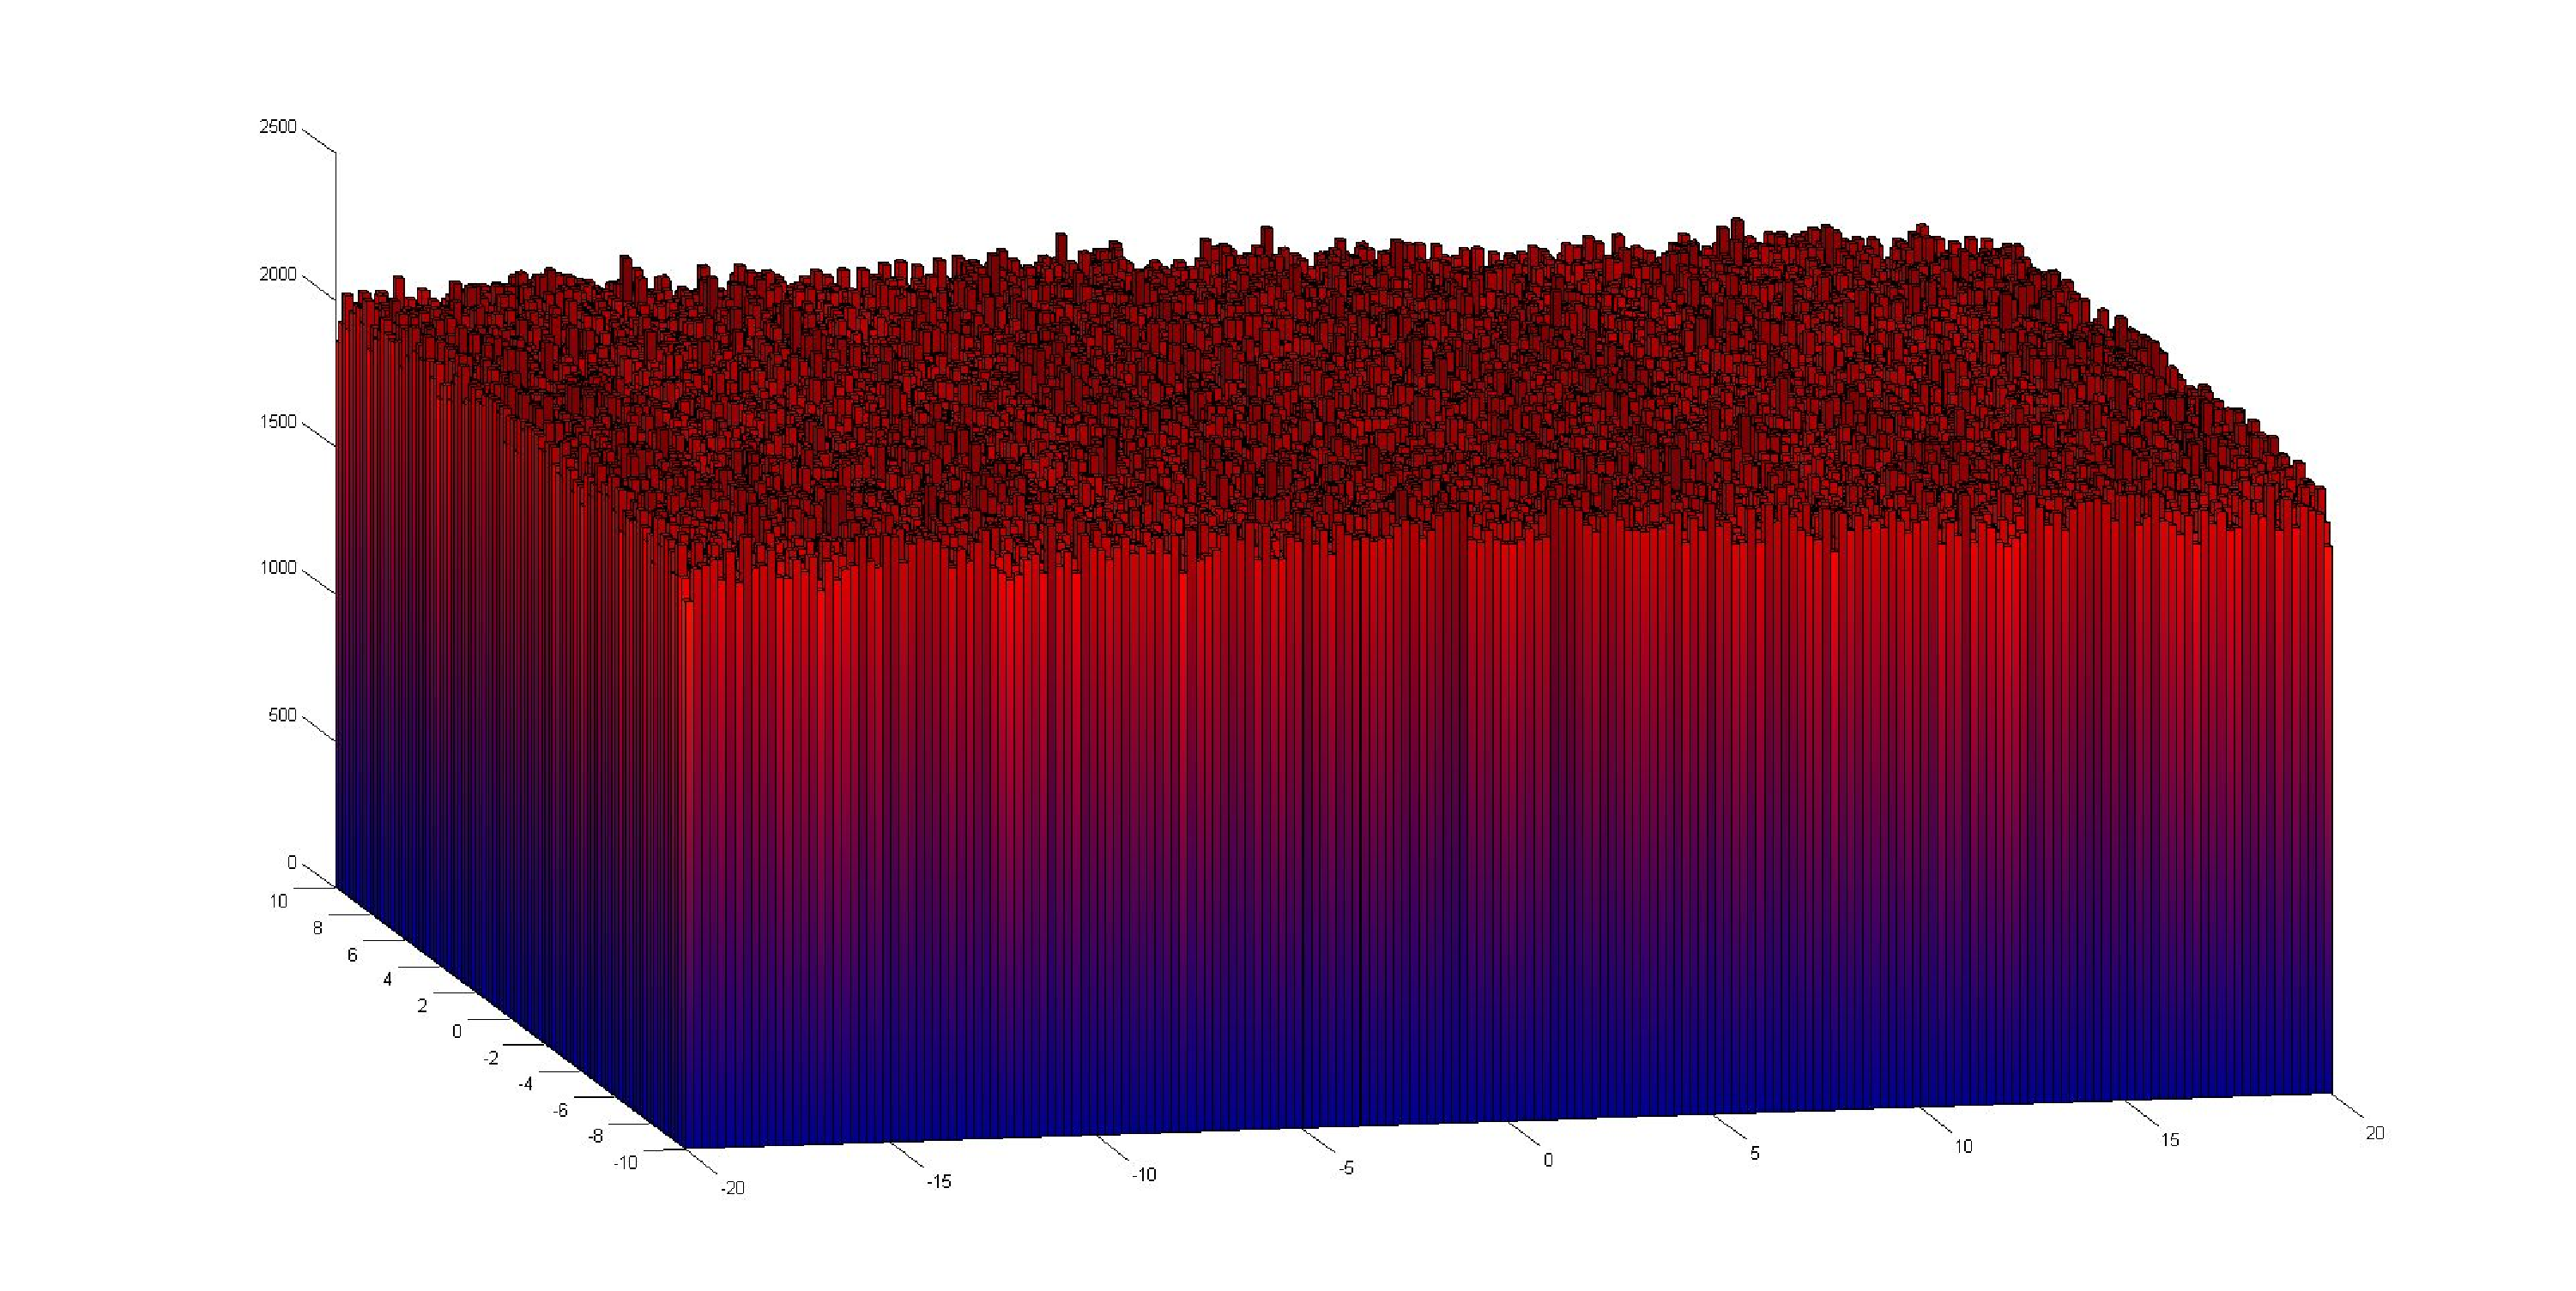
\includegraphics[width=0.45\textwidth]{w_n_10M_2__20_20__10_10_4_2}}
\quad
\subfloat[2 wymiary; generowanie z rozkładem jednostajnym]{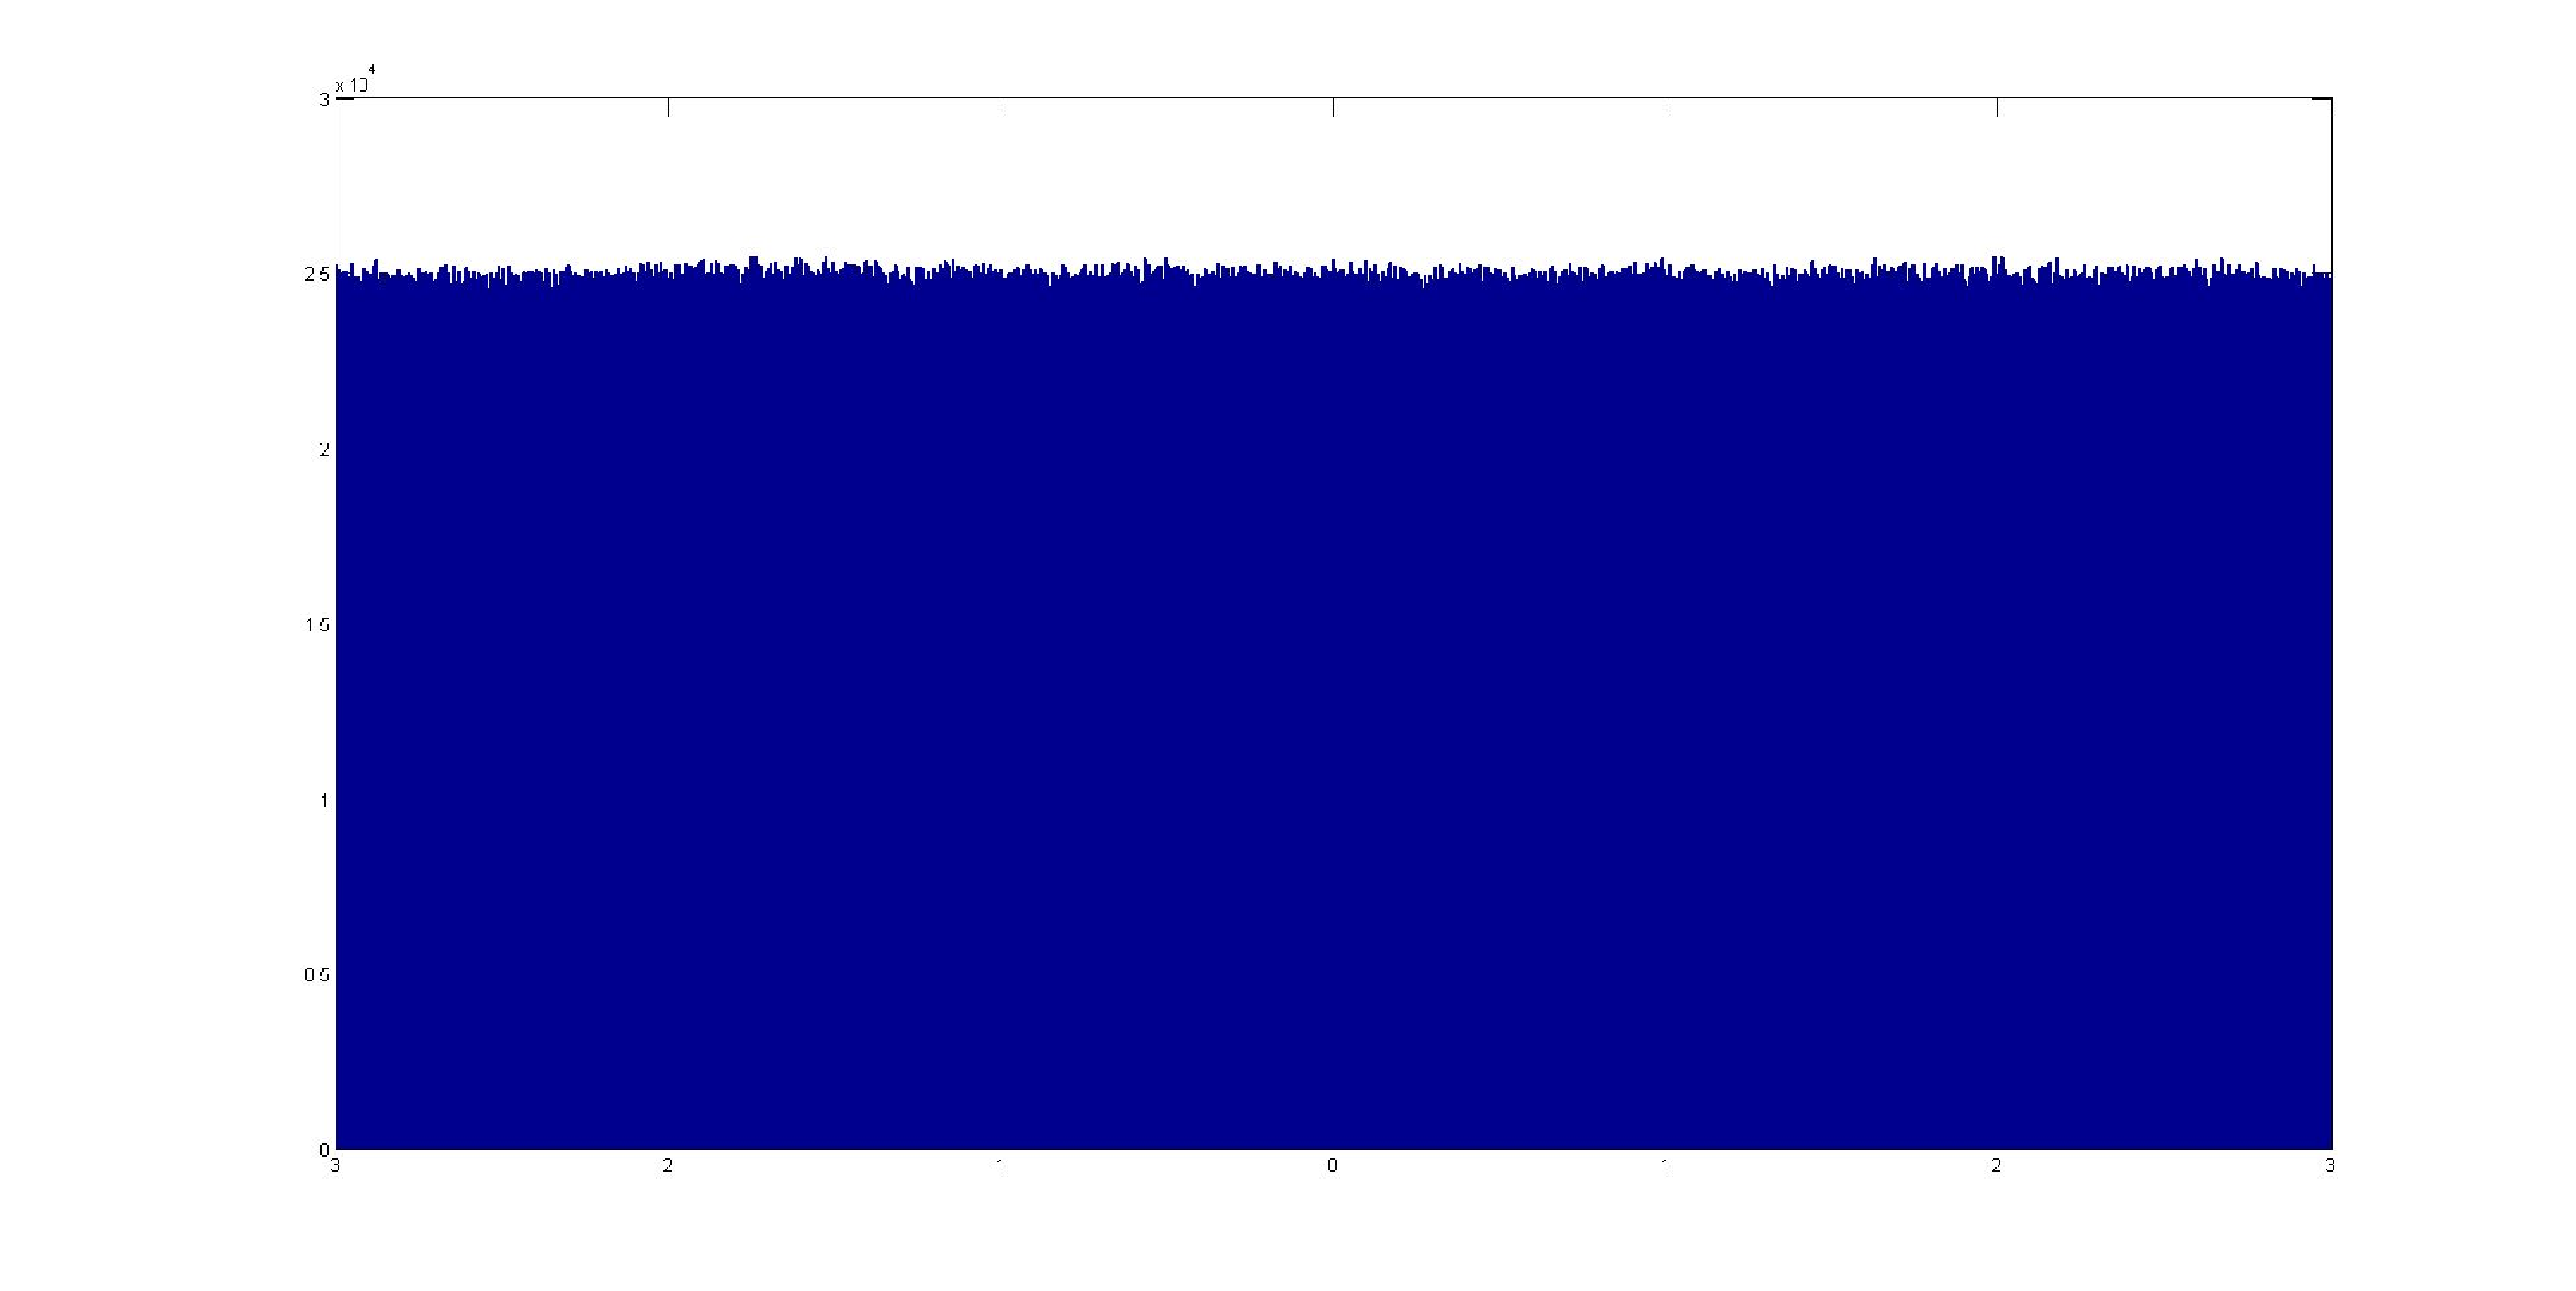
\includegraphics[width=0.45\textwidth]{w_j_20M_1__3_3}}
\caption{Rozkład prawdopodobieństwa punktów;}
\end{figure}

\subsubsection*{Odbicie}
Podobnie jak zawijanie, odbicie zwraca histogram rozkładu normalnego z szumem. W~tej sytuacji nieco trudniej o analogię, lecz po chwili zastanowienia nie dziwi kształt poniższych wykresów.

Od zawijania różni się natomiast wykres wartości oczekiwanych, ponieważ w odbiciu nie ma znaczących przesunięć punktów.

\begin{figure}[H]
\centering
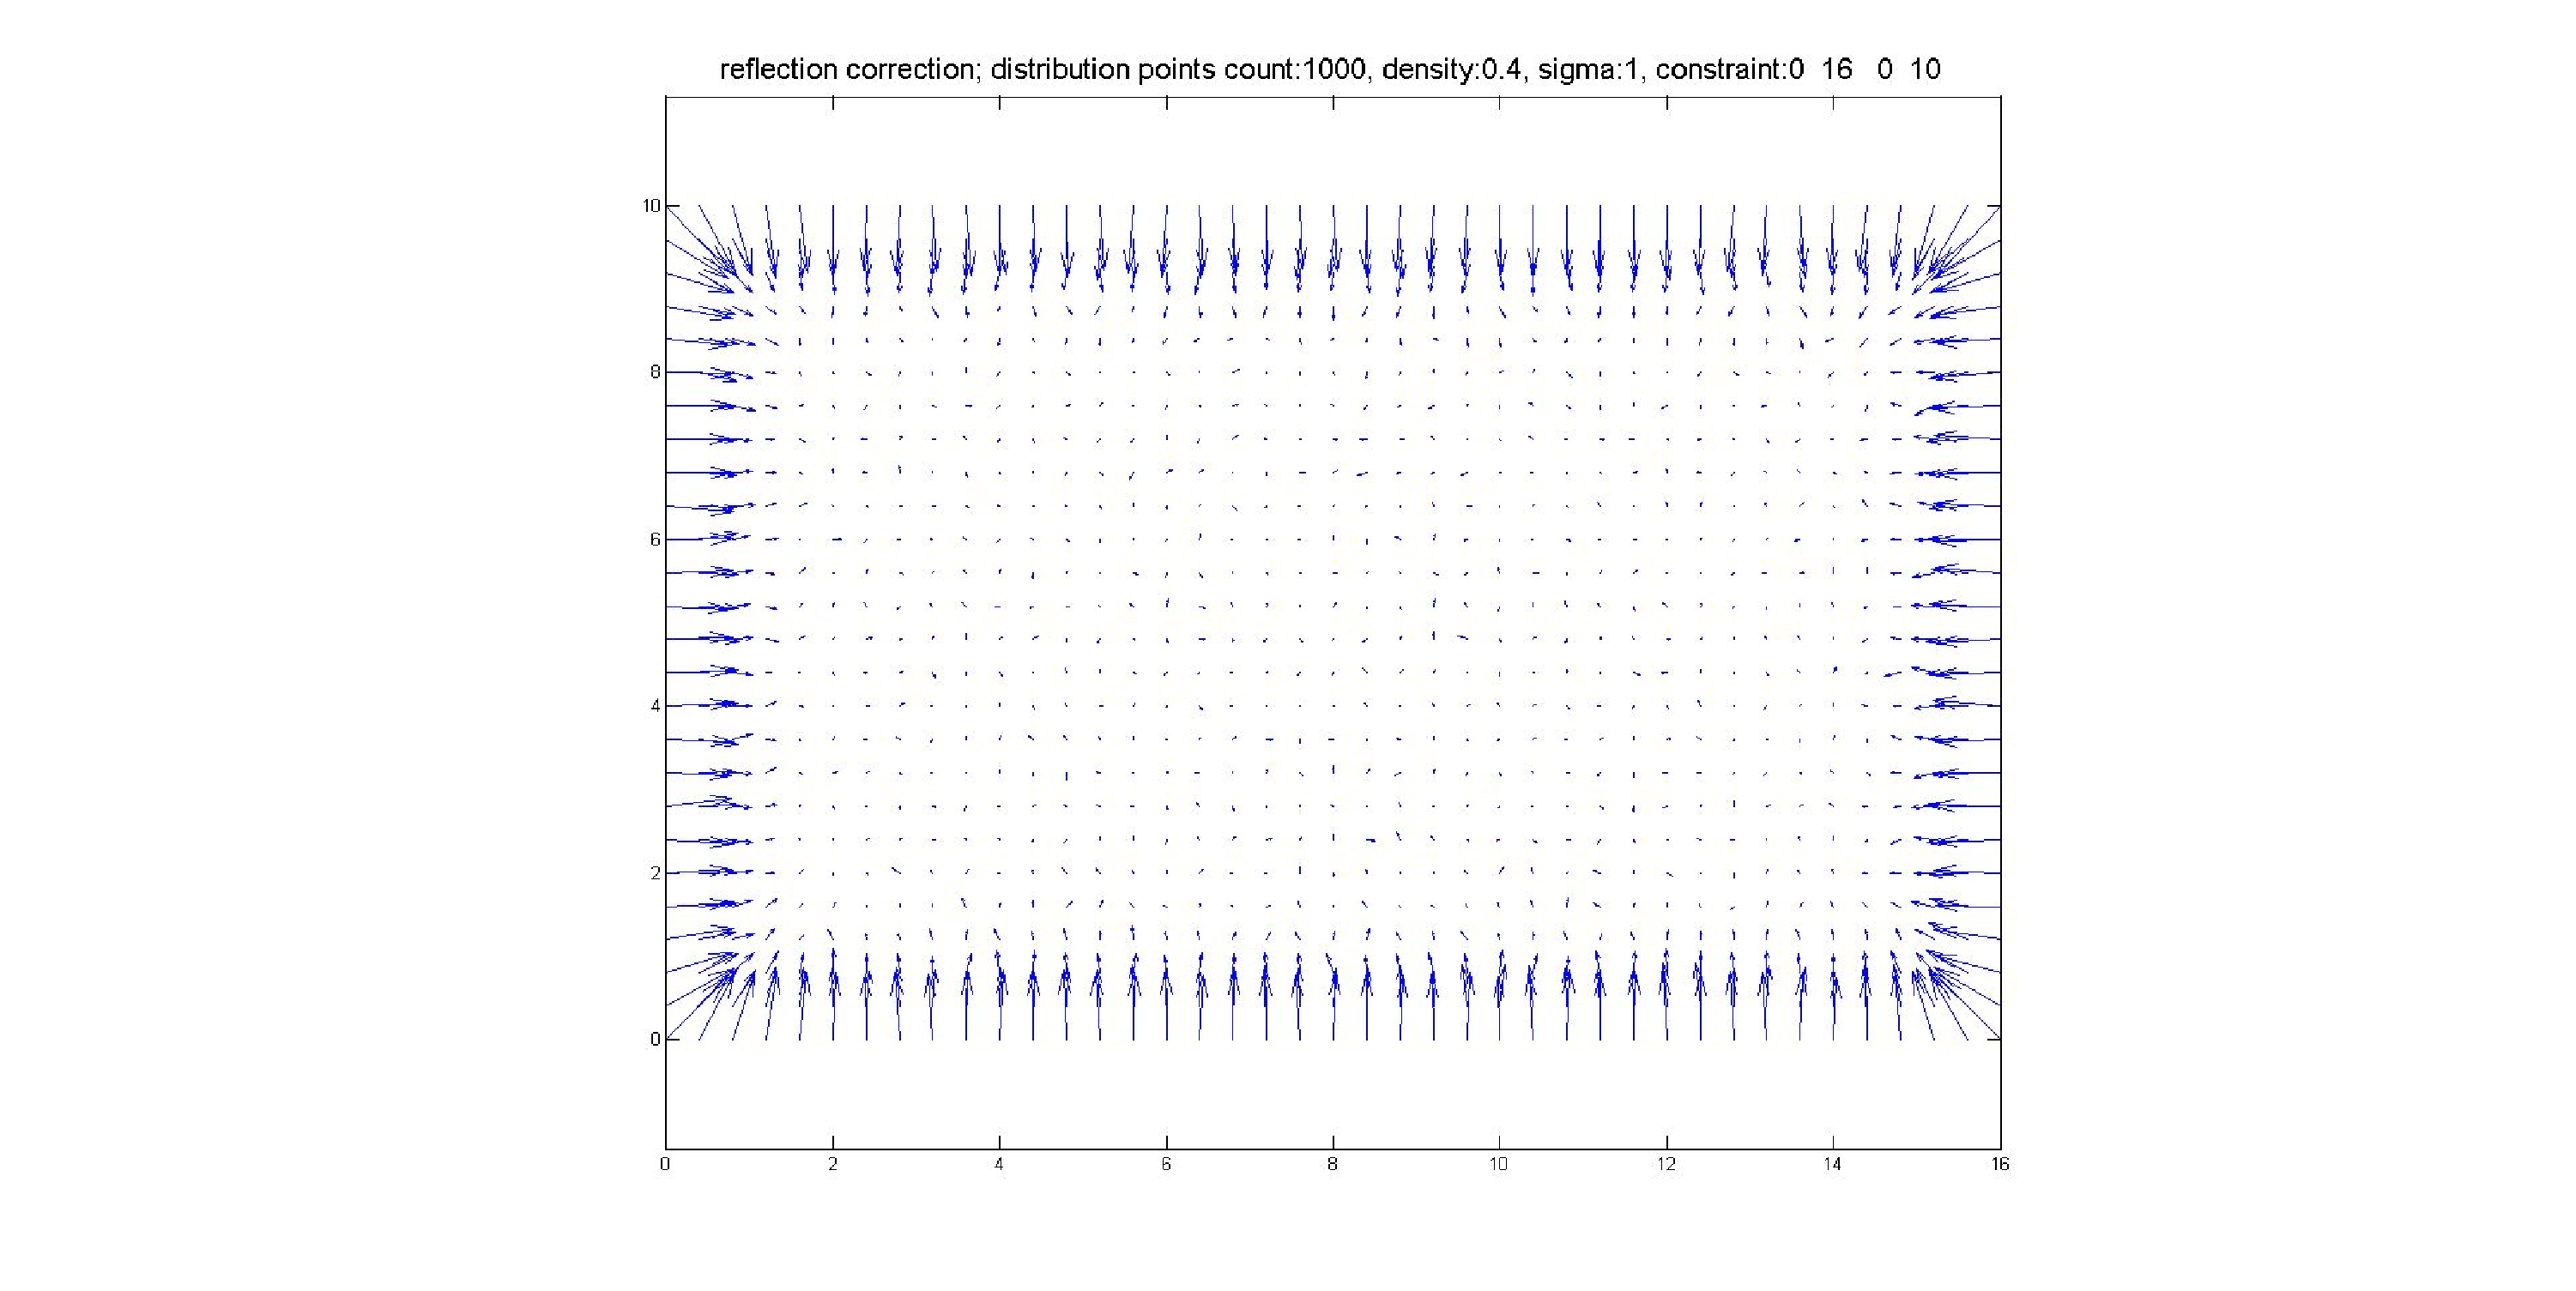
\includegraphics[width=\textwidth]{reflection2dprzesuniecie}
\caption{Wartość oczekiwana punktu}
\end{figure}

\begin{figure}[H]
\centering
\subfloat[1 wymiar; generowanie z rozkładem normalnym]{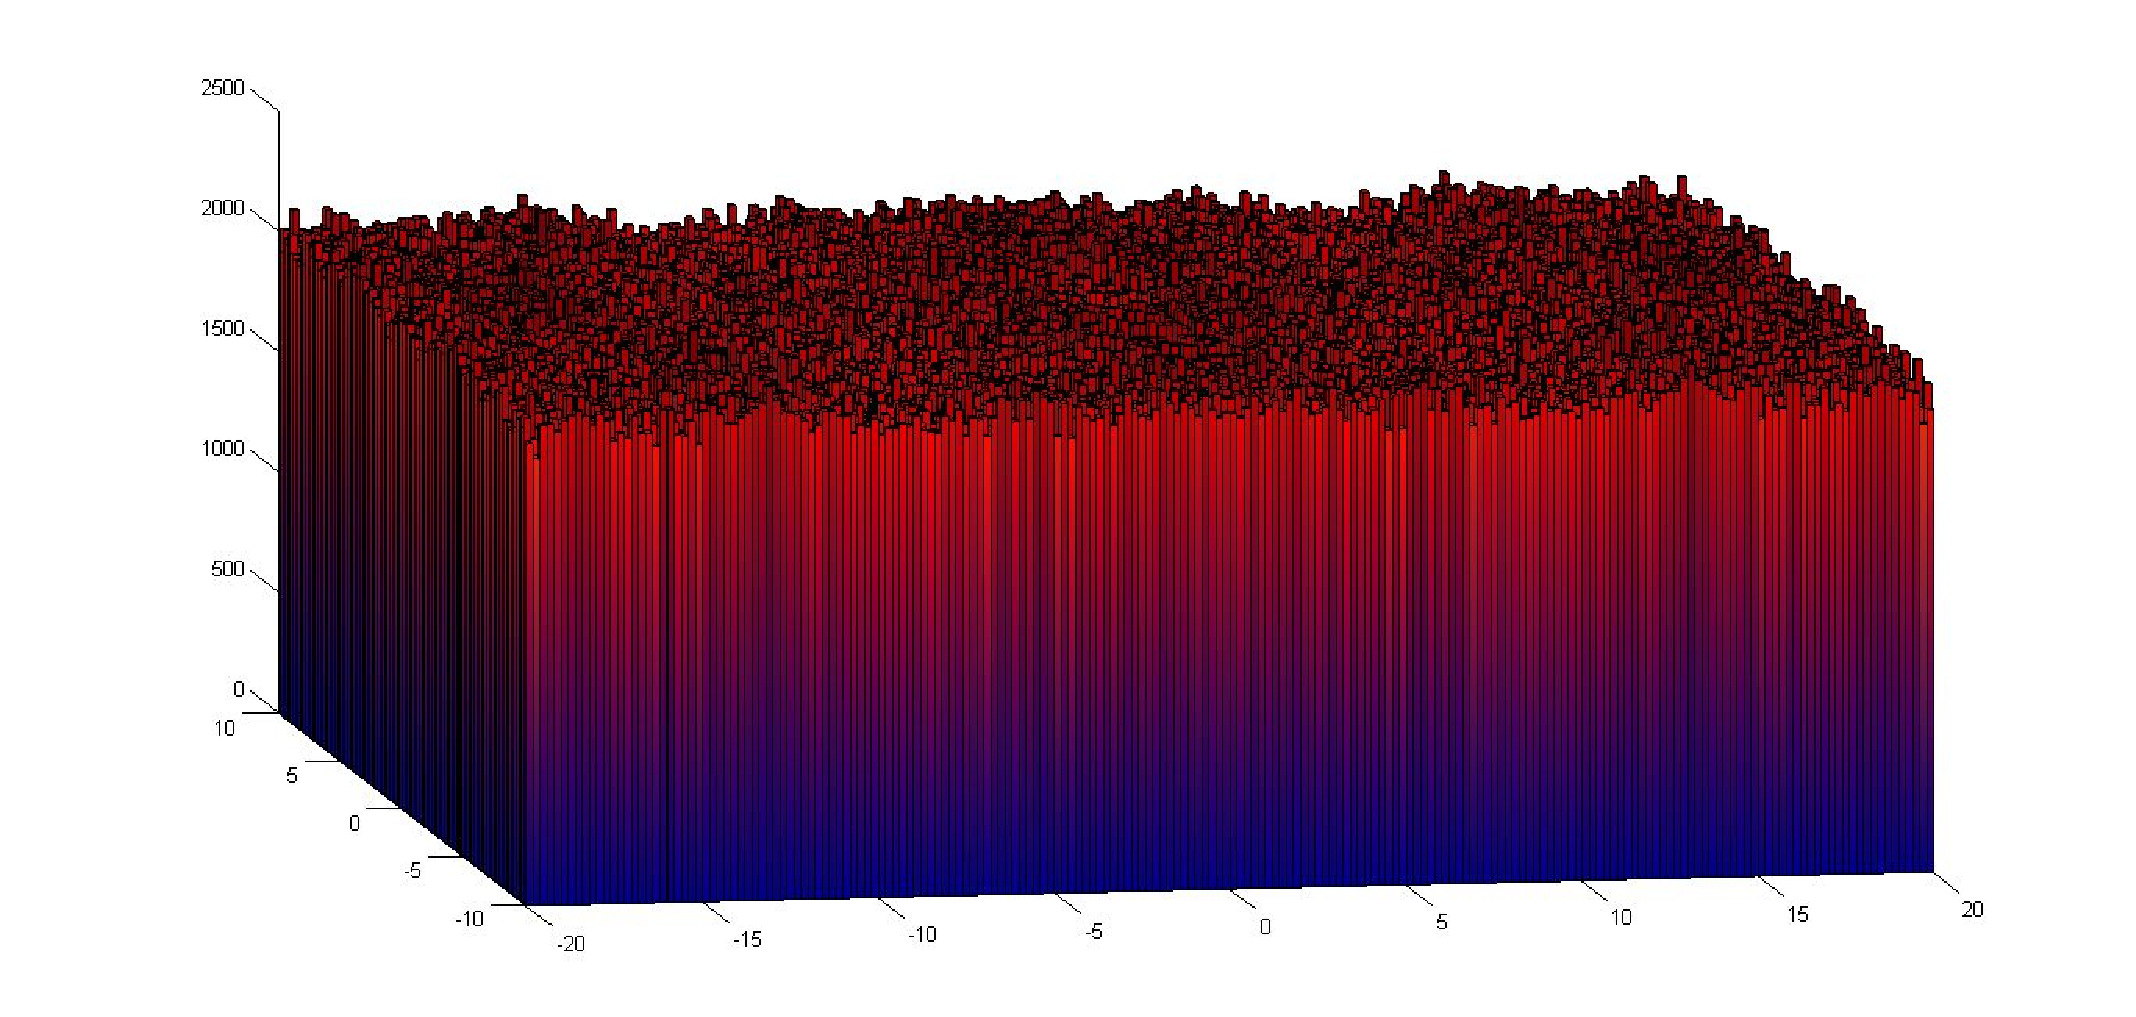
\includegraphics[width=0.45\textwidth]{rf_n_10M_2__20_20__10_10_4_2}}
\quad
\subfloat[2 wymiary; generowanie z rozkładem jednostajnym]{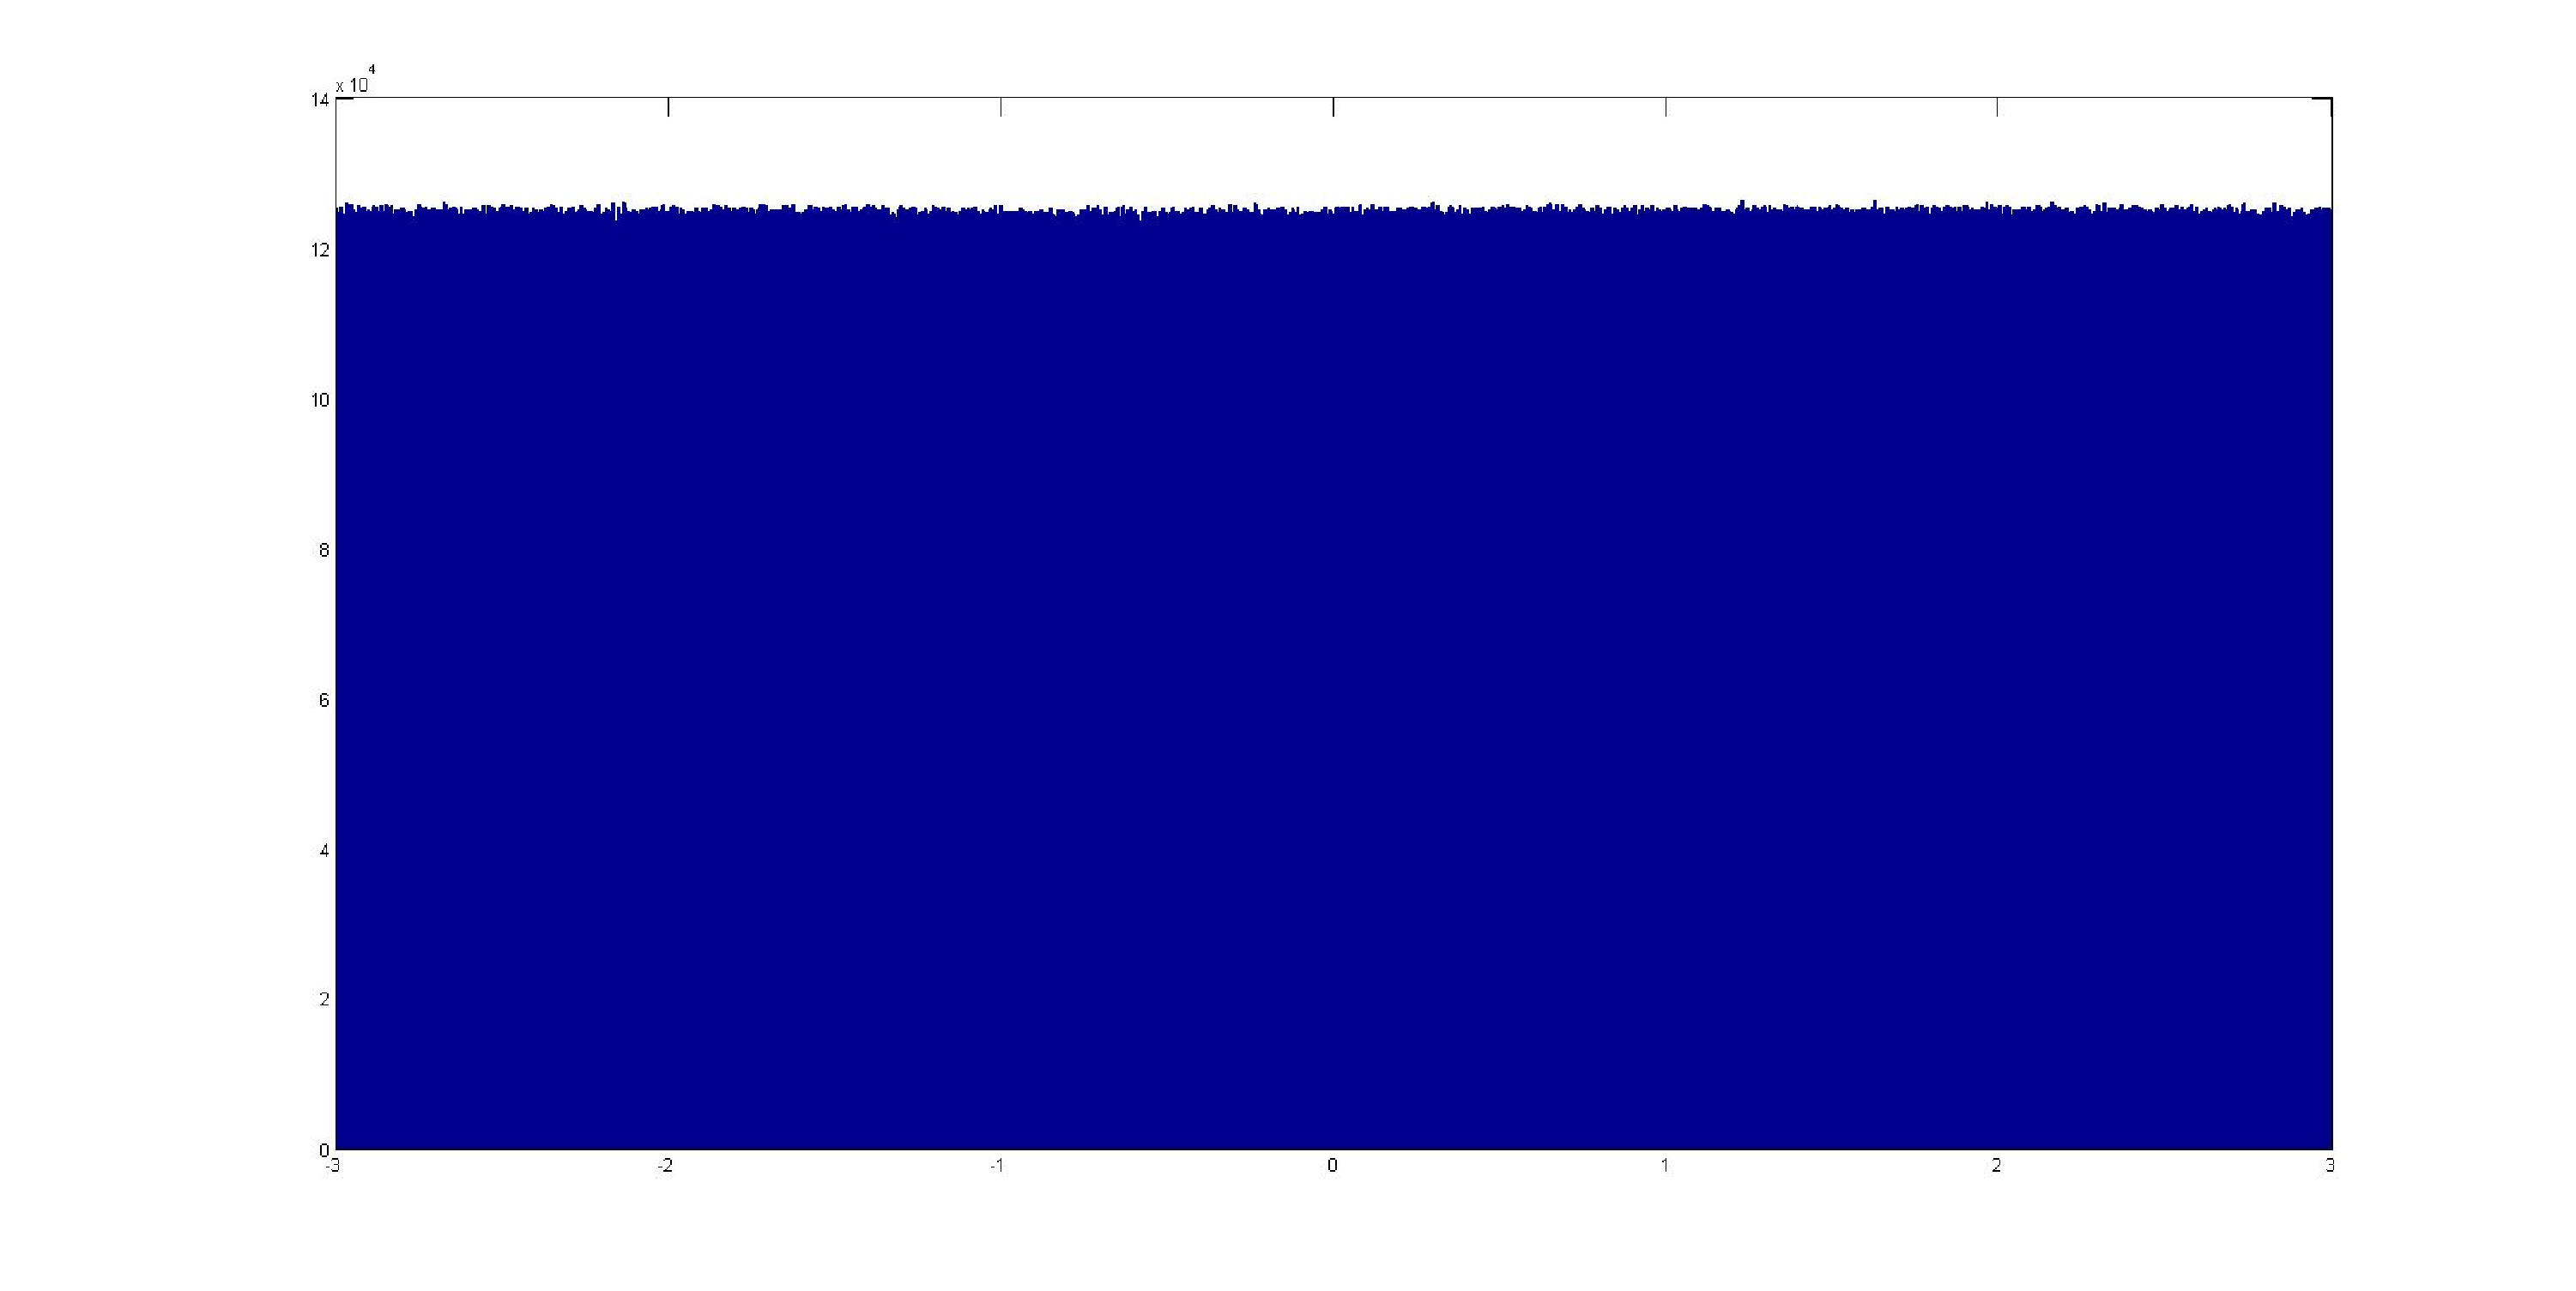
\includegraphics[width=0.45\textwidth]{rf_j_100M_1__3_3}}
\caption{Rozkład prawdopodobieństwa punktów;}
\end{figure}

\subsection{Wnioski}
W większości metod zachowanie pojedynczego punktu przekłada się na globalne zachowanie całego algorytmu. Testy pokazały cechy, które nie były oczywiste podczas prostej analizy algorytmów.

Z perspektywy algorytmu CMA-ES warto zwrócić uwagę przede wszystkim na metody zawijania i reinicjacji. W tych metodach wartości oczekiwane punktów znajdują się daleko od rodzica. Oznacza to, że w algorytmie CMA-ES macierz kowariancji może znacząco się zniekształcać.

\pagebreak

\section{Metodyka testowania metod optymalizacji globalnej}
Funkcje posiadają charakterystyczne cechy, m.in. monotoniczność, liczba ekstremów, ciągłość. Metody optymalizacji globalnej również posiadają swoje charakterystyczne własności. W zależności od przypadku, wymagania stawiane algorytmowi mogą być różne: szybkości działania, przeszukanie całej przestrzeni, czy też dokładne określenie ekstremum. Połączenie tego wszystkiego powoduje, że trudno jednoznacznie określić, która metoda optymalizacji jest najlepsza. Warto jednak posiadać wiedzę w których przypadkach metoda przynosi lepsze rezultaty.

Zapewne zgodziliby się z tym stwierdzeniem twórcy konkursów takich jak CEC, czy BBOB. Tworzą oni szereg funkcji benchmarkowych, które mają na celu empirycznie pokazać silne i słabe strony algorytmów w konkretnych sytuacjach.

\subsection{Funkcje benchmarkowe}
Funkcje benchmarkowe, to złożone funkcje. Skomplikowanie polega między innymi na wielu ekstremach funkcji lub specyficznym umieszczeniu minimum globalnego. Dzięki nim można porównać algorytmy.

\subsection{Techniki porównywania wyników}
Wybranie funkcji benchmarkowych nie wystarczy, aby stwierdzić który z algorytmów ewolucyjnych jest lepszy. Są to algorytmy niedeterministyczne - poszukiwanie rozwiązania za każdym razem będzie wyglądało inaczej nawet przy takich samych parametrach. Oznacz to, że dla wiarygodności wyników należy testy uruchamiać wielokrotnie. Posiadając takie wyniki należy posłużyć się wybraną metodą, aby porównać skuteczność algorytmów. W tej pracy do porównywania został wybrany test Wilcoxona, ponieważ można go użyć do porównywania par obserwacji oraz ten test pokazuje różnice cech.

\subsubsection*{Test Wilcoxona}
Test Wilcoxona jest testem nieparametrycznym - nie jest potrzebna wiedza na temat rozkładu populacji \cite{wilcox}. Ten test sprawdza, czy istnieje statycznie istotna różnica między dwoma zbiorami, które były losowane z pewnym rozkładem prawdopodobieństwa. Hipoteza dotyczy median wygenerowanych zbiorów. Hipoteza zerowa $H_0$ brzmi "Różnica median zbiorów wynosi 0". Na podstawie sprawdzenia hipotezy możemy wywnioskować, czy 2 rozkłady prawdopodobieństwa generują dane istotnie różne. Do przedstawienia wyników wielu testów Wilcoxona wykorzystuje się tabele.

\pagebreak

\section{Weryfikacja wpływu technik uwzględniania ograniczeń na efektywność CMA-ES}

\subsection{Cel testów}
Zrealizowanie celu całej pracy wymaga sprawdzenia, jak można usprawnić algorytm \CMAES. Trudno byłoby to zrealizować bez przetestowania samego algorytmu.

Celem testów będzie sprawdzenie charakterystycznych zachowań macierzy kowariancji. Aby zrealizować ten cel, zostaną przeprowadzone testy, które sprawdzają rozkład prawdopodobieństwa punktów. Porównana zostanie także skuteczność algorytmu CMA-ES w zależności od sposobu uwzględniania ograniczeń.

\subsection{Metoda przeprowadzenia testów}
Do przeprowadzania testów została użyta biblioteka przygotowana przez Nikolausa Hansena, współautora algorytmu CMA-ES. Tak jak w przypadku błądzenia przypadkowego, wykorzystano implementację w języku MATLAB \cite{cmaes_code}.

Testy przeprowadzano poprzez jednokrotne uruchomienie zmodyfikowanego algorytmu CMA-ES na funkcji stałej, losowej oraz kwadratowej. Modyfikacja polegała na usunięciu warunków stopu z pętli głównej algorytmu. Wynikała ona z tego, że po kilku iteracjach algorytm się zatrzymywał. Nie modyfikowano natomiast sposobu uwzględniania ograniczeń. Algorytm był przerywany po kilkuset iteracjach na podstawie logów w konsoli. Wszystkie wygenerowane przez algorytm punkty zostały przedstawione na histogramie (podobnie jak przy błądzeniu przypadkowym).

\subsection{Wyniki testów}

\subsubsection*{Funkcja stała}
Wbrew oczekiwaniom algorytm CMA-ES uruchomiony na funkcji stałej ma tendencje do zmniejszania kroku algorytmu, więc po kilkuset iteracjach przemieszczanie się wartości oczekiwanej jest znikome. Obrazują to rysunki w tym podrozdziale. Widać na nich fragmenty, w których losowane punkty były znacząco od siebie oddalone, obszar gdzie odległości pomiędzy losowanymi punktami były małe oraz miejsce, w którym algorytm prawie się nie poruszał (czerwony kwadrat)

Przeprowadzono testy, w których algorytm posiadał ograniczenie [-3; 3] na obu wymiarach oraz test bez ograniczeń.

\begin{figure}[H]
\centering
\subfloat[z ograniczeniami]{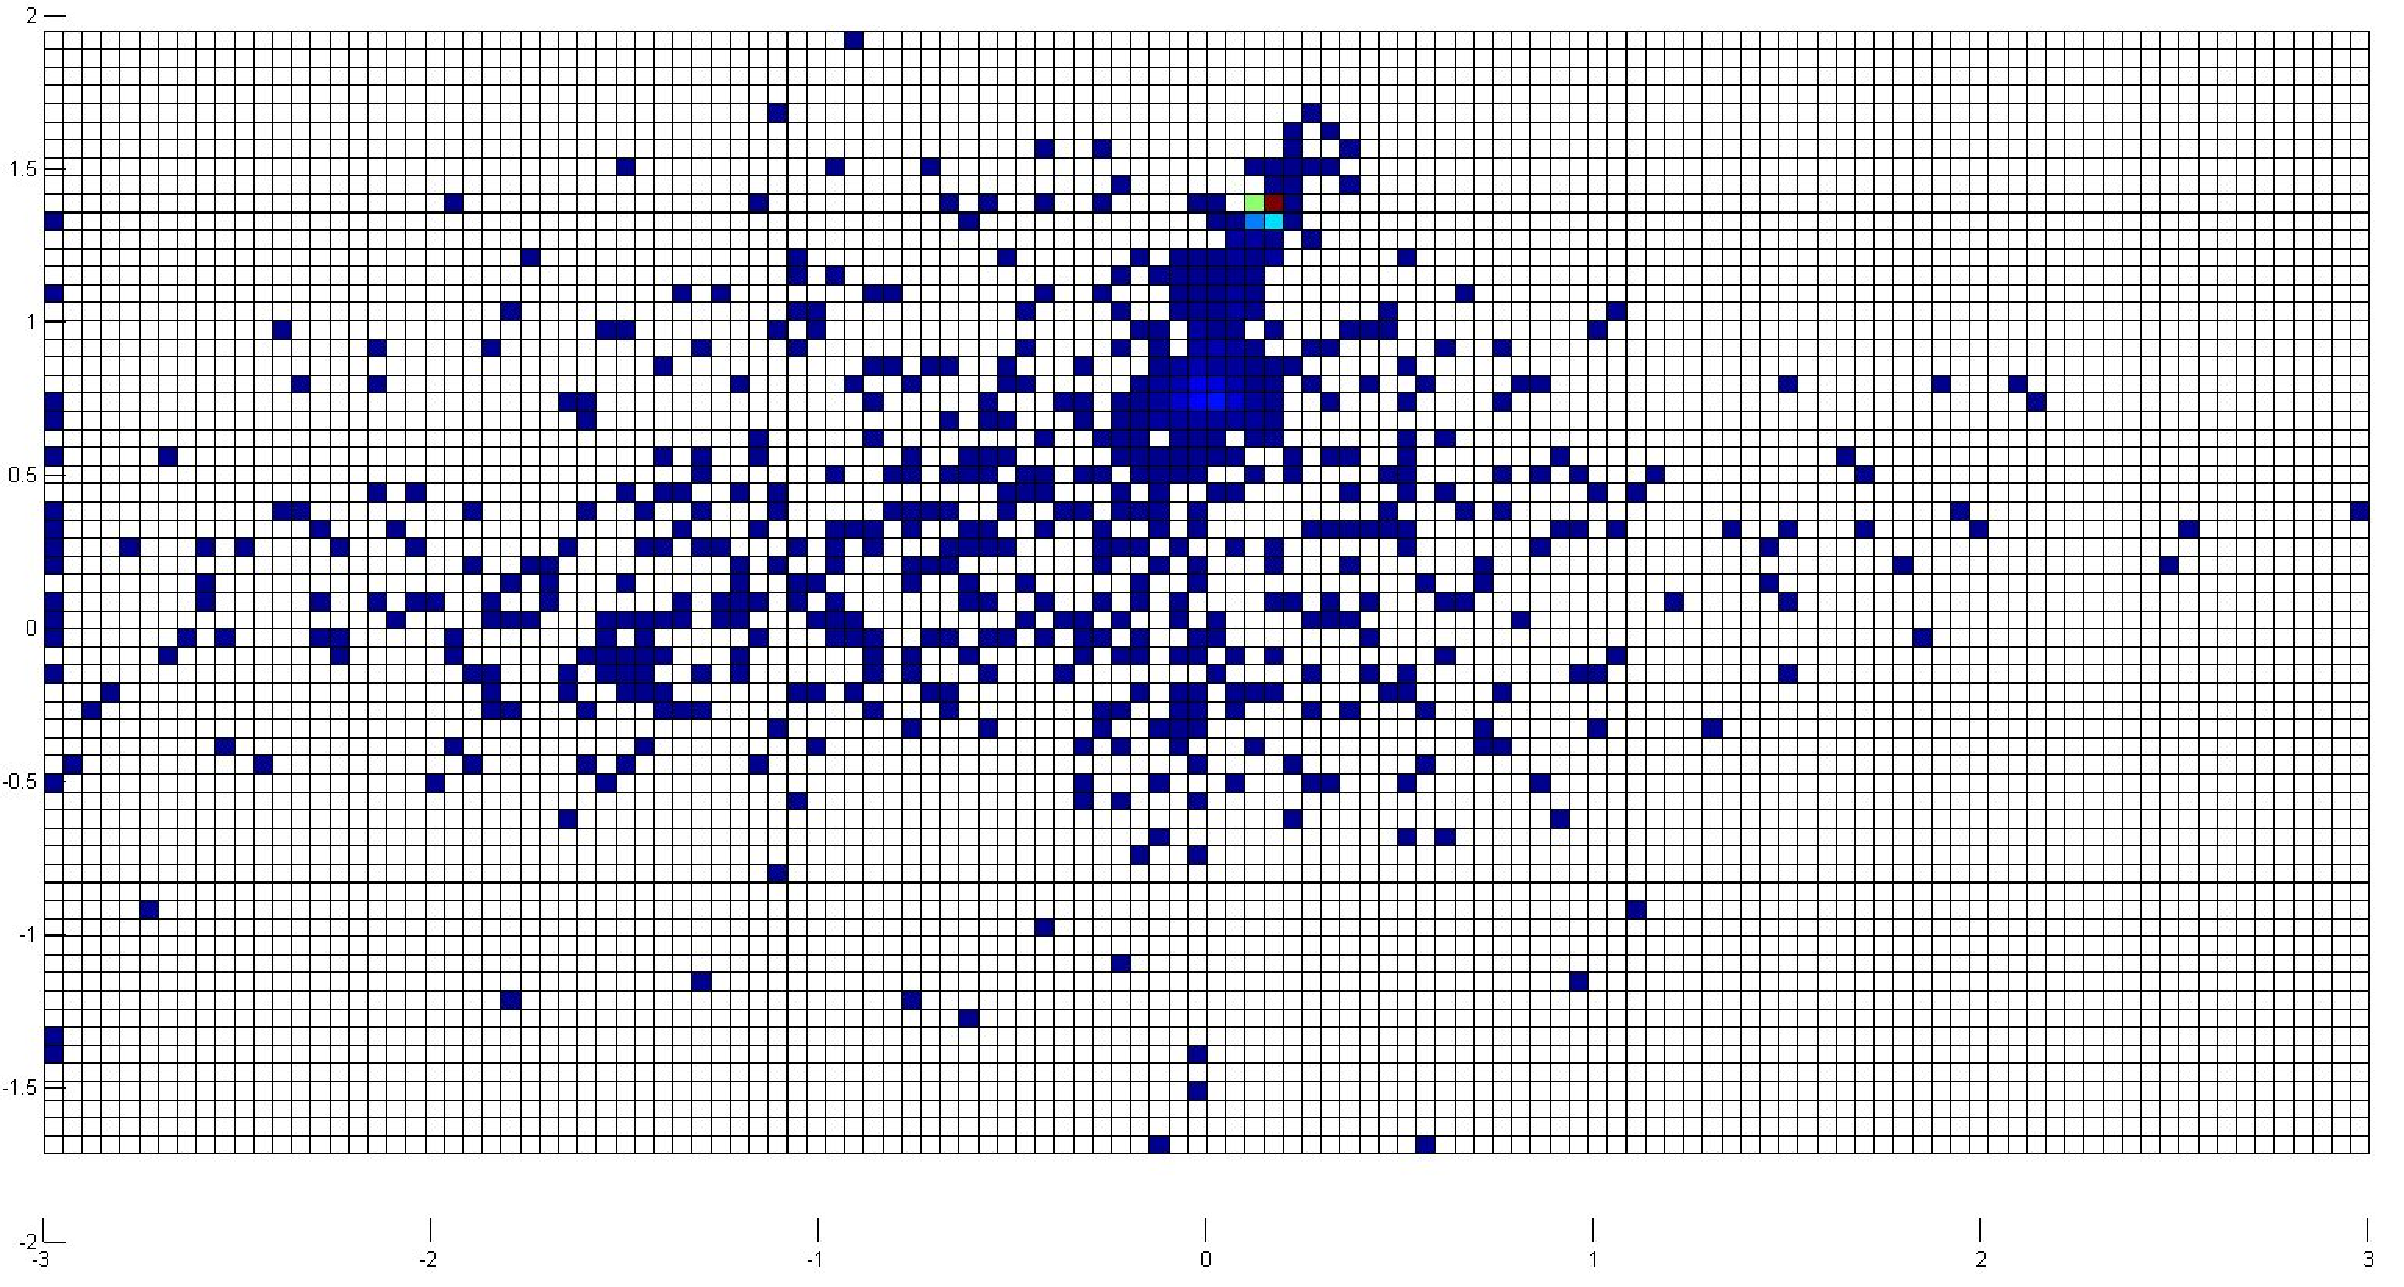
\includegraphics[width=0.45\textwidth]{cmaes-const-boundaries-dim2-start0_0}}
\quad
\subfloat[bez ograniczeń]{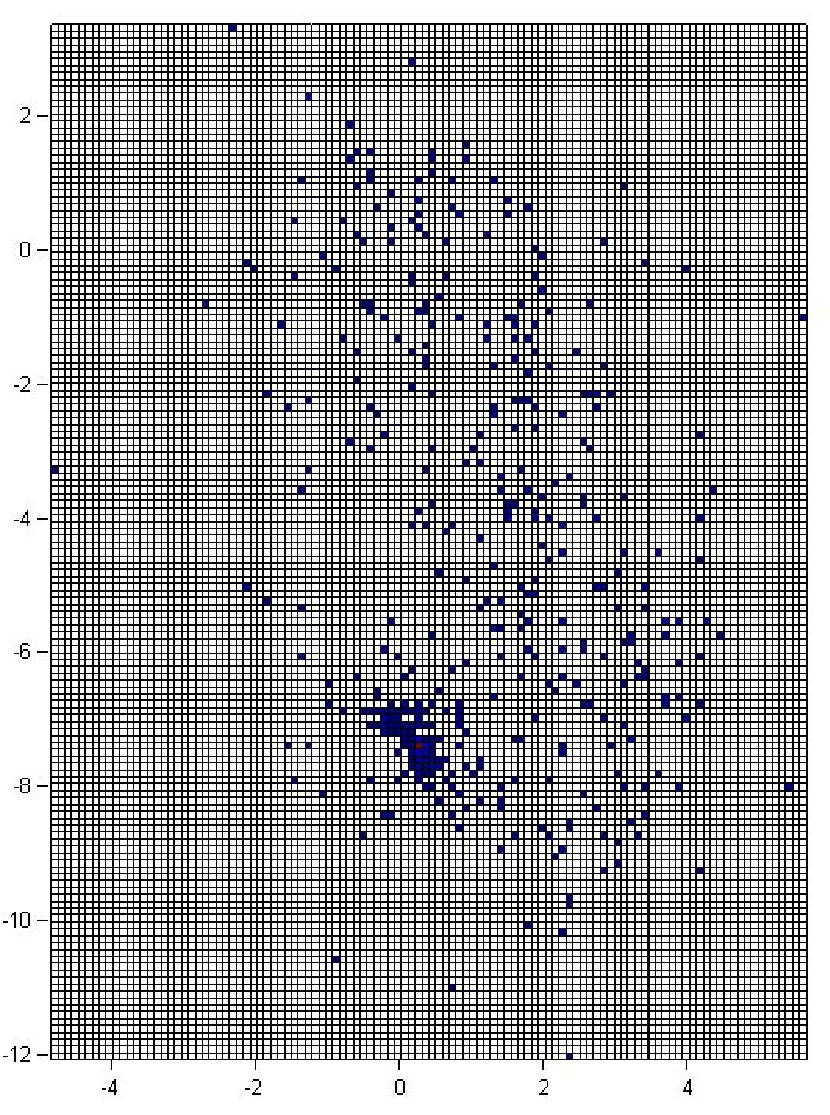
\includegraphics[width=0.45\textwidth]{cmaes-const-noboundaries-dim2-start0_0}}
\caption{Histogram punktów; algorytm CMA-ES; funkcja stała; 2 wymiary}
\end{figure}

\subsubsection*{Funkcja losowa}
Podobnie jak w przypadku obliczeń funkcji stałej, krok algorytmu CMA-ES na funkcji losowej zmniejszał się dość szybko. Poniższe wykresy, podobnie jak w przypadku testowania funkcji stałej, przedstawiają histogram wystąpień punktów w algorytmie CMA-ES z ograniczeniami oraz bez ograniczenia.

\begin{figure}[H]
\centering
\subfloat[z ograniczeniami]{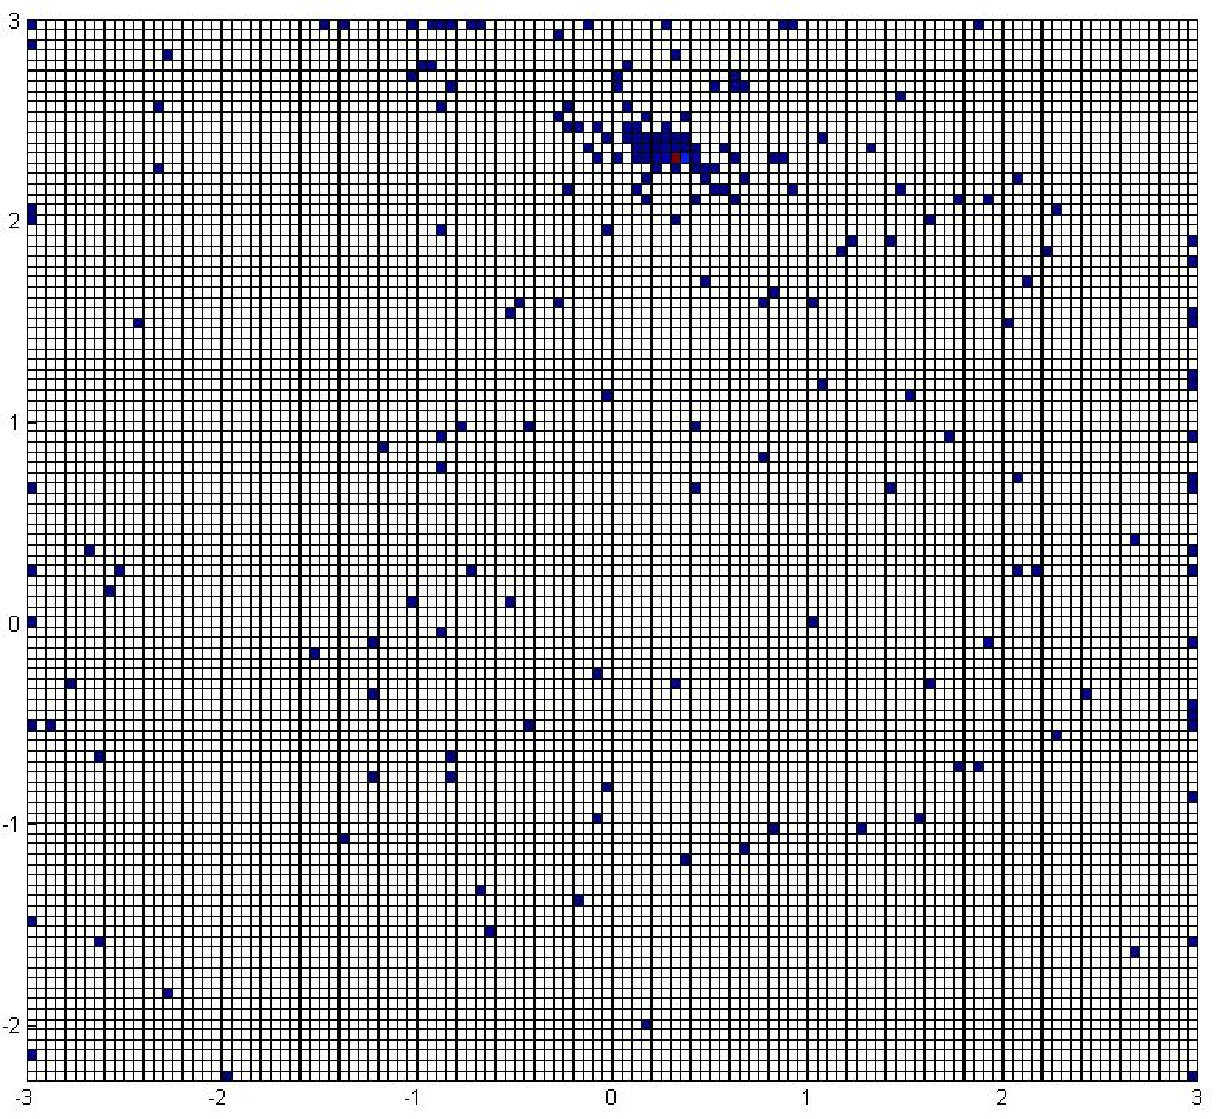
\includegraphics[width=0.45\textwidth]{cmaes-rand-boundaries-dim2-start0_0}}
\quad
\subfloat[bez ograniczeń]{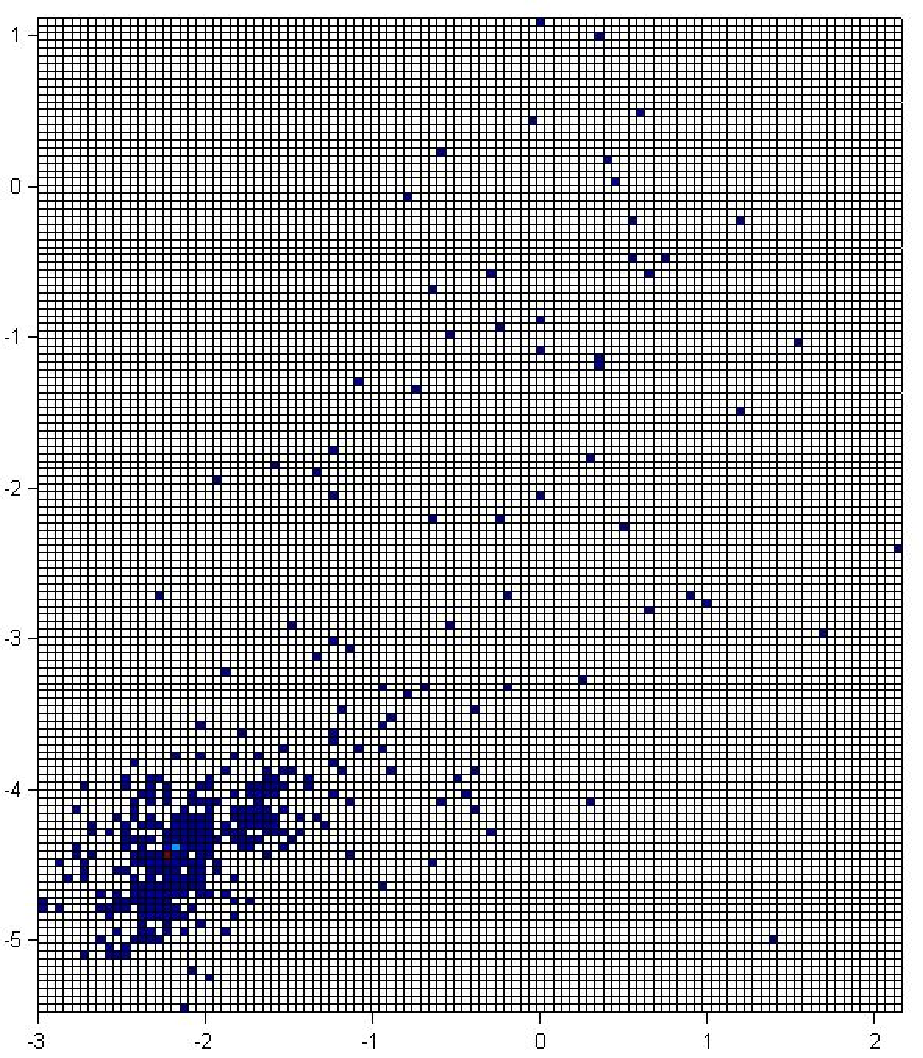
\includegraphics[width=0.45\textwidth]{cmaes-rand-noboundaries-dim2-start0_0}}
\caption{Histogram punktów; algorytm CMA-ES; funkcja losowa; 2 wymiary}
\end{figure}

\subsubsection*{Funkcja kwadratowa dwuwymiarowa}
Badano funkcję o wzorze $y=x_1^2+x_2^2$. Dla tej funkcji zdecydowano się zmienić ograniczenie. Wynosiło ono [-0,1;3] na obu wymiarach. Początkowa wartość oczekiwana wynosiła [2;2].Wykres dla tak przygotowanej symulacji znajduje się na rysunku \ref{cmaes:x2} (oś~Z została obcięta do przedziału [0;10]).

\begin{figure}[H]
\centering
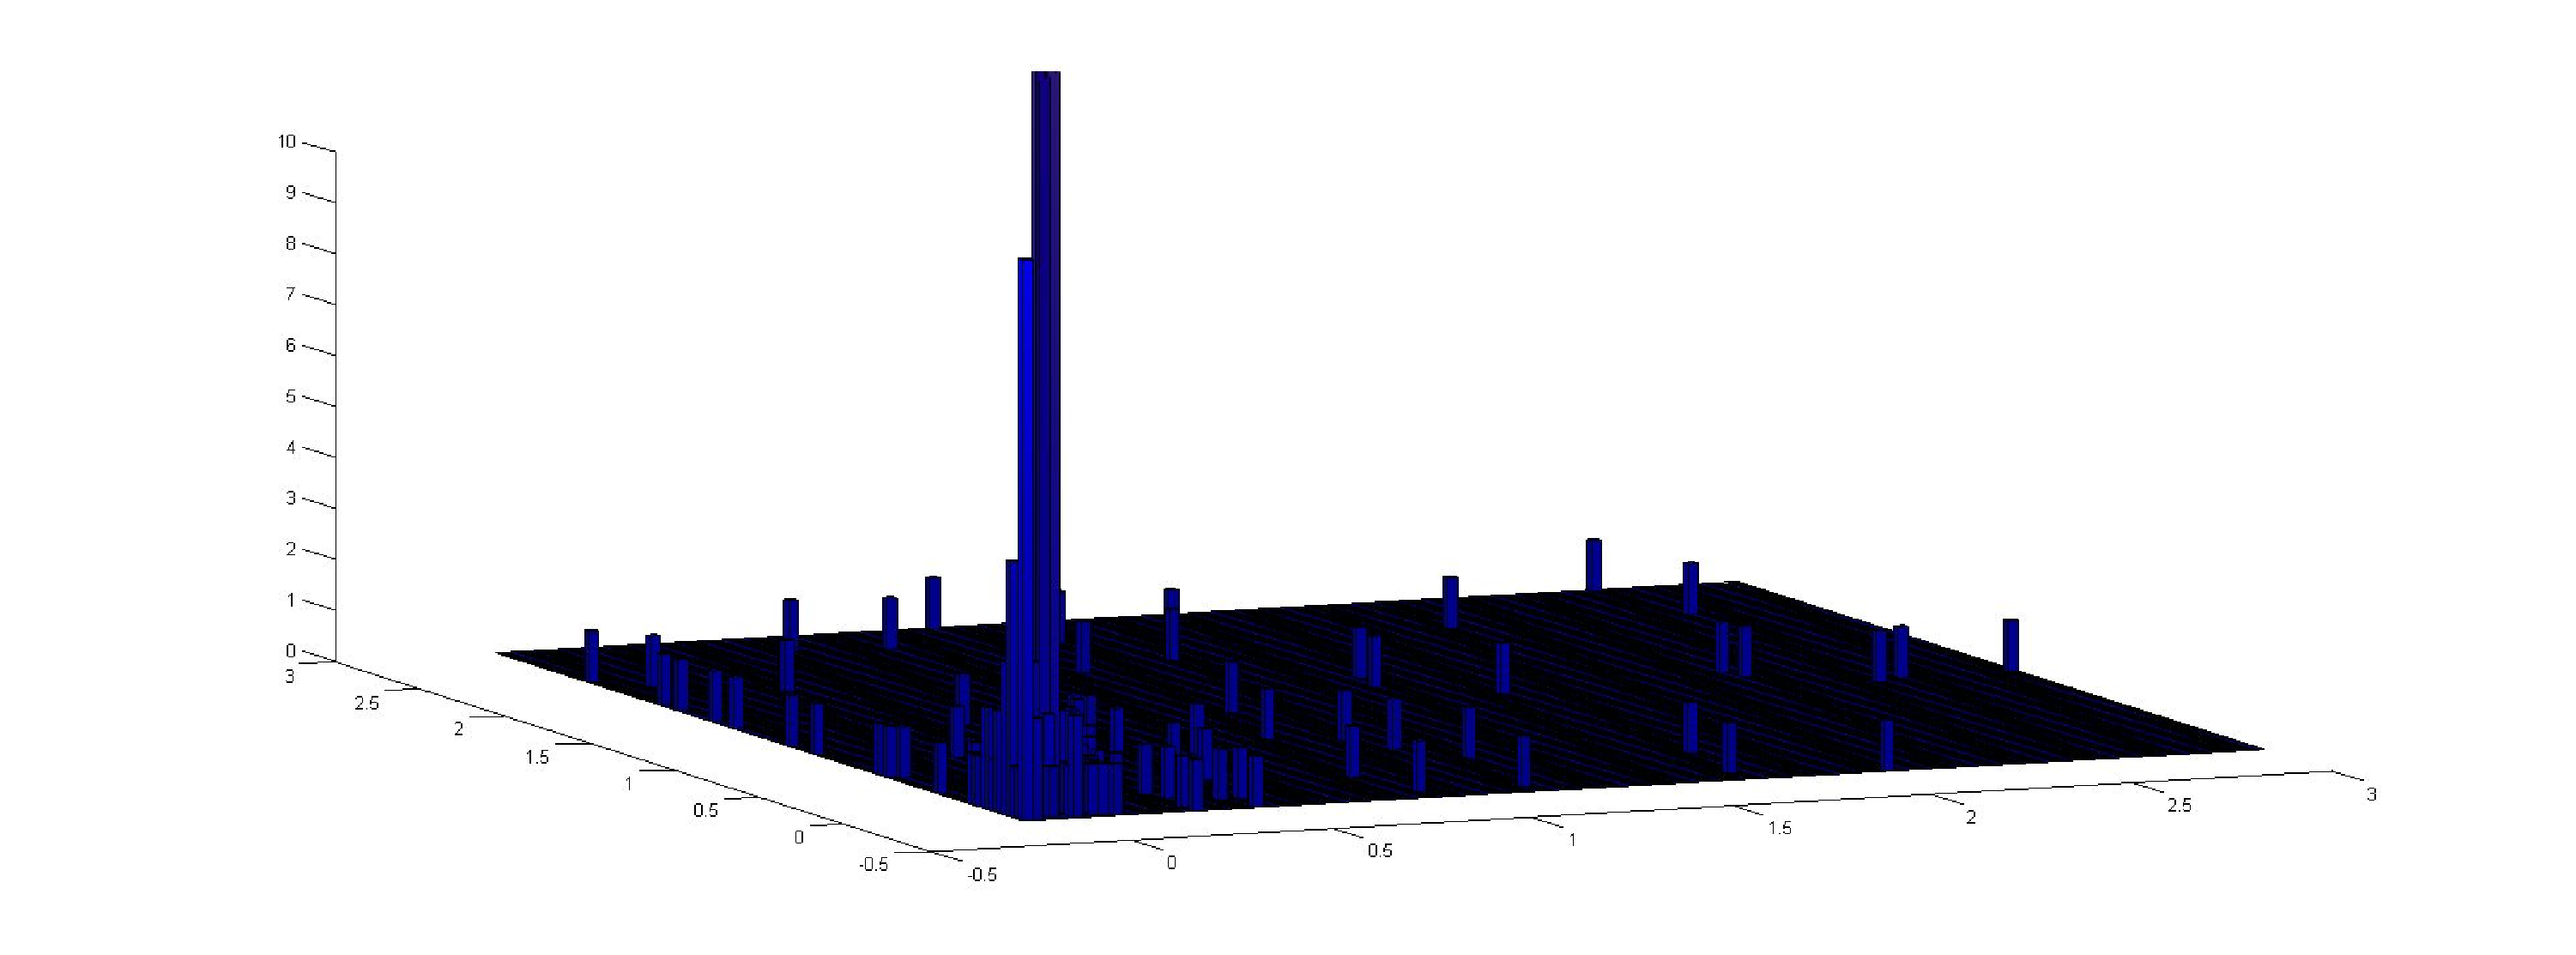
\includegraphics[width=\textwidth]{cmaes-x2dim2-boundaries-v2}
\caption{Histogram punktów; algorytm CMA-ES; funkcja losowa; 2 wymiary}
\label{cmaes:x2}
\end{figure}

\subsection{Wnioski}
Na wykresach, które przedstawiają histogramy punktów podczas symulacji algorytmu CMA-ES na funkcji losowej i stałej, nie udało się zaobserwować żadnych efektów widocznych podczas testowania błądzenia przypadkowego. Autor nie zdecydował się na generowanie wykresów innych metod transformacji rozwiązań, ponieważ nie dałoby to widocznych różnic w wykresach.

\subsection{Porównanie wariantów transformacji rozwiązań}
Celem testów było sprawdzenie, czy zmiana technik uwzględniania ograniczeń w algorytmie CMA-ES wpływa na rozwiązanie. Do tego porównania wybrano 6 wariantów transformacji rozwiązań: rzutowanie na ograniczenie (wykorzystywane w implementacji Hansena), reinicjacja, odbijanie, zawijanie, próbkowanie oraz wariant ewolucji darwinowskiej, który został opisane poniżej. Dla wszystkich wariantów uruchomiono symulacje algorytmu CMA-ES.W symulacjach wykorzystano funkcje benchmarkowe z konkursu CEC 2013, których dokładny opis znajduje się tutaj \cite{cec}. Ten zestaw został wybrany ze względu na duże zróżnicowanie funkcji oraz implementację w języku MATLAB, z której skorzystano \cite{cec_code}. Algorytm CMA-ES (dla każdego wariantu uwzględniania ograniczeń) uruchomiono po 25 razy dla każdej funkcji benchmarkowej (funkcje z 30 wymiarami). Algorytm CMA-ES dla każdej symulacji zwrócił najlepszy punkt, który znalazł. W ten sposób dla 28 funkcji uzyskano po 25 wartości. Wyniki zostały porównane testem Wilcoxona, aby sprawdzić, czy w istotny sposób się różnią.

\subsubsection*{Metoda klasyczna}
W tych testach nie znalazła się opisywana wcześniej metoda klasyczna. Wynika to z~faktu, że zakłada ona istnienie powiązań między punktami kolejnych iteracji. W~algorytmie CMA-ES wpływ punktów na kolejną iterację jest pośredni i nie ma tutaj klasycznych powiązań typu: rodzic-potomek.

\subsubsection*{Reinicjacja}
Nieco zmieniona została metoda reinicjaci. Zgodnie z rozdziałem \ref{reinicjacja} cały punkt jest przenoszony do pozycji początkowej, gdy którakolwiek z granic jest przekroczona. Takie podejście w algorytmie CMA-ES sprawiało, że algorytm zatrzymywał się w pozycji początkowej, ponieważ losowanie bardzo często zwracało punkt poza ograniczniami. Zdecydowano się na zmianę tej metody tak, że po przekroczeniu bariery reinicjowane są tylko te wymiary, na których granica została przekroczona. Pozostałe wymiary zostały bez zmian. Obrazuje to poniższy pseudokod:

\begin{Verbatim}[baselinestretch=1.1]
	dla każdej współrzędnej i
		jeżeli (lb(i) > x(i)) lub (ub(i) < x(i))
			x(i) = x0(i)
\end{Verbatim}

\subsubsection*{Ewolucja darwinowska}
Do opisania pozostła wspomniana wcześniej ewolucja darwinowska. W tym wariancie punkt nie jest transformowany wewnątrz ograniczenia. Wartość funkcji celu obliczamy w następujący sposób: kopiujemy punkt, przekształcamy symetrycznie względem tych ograniczeń, które zostały przekroczone, a na koniec obliczamy wartość funkcji dla tego punktu.

\begin{Verbatim}[baselinestretch=1.1]
	y = x
	dla każdej współrzędnej i
		jeżeli lb(i) > y(i)
			y(i) = y(i) + 2 * (lb(i) - y(i))
		jeżeli ub(i) < y(i)
			y(i) = y(i) - 2 * (y(i) - ub(i))
\end{Verbatim}

\subsubsection *{Wyniki}
Wyniki zostały przedstawione w tabeli. Do wariantu podstawowego (rzutowanie) przyrównano wyniki testu Wilcoxona pozostałych 5 wariantów. Kolumny są etykietowane numerami funkcji, natomiast wierze wariantami uwzględniania ograniczeń. Oznaczenia symboli na przecięciach:
\begin{itemize}[noitemsep]
\item + oznacza, że wariant podstawowy okazał się lepszy,
\item - oznacza, że wariant podstawowy okazał się gorszy,
\item . oznacze, że wyniki obu wariantów różnią się nieznacznie.
\end{itemize}

\begin{tabular}{|c|c|c|c|c|c|c|c|c|c|c|c|c|c|c|} \hline
Numer funkcji & 1 & 2 & 3 & 4 & 5 & 6 & 7 & 8 & 9 & 10 & 11 & 12 & 13 & 14 \\ \hline
Reinicjacja & + & . & . & . & . & . & . & . & - & . & . & . & . & - \\ \hline
Odbijanie & . & . & . & . & . & . & . & . & - & . & . & . & . & .  \\ \hline
Zawijanie  & . & . & . & . & + & . & . & . & - & . & . & . & . & - \\ \hline
Próbkowanie  & . & . & . & . & . & . & . & . & - & . & . & . & - & - \\ \hline
Darwinowska  & . & . & . & + & . & . & - & . & . & . & . & - & . & +  \\ \hline \hline
Numer funkcji & 15 & 16 & 17 & 18 & 19 & 20 & 21 & 22 & 23 & 24 & 25 & 26 & 27 & 28 \\ \hline
Reinicjacja & . & . & + & . & . & . & . & - & . & . & + & . & - & . \\ \hline
Odbijanie  & . & . & . & . & . & . & . & . & - & . & . & . & . & . \\ \hline
Zawijanie  & - & . & + & . & . & . & . & - & - & . & + & . & . & . \\ \hline
Próbkowanie & - & . & + & . & . & . & . & - & - & - & . & . & - & . \\ \hline
Darwinowska & + & . & . & . & . & . & . & + & + & . & - & . & - & . \\ \hline
\end{tabular} \\ \\

Powyższe dane pokazują, że wyniki poszczególnych algorytmów nie różnią się znacząco. Należy jednak zwrócić uwagę na wyniki próbkowania. Pokazują one, że wyniki symulacji 8 funkcji zwróciły istotnie lepsze rezulataty, niż dla symulacji z rzutowaniem. Przeciwny rezultat miał miejsce tylko dla symulacji 1 funkcji. Porównanie pozostałych algorytmów do oryginalnej implementacji nie daje wyraźnych różnic.

Warto jeszcze zwrócić, że porównanie ewolucji darwinowskiej daje inne rezultaty, niż pozostałe porównania. Pozostałe porównania posiadają pewne wspólne zachowania (podobne wyniki dla funkcji 9, 14, 17, 22).


\pagebreak

\section{Podsumowanie}
Celem pracy było sprawdzenie możliwości rozwoju algorytmu CMA-ES w obszarze ograniczeń kostkowych. Cel ten został zrealizowany poprzez teoretyczne rozważania oraz przeprowadzenie testów. Na tej podstawie tych badań wyciągnięto wnioski.

\subsection{Wnioski}
Pierwszym wnioskiem jest fakt, że ograniczenia kostkowe wpływają na rozkład prawdopodobieństw symulacji. Oznacz to, że połączenie pewnych funkcji i ograniczeń kostkowych da lepsze rezulataty.

Kolejnym wnioskiem jest to, że próbkowanie daje lepsze rezultaty od rzutowania w algorytmie CMA-ES. Należy jednak pamiętać, że próbkowanie jest bardziej czasochłonne ze względu na konieczność ponowne losowania punktów.

\subsection{Możliwości rozwoju}


\pagebreak

\begin{thebibliography}{9}

\bibitem{wyklady}
\emph{Wykłady z algorytmów ewolucyjnych}, Jarosław Arabas, 2004

\bibitem{wilcox}
\emph{The Wilcoxon Signed-Rank Test}, Richard Lowry, \url{http://vassarstats.net/textbook/ch12a.html}

\bibitem{magist}
\emph{Różnicowa implementacja algorytmu CMAES}, Michał Bobowski, 2015

\bibitem{probability}
\emph{An Introduction to Probability Theory and its Applications, Volume II}, William Feller, 1970

\bibitem{cmaes}
\emph{Completely Derandomized Self-Adaptation in Evolution Strategies} w \emph{Evolutionary Computation}, 9(2), pp. 159-195, Nikolaus Hansen, Andreas Ostermeier, 2001

\bibitem{cmaes_code}
\emph{CMA-ES: Evolution Strategy with Covariance Matrix Adaptation for nonlinear function minimization}, Nikolaus Hansen, \url{https://www.lri.fr/~hansen/cmaes\_inmatlab.html}

\bibitem{cmaes_tutorial}
\emph{The CMA evolution strategy: A tutorial. arXiv:1604.00772v1}, Nikolaus Hansen, 2016

\bibitem{cec}
\emph{Problem Definitions and Evaluation Criteria for the CEC 2013 Special Session on Real-Parameter Optimization}, J. J. Liang, B. Y. Qu, P. N. Suganthan, Alfredo G. Hernández-Díaz, 2013

\bibitem{cec_code}
\emph{CEC13 Test Function Suite }, Jane Jing Liang, \url{http://web.mysites.ntu.edu.sg/epnsugan/PublicSite/Shared%20Documents/CEC2013/cec13matlab.zip}

\bibitem{zast}
\emph{Algorytmy ewolucyjne i ich zastosowania} w \emph{Zeszyty naukowe}, 1/2006, pp. 81-92, Ewa Figielska, 2006

\bibitem{lcmaes}
\emph{Reducing the Space-Time Complexity of the CMA-ES}, James N. Knight, Monte Lunacek, 2007

\end{thebibliography}

\makestatement

\end{document}


